%!TEX root = ../thesis.tex
% ******************************* Thesis Appendix A ****************************

\setcounter{chapter}{-1}

\chapter[]{Supplementary figures} 

\ifpdf
\graphicspath{{Appendix/Figs/pdf/}}
\else
\graphicspath{{Appendix/Figs/svg/}}
\fi

\renewcommand{\thesection}{S.1}   
\section{Statistical aspects of the epigenetic clock}

\renewcommand\thefigure{S1.\arabic{figure}}    

\begin{figure}[htbp!] 
	\centering    
	\setcounter{figure}{0}
	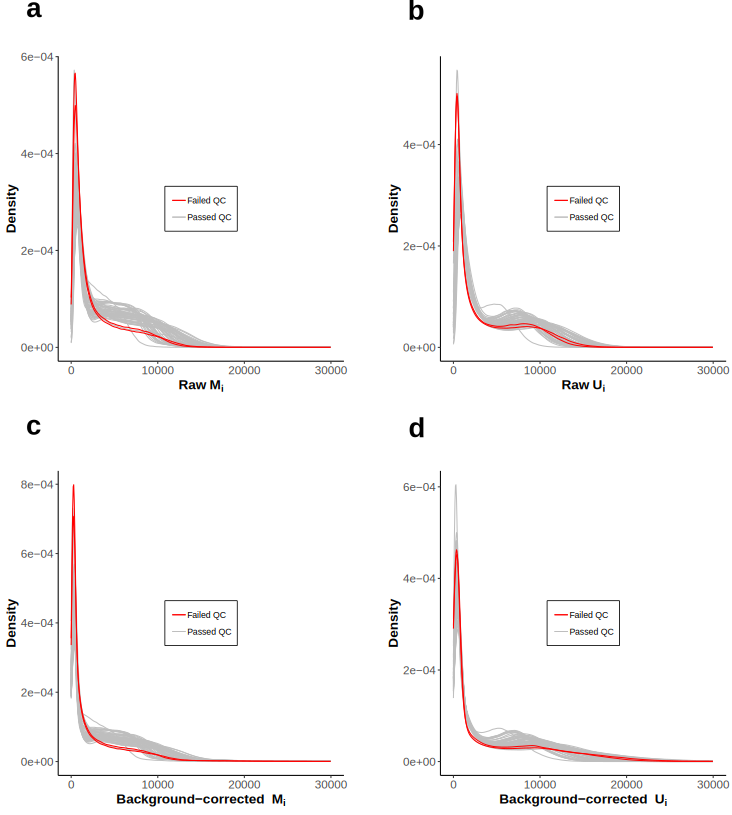
\includegraphics[width=0.62\textwidth]{SC2_Fig1}
	\caption[Effects of \textit{noob} background correction on the array fluorescence intensities.]{Effects of \textit{noob} background correction on the array flurescence intensities. Distributions of the array fluorescence intensities for the \textbf{a.} methylated signals ($M_{i}$) before background correction; \textbf{b.} unmethylated signals ($U_{i}$) before background correction; \textbf{c.} methylated signals ($M_{i}$) after background correction and \textbf{d.} unmethylated signals ($U_{i}$) after background correction. Each curve represents a DNA methylation sample from the GSE41273 batch. In grey: 51 samples that passed quality control (QC). In red: 2 samples that failed QC.}
	\label{fig:sc2_fig1}
\end{figure}

\begin{figure}[htbp!] 
	\centering    
	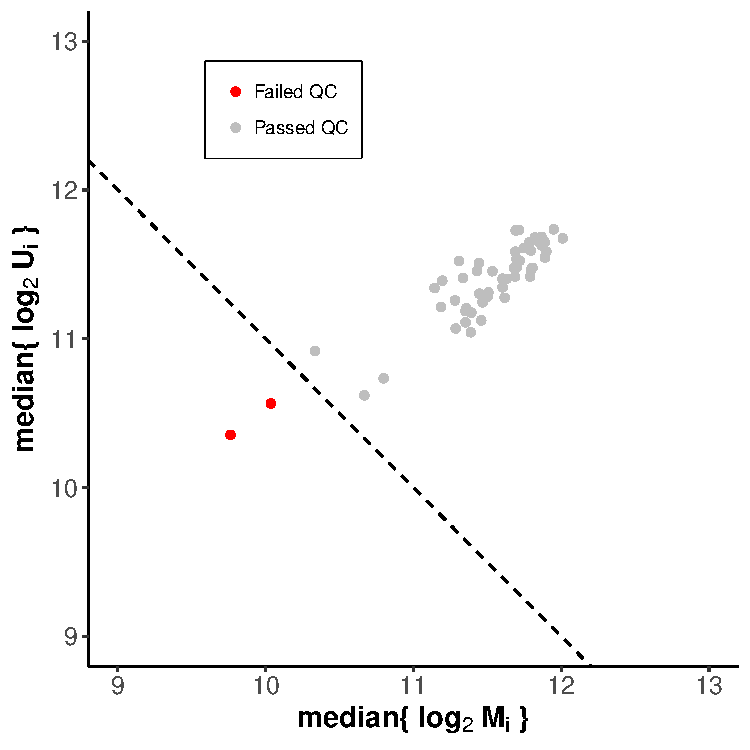
\includegraphics[width=0.5\textwidth]{SC2_Fig2}
	\caption[Quality control (QC) strategy to identify outlier samples.]{Quality control (QC) strategy to identify outlier samples, according to their global intensity values, in the GSE41273 batch. Those samples with low median intensity values (see criteria in section~\ref{s:2.1.2}) were discarded from downstream analyses (2/53, in red). Each sample is represented by one point. The dashed line represents the  intensity threshold. $M_{i}$ and $U_{i}$ represent the background-corrected methylated and unmethylated intensity measurements for the different 450K array probes in a given sample.}
	\label{fig:sc2_fig2}
\end{figure}

\begin{figure}[htbp!] 
	\centering    
	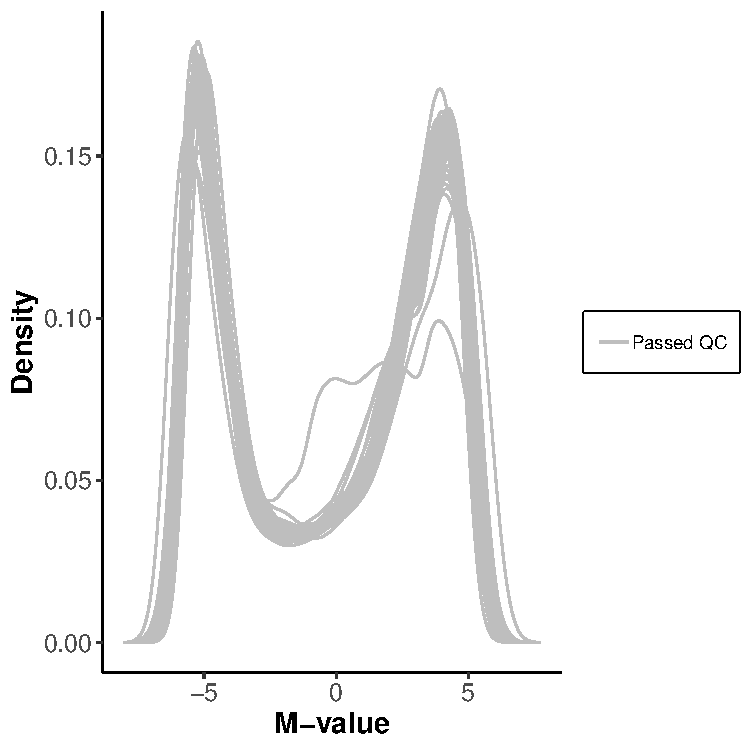
\includegraphics[width=0.5\textwidth]{SC2_Fig3}
	\caption[M-value distributions in the GSE41273 batch]{M-value distributions in the samples of the GSE41273 batch, after all the pre-processing steps have been carried out (background correction, quality control, probe filtering and BMIQ normalisation). M-values were calculated applying the logistic transformation to the $\beta$-values, as described in Du \textit{et al.} \cite{Du2010}. Each curve represents a different sample.}
	\label{fig:sc2_fig3}
\end{figure}

\begin{figure}[htbp!] 
	\centering    
	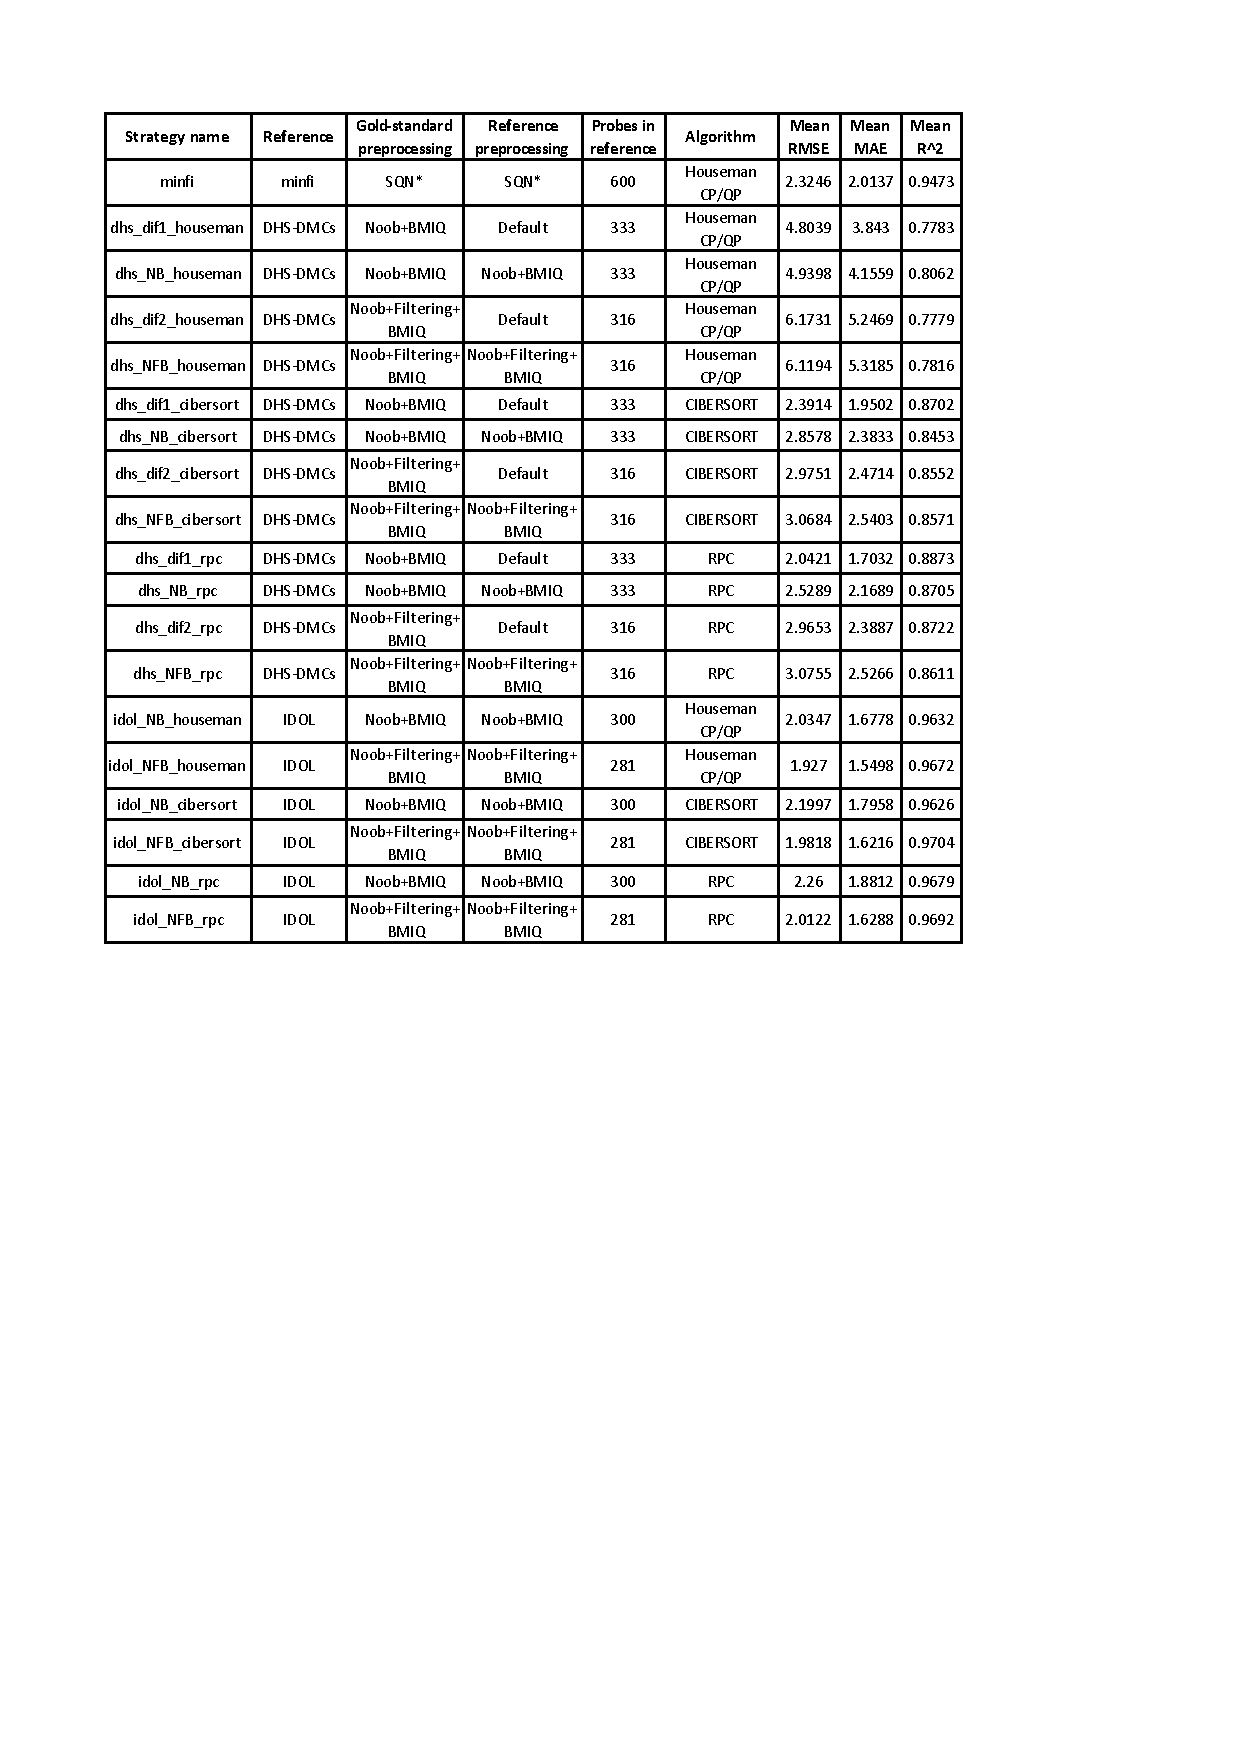
\includegraphics[width=1\textwidth]{SC2_Fig4}
	\caption[Cell-type deconvolution strategies that were benchmarked]{Table showing the different cell-type deconvolution strategies that were benchmarked. BMIQ: beta-mixture quantile normalisation. \acrshort{CP/QP}: constrained projection/quadratic programming. \acrshort{MAE}: mean absolute error. Noob: \textit{noob} background correction.  \acrshort{R$^2$}: coefficient of determination. \acrshort{RMSE}: root mean squared error. \acrshort{RPC}: robust partial correlations. \acrshort{SQN}: stratified quantile normalisation. `Default' refers to the pre-processing strategy employed in the original DHS-DMCs publication, as implemented in the \textit{EpiDISH} R package (\textit{centDHSbloodDMC.m}) \cite{Teschendorff2017a,Teschendorff2017b}. See section~\ref{s:2.1.3} in the main text for more details on what the different references refer to.}
	\label{fig:sc2_fig4}
\end{figure}

\begin{figure}[htbp!] 
	\centering    
	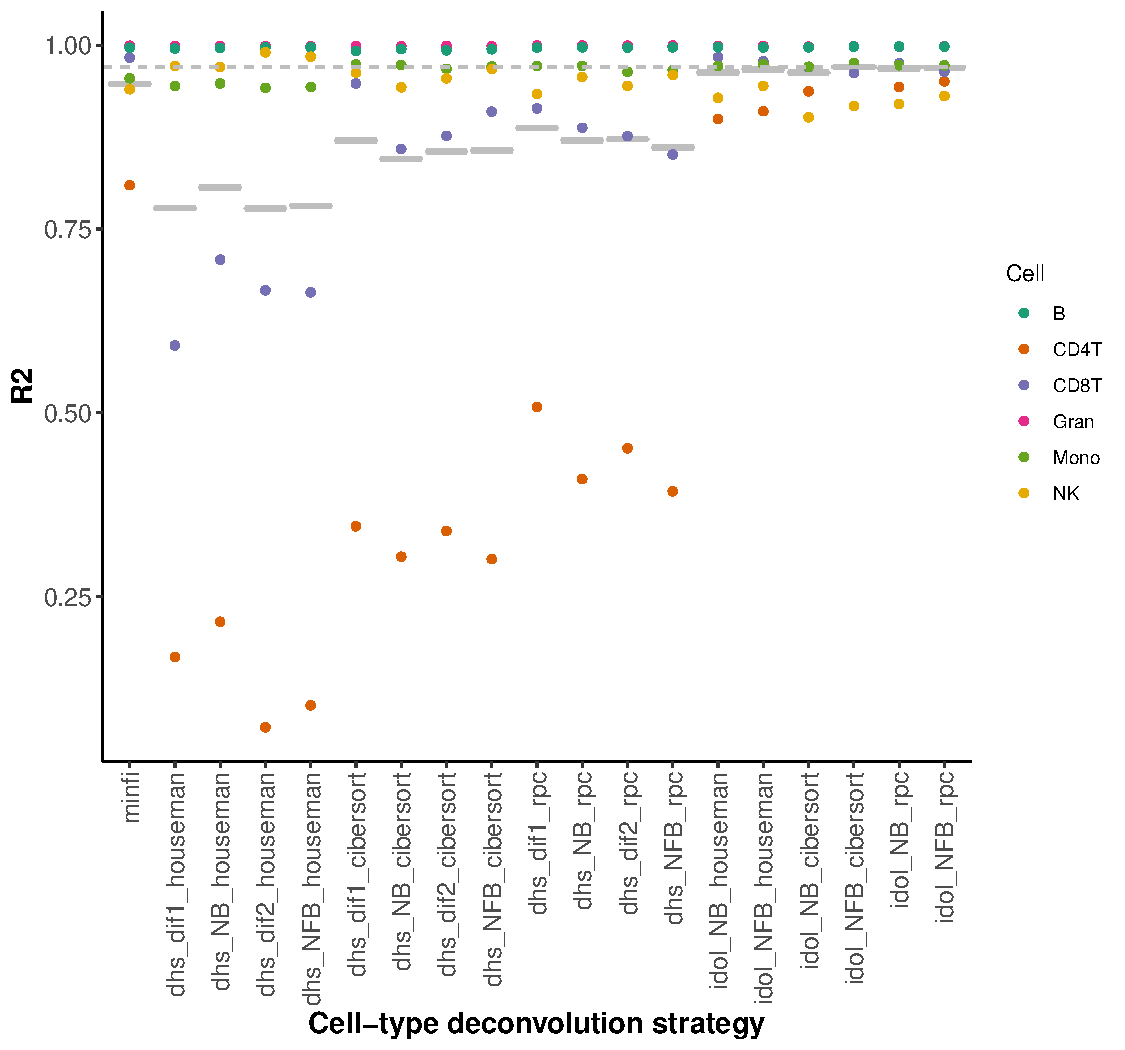
\includegraphics[width=1\textwidth]{SC2_Fig5}
	\caption[Benchmarking of the cell-type deconvolution strategies in blood: R$^2$]{Benchmarking of the cell-type deconvolution strategies in blood. The x-axis shows the different strategies that were tested (for a detailed description see Fig.~\ref{fig:sc2_fig4}). The y-axis shows the results for the coefficient of determination (R$^2$) when comparing the predictions with the real proportions of cells in a gold-standard dataset (GSE77797) \cite{Koestler2016}. The grey horizontal solid lines represent the mean for the R$^2$ across cell types and the grey dashed line the maximum of these values.}
	\label{fig:sc2_fig5}
\end{figure}

\begin{figure}[htbp!]
	\centering    
	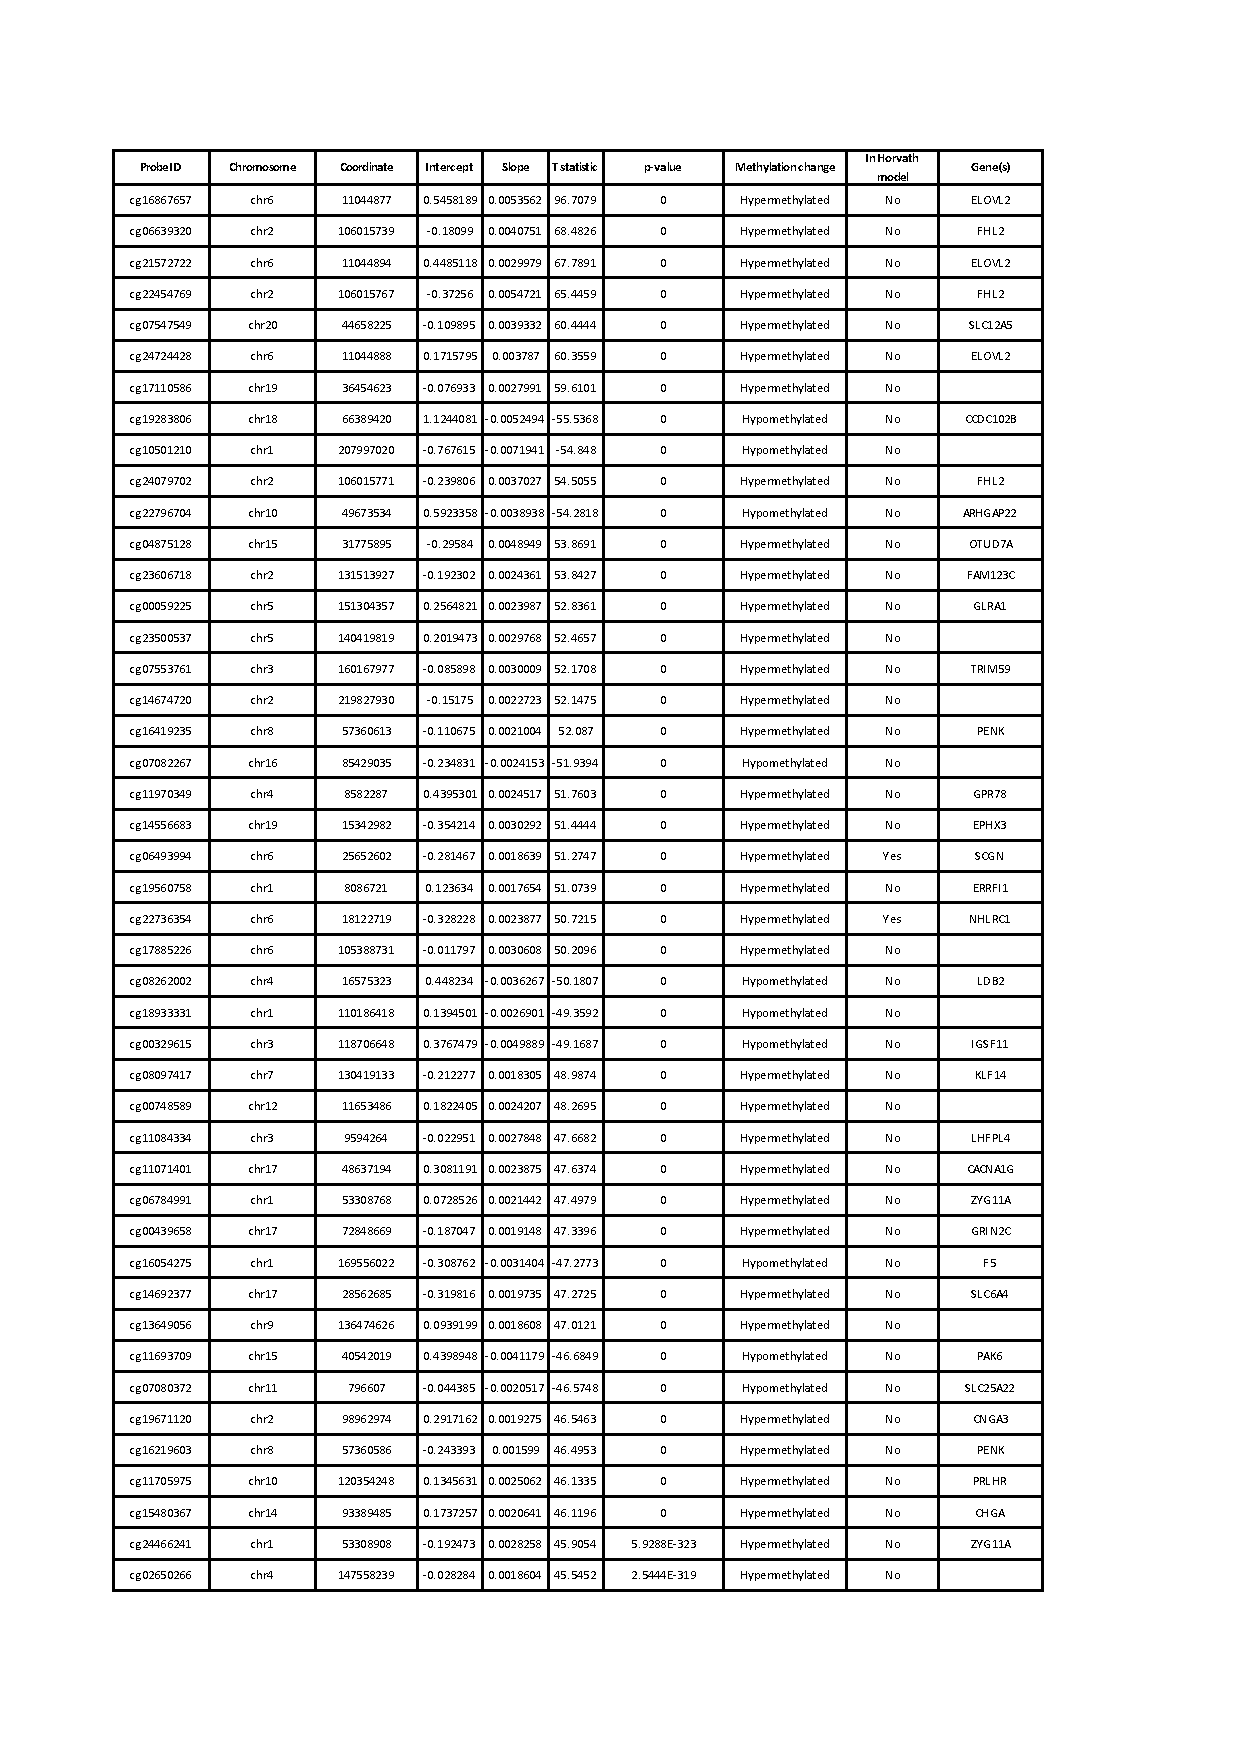
\includegraphics[width=1\textwidth]{SC2_Fig6_1}
\end{figure}
\begin{figure}[htbp!]
	\centering    
	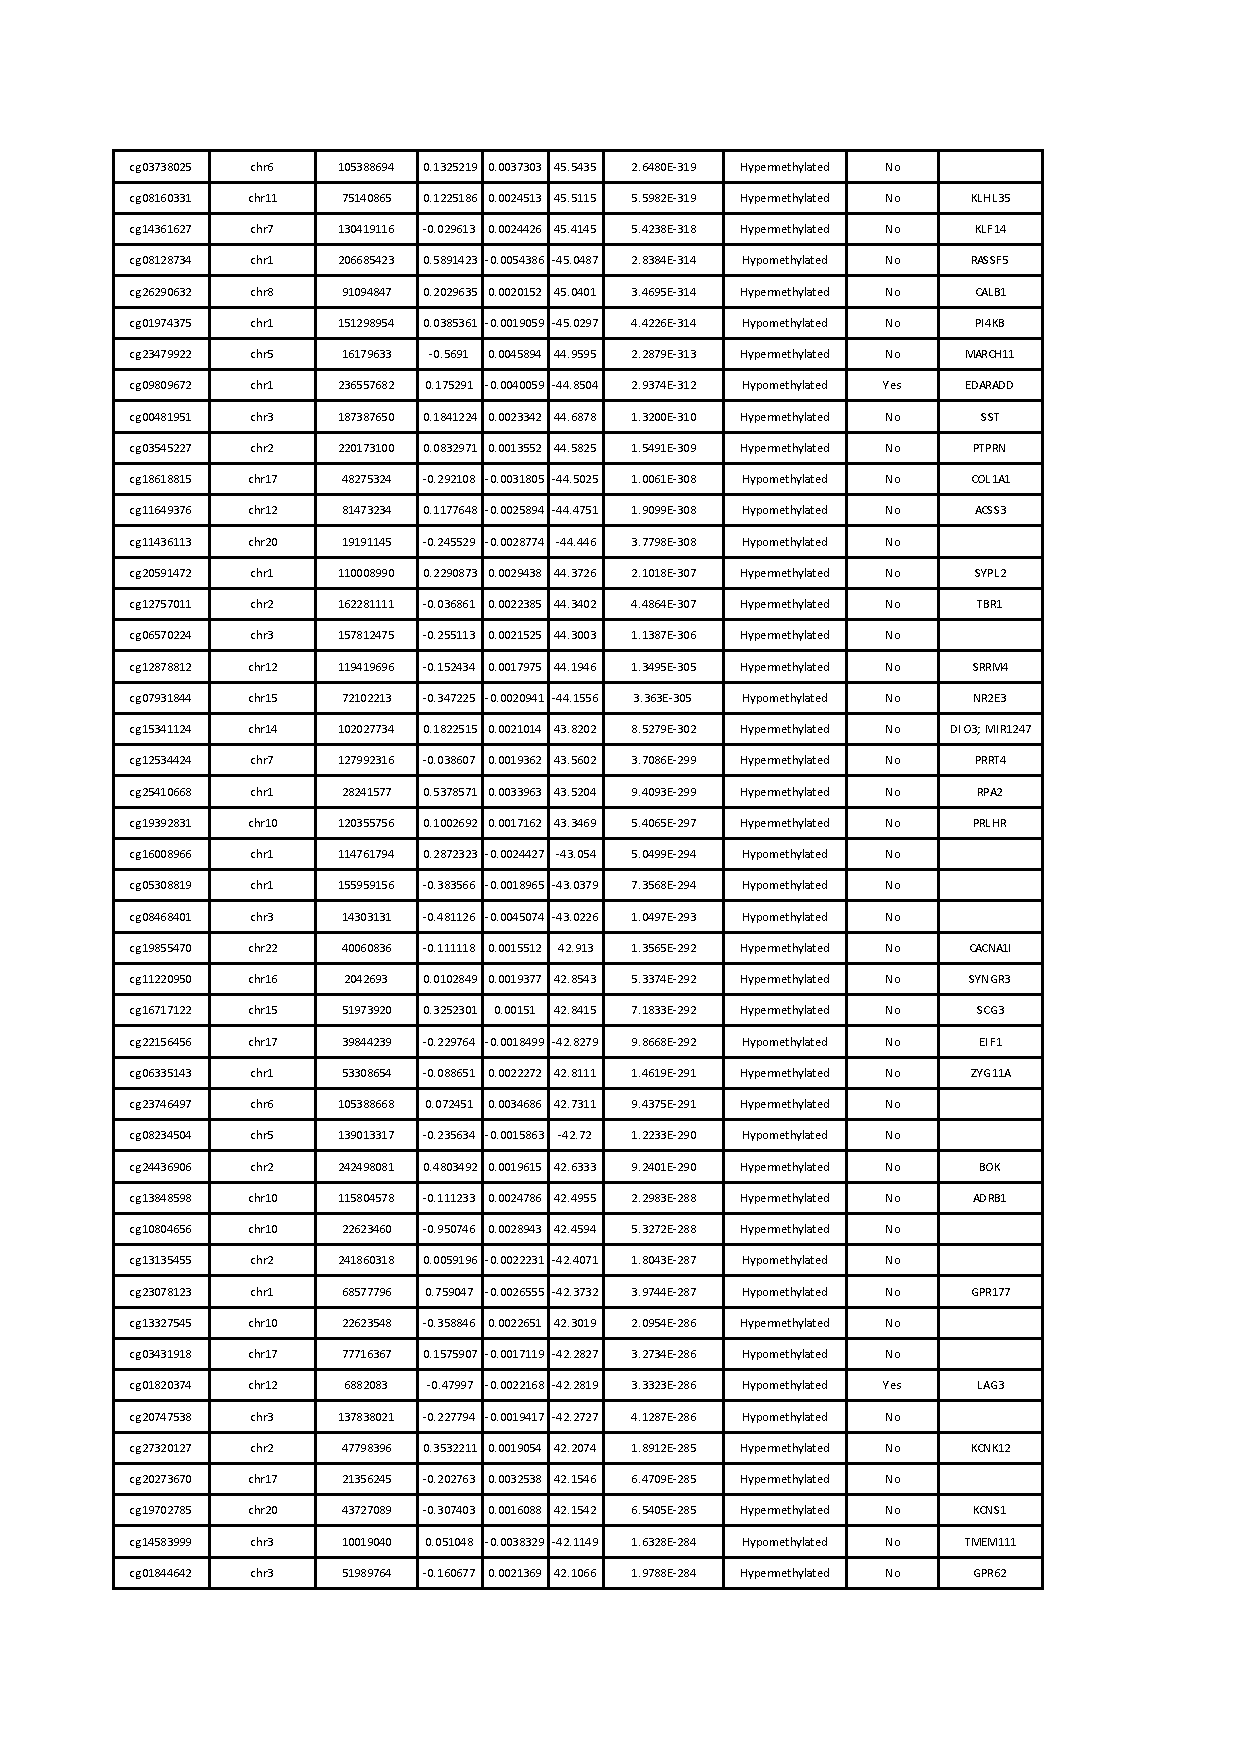
\includegraphics[width=1\textwidth]{SC2_Fig6_2}
\end{figure}
\begin{figure}[htbp!]
	\centering    
	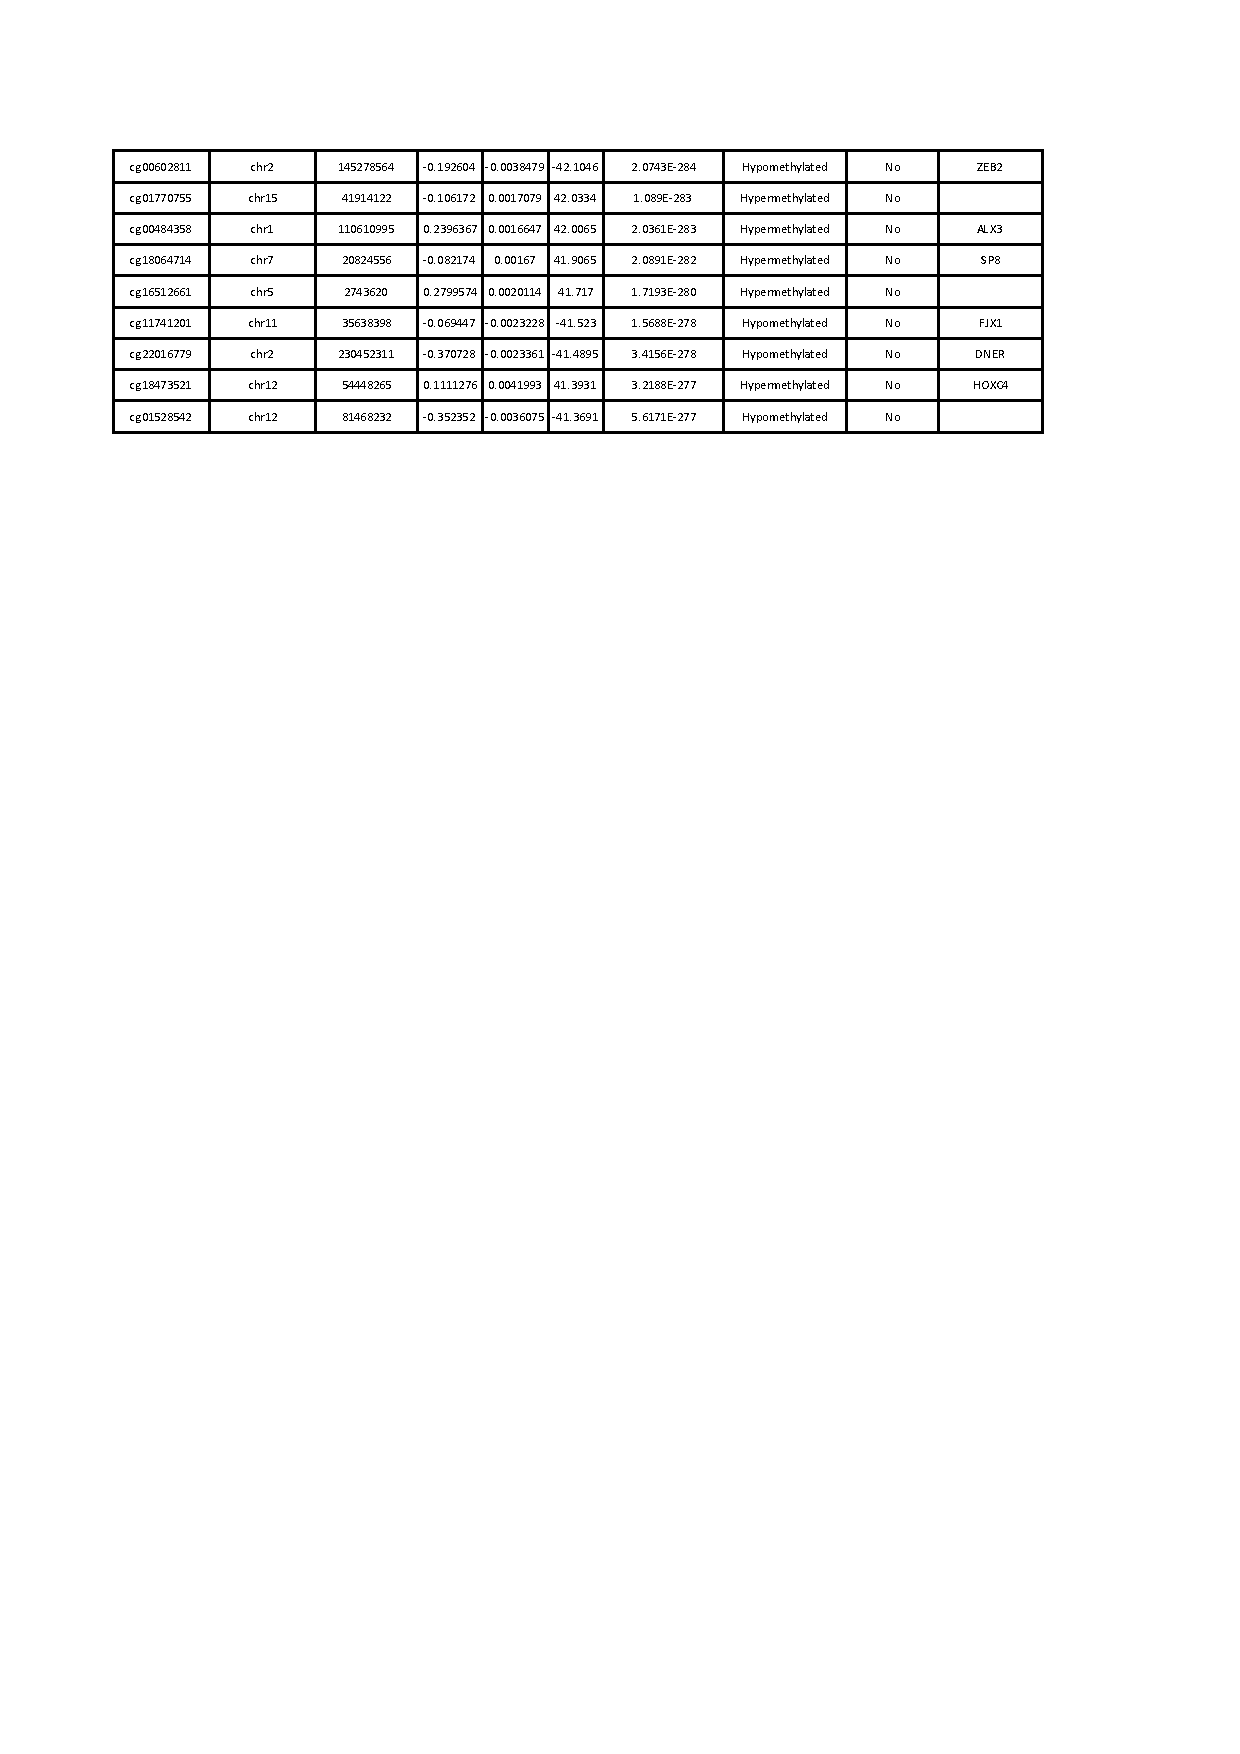
\includegraphics[width=1\textwidth]{SC2_Fig6_3}
	\caption[Table showing the top 100 aDMPs]{Table showing the characteristics of the top 100 differentially methylated positions during ageing (aDMPs) in the blood of the healthy individuals, ordered by p-value and the absolute value of the T statistic. The chromosome and coordinate refer to the \textit{hg19} human genome assembly. The reported genes are the closest genes associated with the array probe, as specified by the 450K array annotation. In this case, cell composition correction (CCC) was applied during modelling (see section~\ref{s:2.1.4}).}
	\label{fig:sc2_fig6}
\end{figure}	

\begin{figure}[htbp!] 
	\centering    
	\vspace*{3mm}
	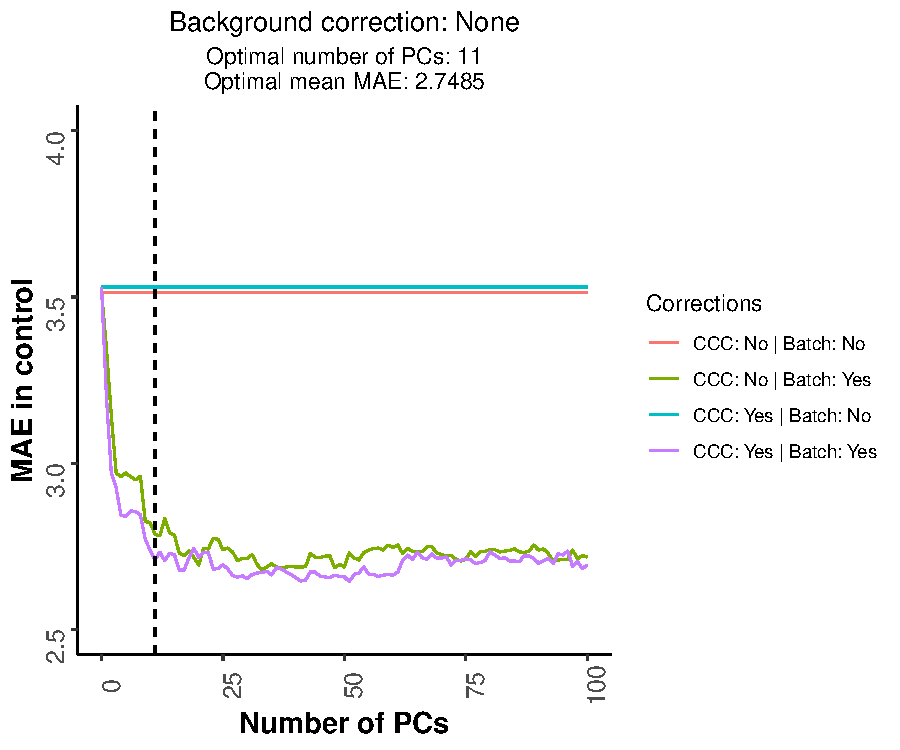
\includegraphics[width=0.8\textwidth]{SC2_Fig7}
	\caption[Impact of the absence of background correction on the predictions from the epigenetic clock]{Plot showing how the median absolute error (MAE) of the prediction in the healthy individual samples, that should tend to zero, is reduced when the PCs capturing the technical variation are included as part of the modelling strategy (see equations \ref{eq:2.16} and \ref{eq:2.17}). The dashed line represents the optimal number of PCs (11) that was finally used. The optimal mean MAE is calculated as the average MAE between the green and purple lines. In this case, no background correction was applied to the methylation data before calculating the epigenetic ages according to Horvath's epigenetic clock \cite{Horvath2013}.}
	\label{fig:sc2_fig7}
\end{figure}

\begin{figure}[htbp!] 
	\centering    
	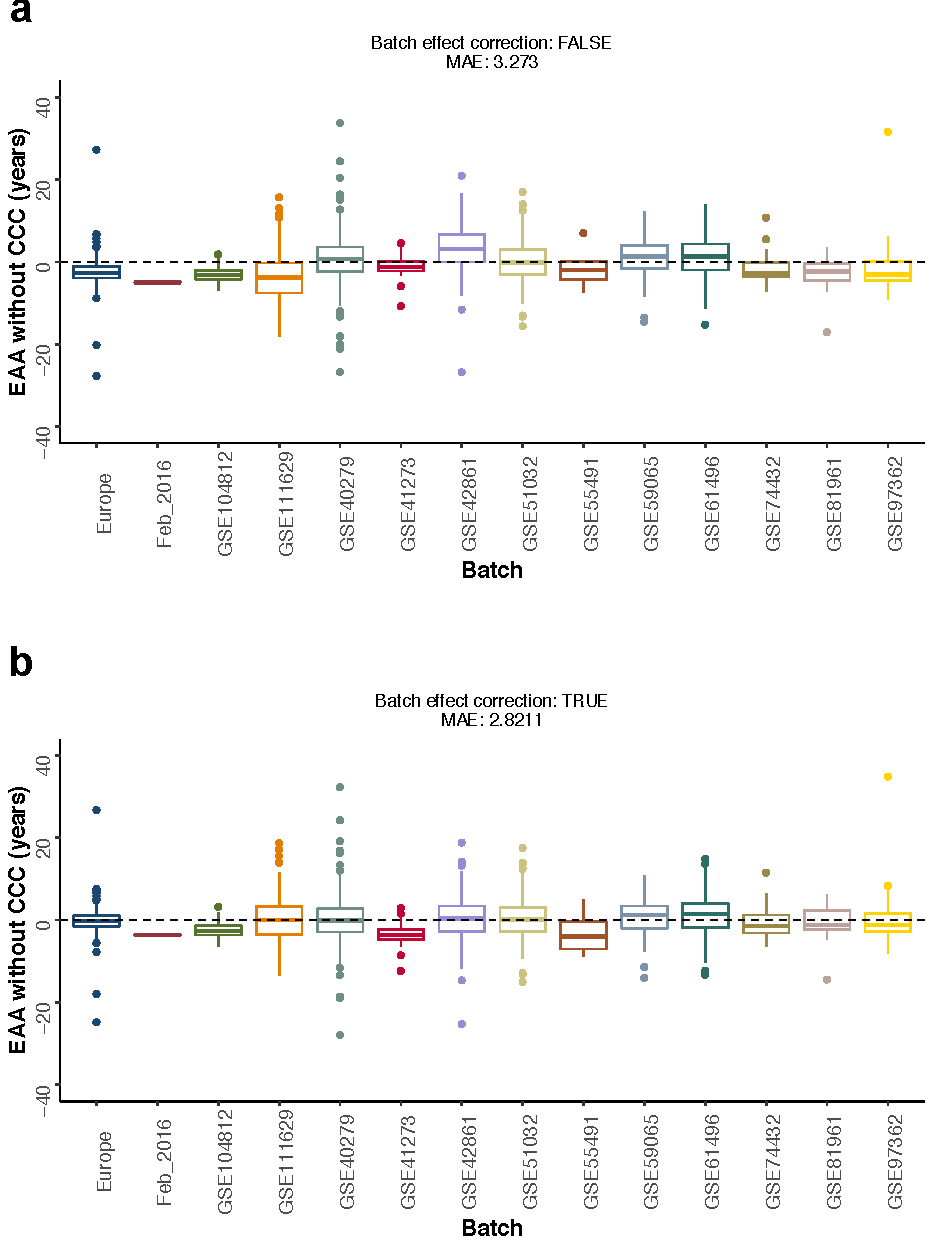
\includegraphics[width=0.9\textwidth]{SC2_Fig8}
	\caption[Correcting for batch effects: control model without cell composition correction]{Correcting for batch effects in the context of the epigenetic clock. \textbf{a.} Distribution of the epigenetic age acceleration (EAA) for the different batches of healthy individual samples, using the control model without cell composition correction (CCC) and before applying batch effect correction. The dashed black line represents $EAA = 0$, where the distributions should be centred around. \textbf{b.} As in a., but after applying batch effect correction (i.e. equivalent to equation \ref{eq:2.17}).}
	\label{fig:sc2_fig8}
\end{figure}

\begin{figure}[htbp!] 
	\centering    
	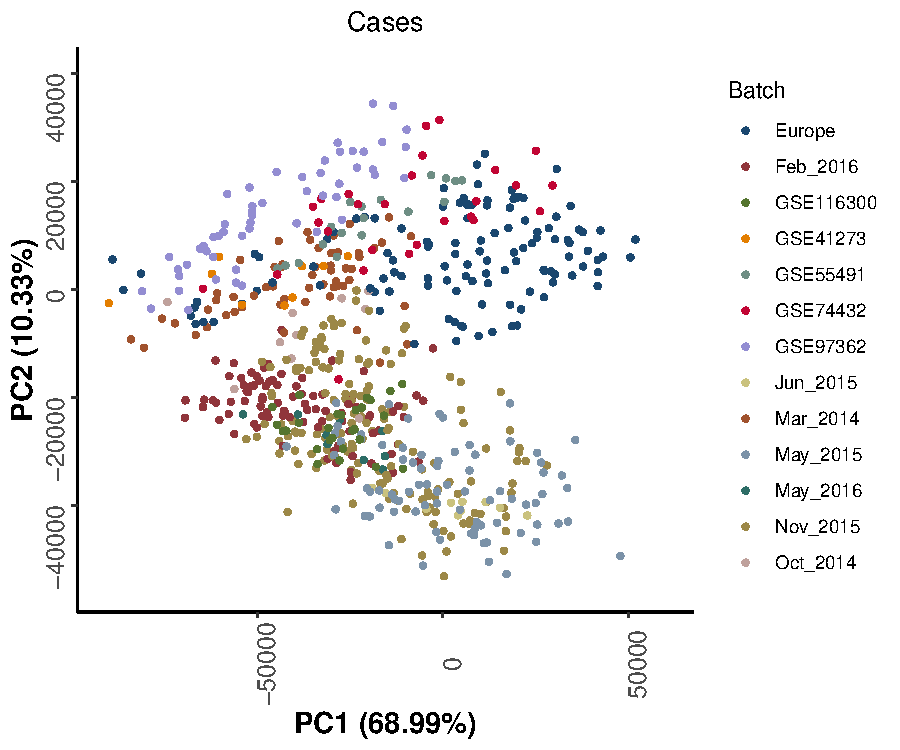
\includegraphics[width=0.7\textwidth]{SC2_Fig9}
	\caption[PCA on the array control probes captures batch effects: cases]{Scatterplot showing the values of the first two principal components (PCs) for the samples with developmental disorders (cases, see Chapter~\ref{c:3}) after performing PCA on the control probes of the 450K arrays. Each point corresponds to a different sample and the colours represent the different batches. The different batches cluster together in the PCA space, showing that the control probes indeed capture technical variation. Please note that all the PCA calculations were done using samples from both healthy individuals (full lifespan, $N=2218$) and cases from developmental disorders ($N=666$).}
	\label{fig:sc2_fig9}
\end{figure}

\begin{figure}[htbp!] 
	\vspace*{5mm}
	\centering    
	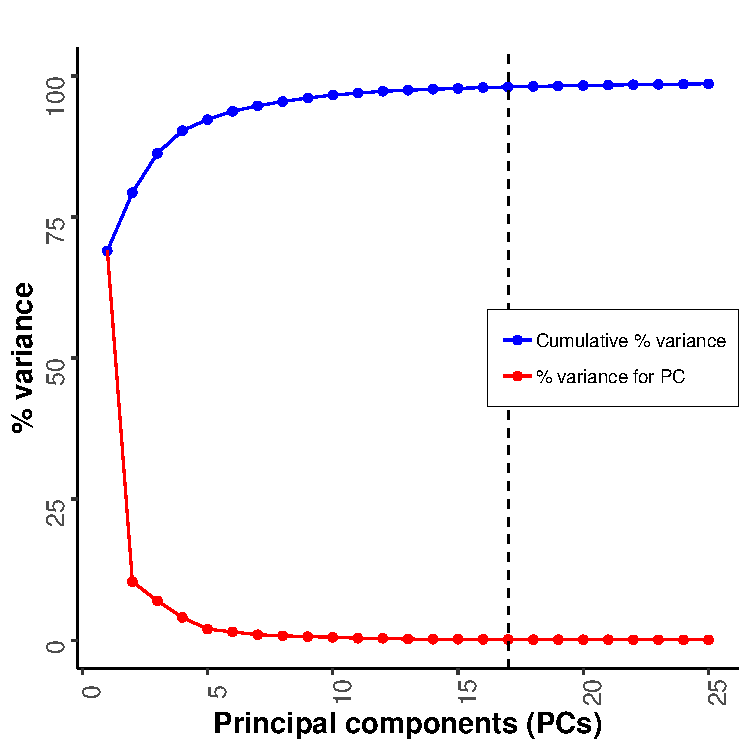
\includegraphics[width=0.5\textwidth]{SC2_Fig10}
	\caption[Variance explained by the different principal components during batch effect correction]{Plot showing the percentages of technical variance explained by the different PCs from the control probes. The dashed line represents the optimal number of PCs (17) that was finally used.}
	\label{fig:sc2_fig10}
\end{figure}

\clearpage

\renewcommand{\thesection}{S.2}   
\section{Biological aspects of the epigenetic clock}

\renewcommand\thefigure{S2.\arabic{figure}}
\renewcommand\thetable{S2.\arabic{table}}        
\vspace{10 mm}

\begin{table}[h]
	\centering
	\small
	\begin{tabular}{ p{2cm} p{1cm} p{1cm} p{1cm} p{2cm} p{6cm} }
		\toprule
		\textbf{Batch name} & \textbf{N$_{\female}$} & \textbf{N$_{\male}$} & \textbf{N} & \textbf{Median age (years)} & \textbf{Other comments} \\
		\midrule
		  Europe & 0 & 119 & 119 & 7.73 & \\
		  Feb\_2016 & 20 & 20 & 40 & 6 & \\
		  GSE116300 & 4 & 5 & 9 & 3 &\\
		  GSE41273 & 0 & 9 & 9 & 7.75 & \\
		  GSE74432 & 11 & 16 & 27 & 10 & \\
		  GSE97362 & 4 & 9 & 13 & 15 & Samples from the `validation cohort' were not included in the analysis, since they all seemed outliers on close examination\\
		  Jun\_2015 & 1 & 1 & 2 & 3.5015 & \\
		  Mar\_2014 & 11 & 6 & 17 & 8 & \\
		  May\_2015 & 17 & 49 & 66 & 14 & \\
		  Nov\_2015 & 35 & 30 & 65 & 6.7 & \\
		\midrule
		\textbf{Total} & 103 & 264 & 367 & 8 & - \\ 
		\bottomrule
	\end{tabular}
	\vspace*{3mm}
	\caption[Additional information for the developmental disorders dataset]{Overview of the blood DNA methylation dataset from individuals with developmental disorders. The batches `Europe', `Feb\_2016', `Jun\_2015', `Mar\_2014', `May\_2015' and `Nov\_2015' were generated in-house by our collaborators in Canada (see Chapter~\ref{c:3}). The rest of the batches were downloaded from GEO \cite{Edgar2002}. $N_{\female}$: number of samples from females. $N_{\male}$: number of samples from males. $N$: total number of samples. These numbers correspond to the samples left after applying quality control and filtering (see section~\ref{s:3.2}).}
	\label{table:s2_table1}
\end{table} 

\smallskip

\clearpage

\begin{figure}[htbp!]
	\setcounter{figure}{0}
	\centering    
	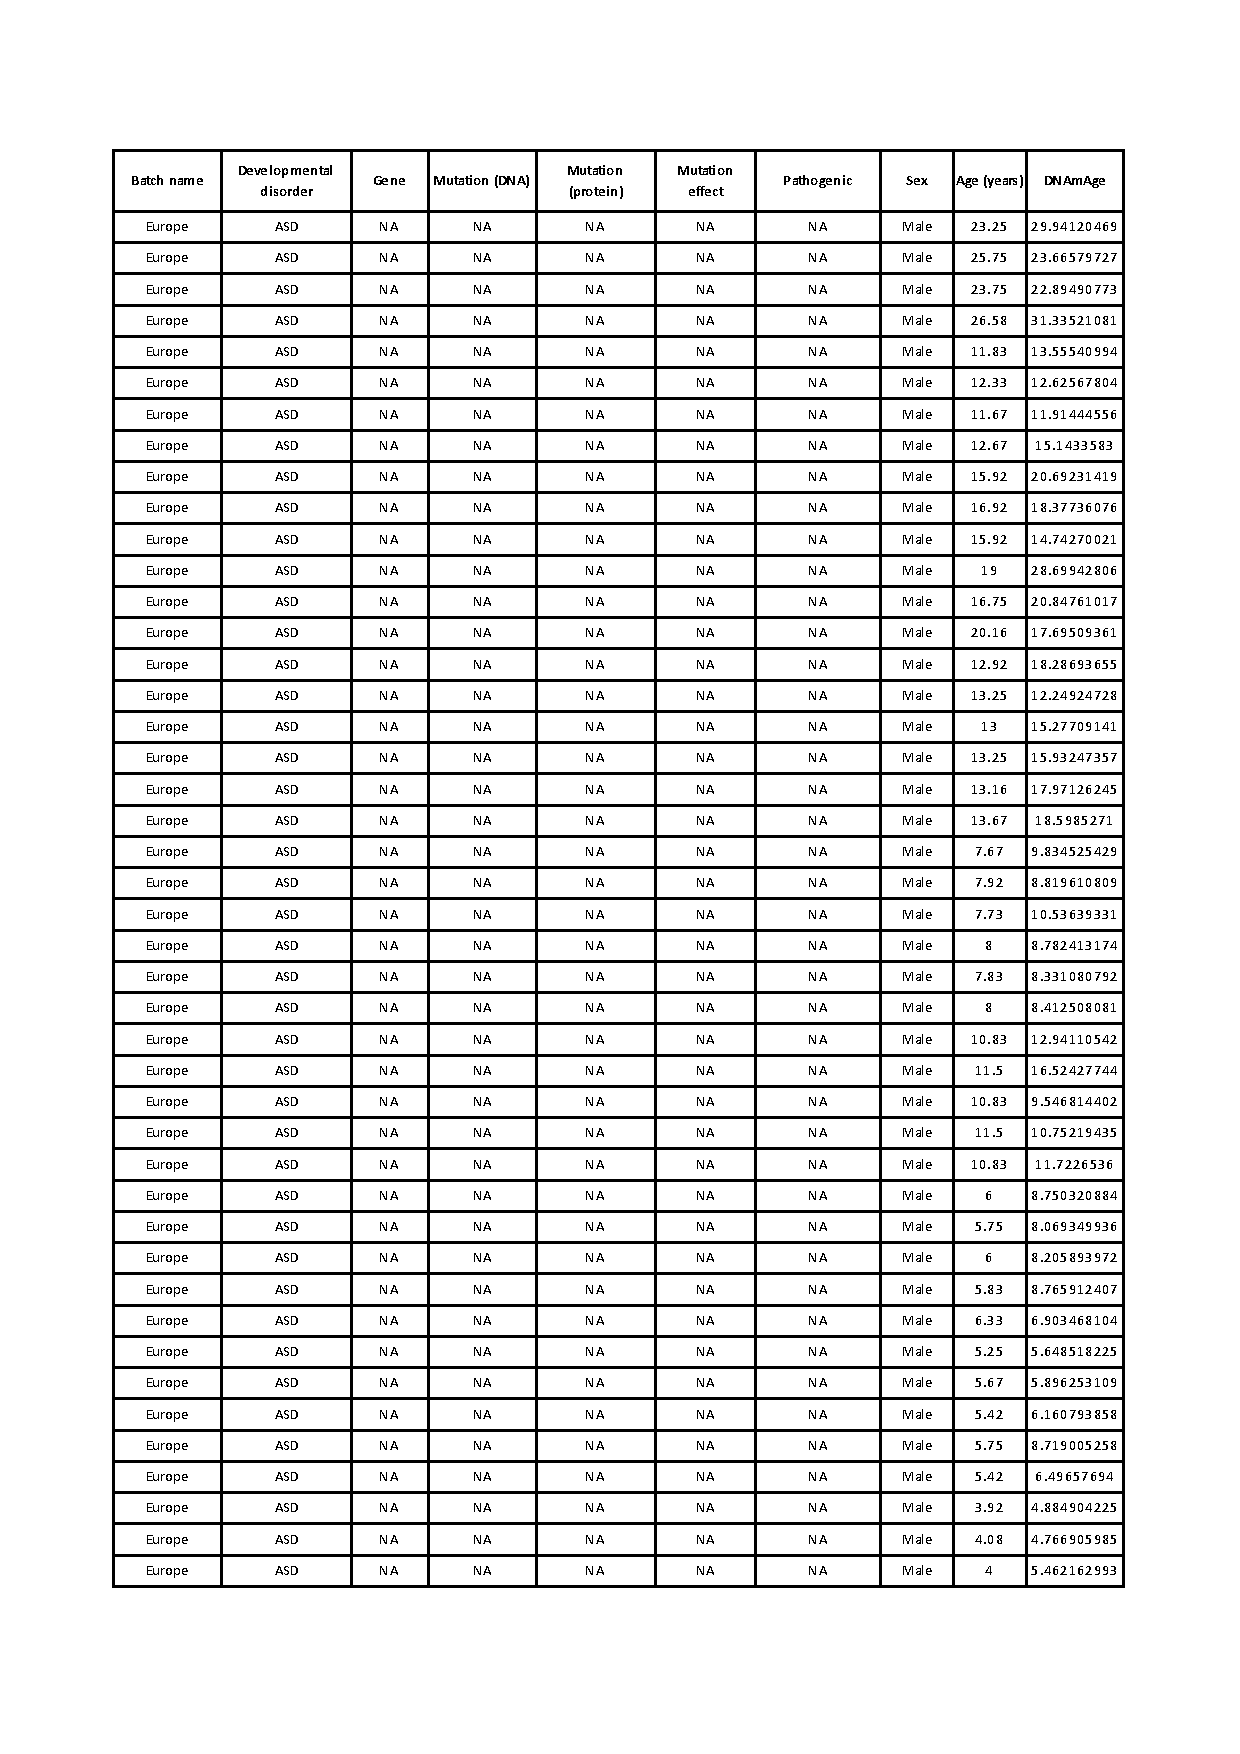
\includegraphics[width=1\textwidth]{SC3_Fig1_1}
\end{figure}
\begin{figure}[htbp!]
	\centering    
	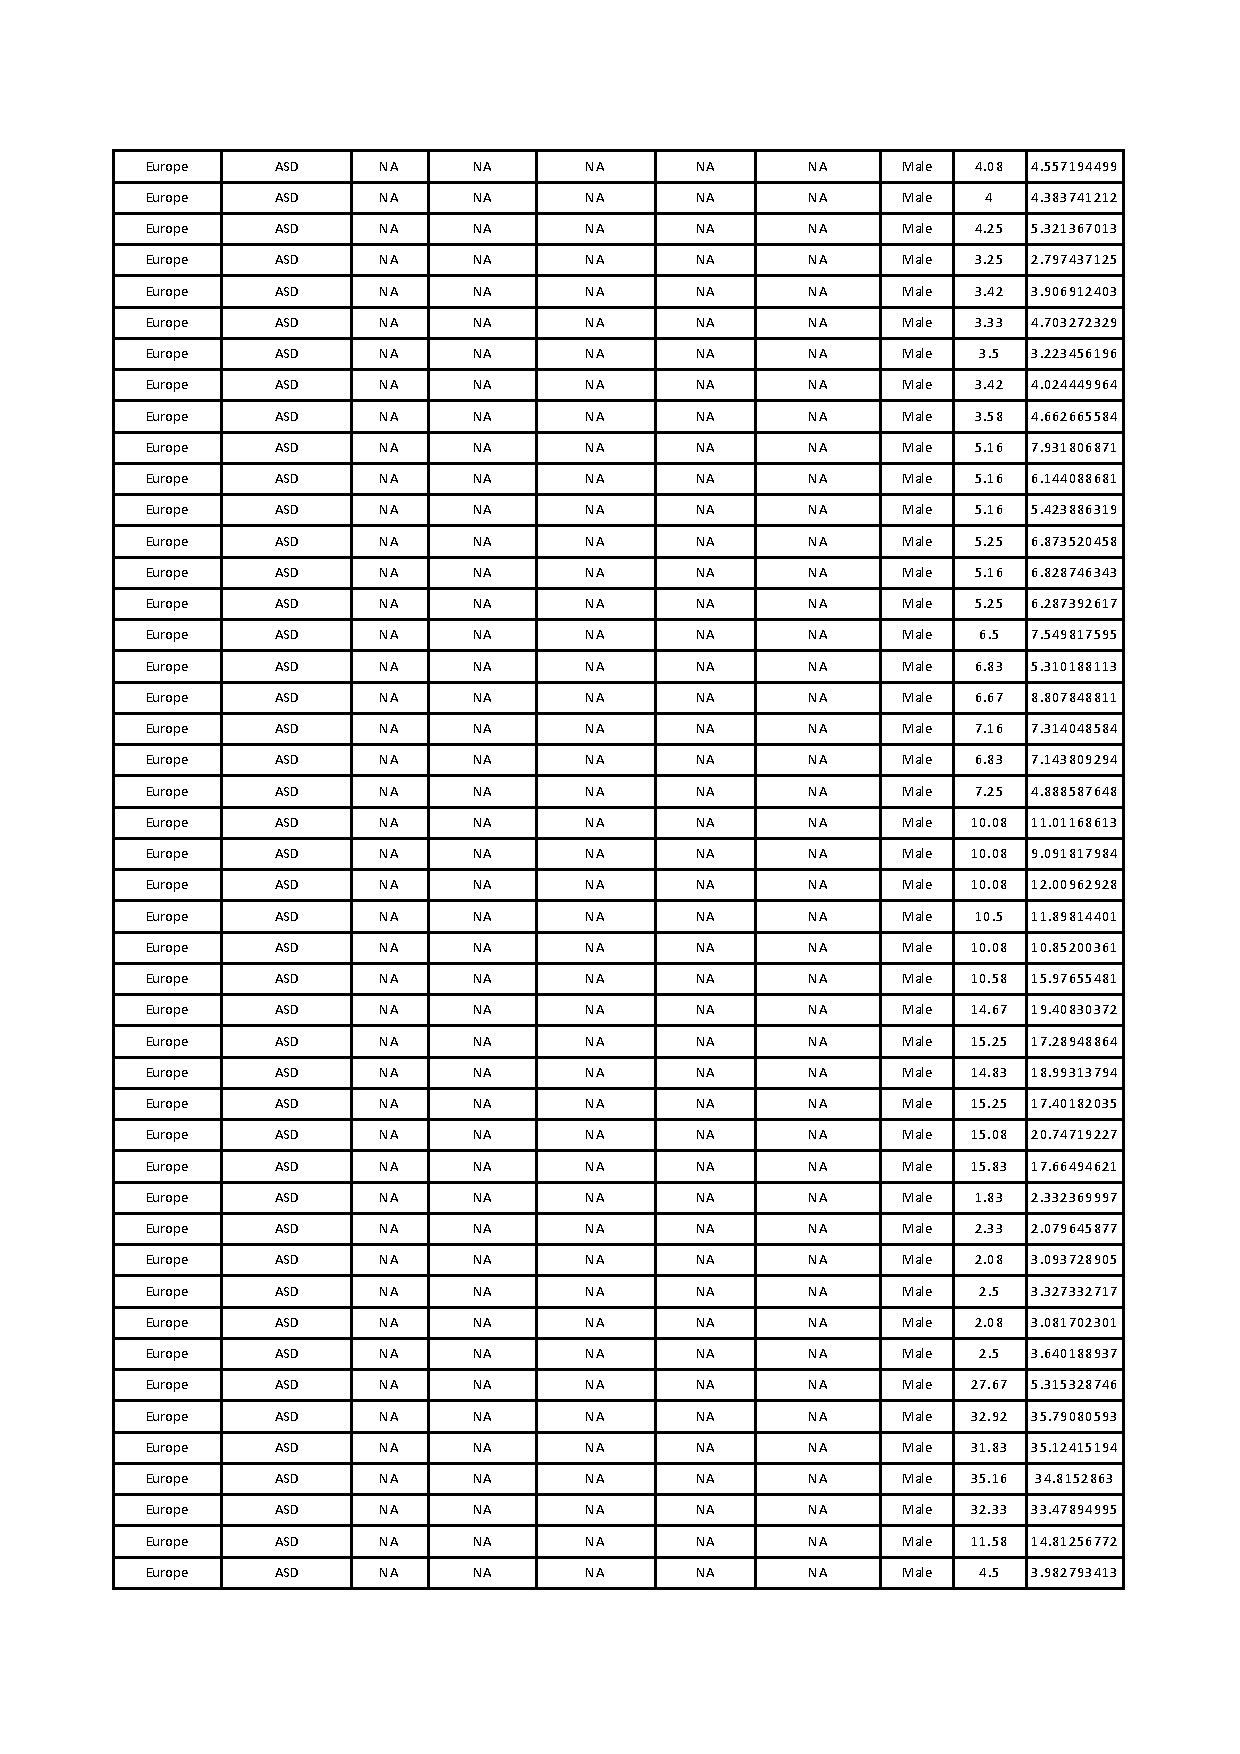
\includegraphics[width=1\textwidth]{SC3_Fig1_2}
\end{figure}
\begin{figure}[htbp!]
	\centering    
	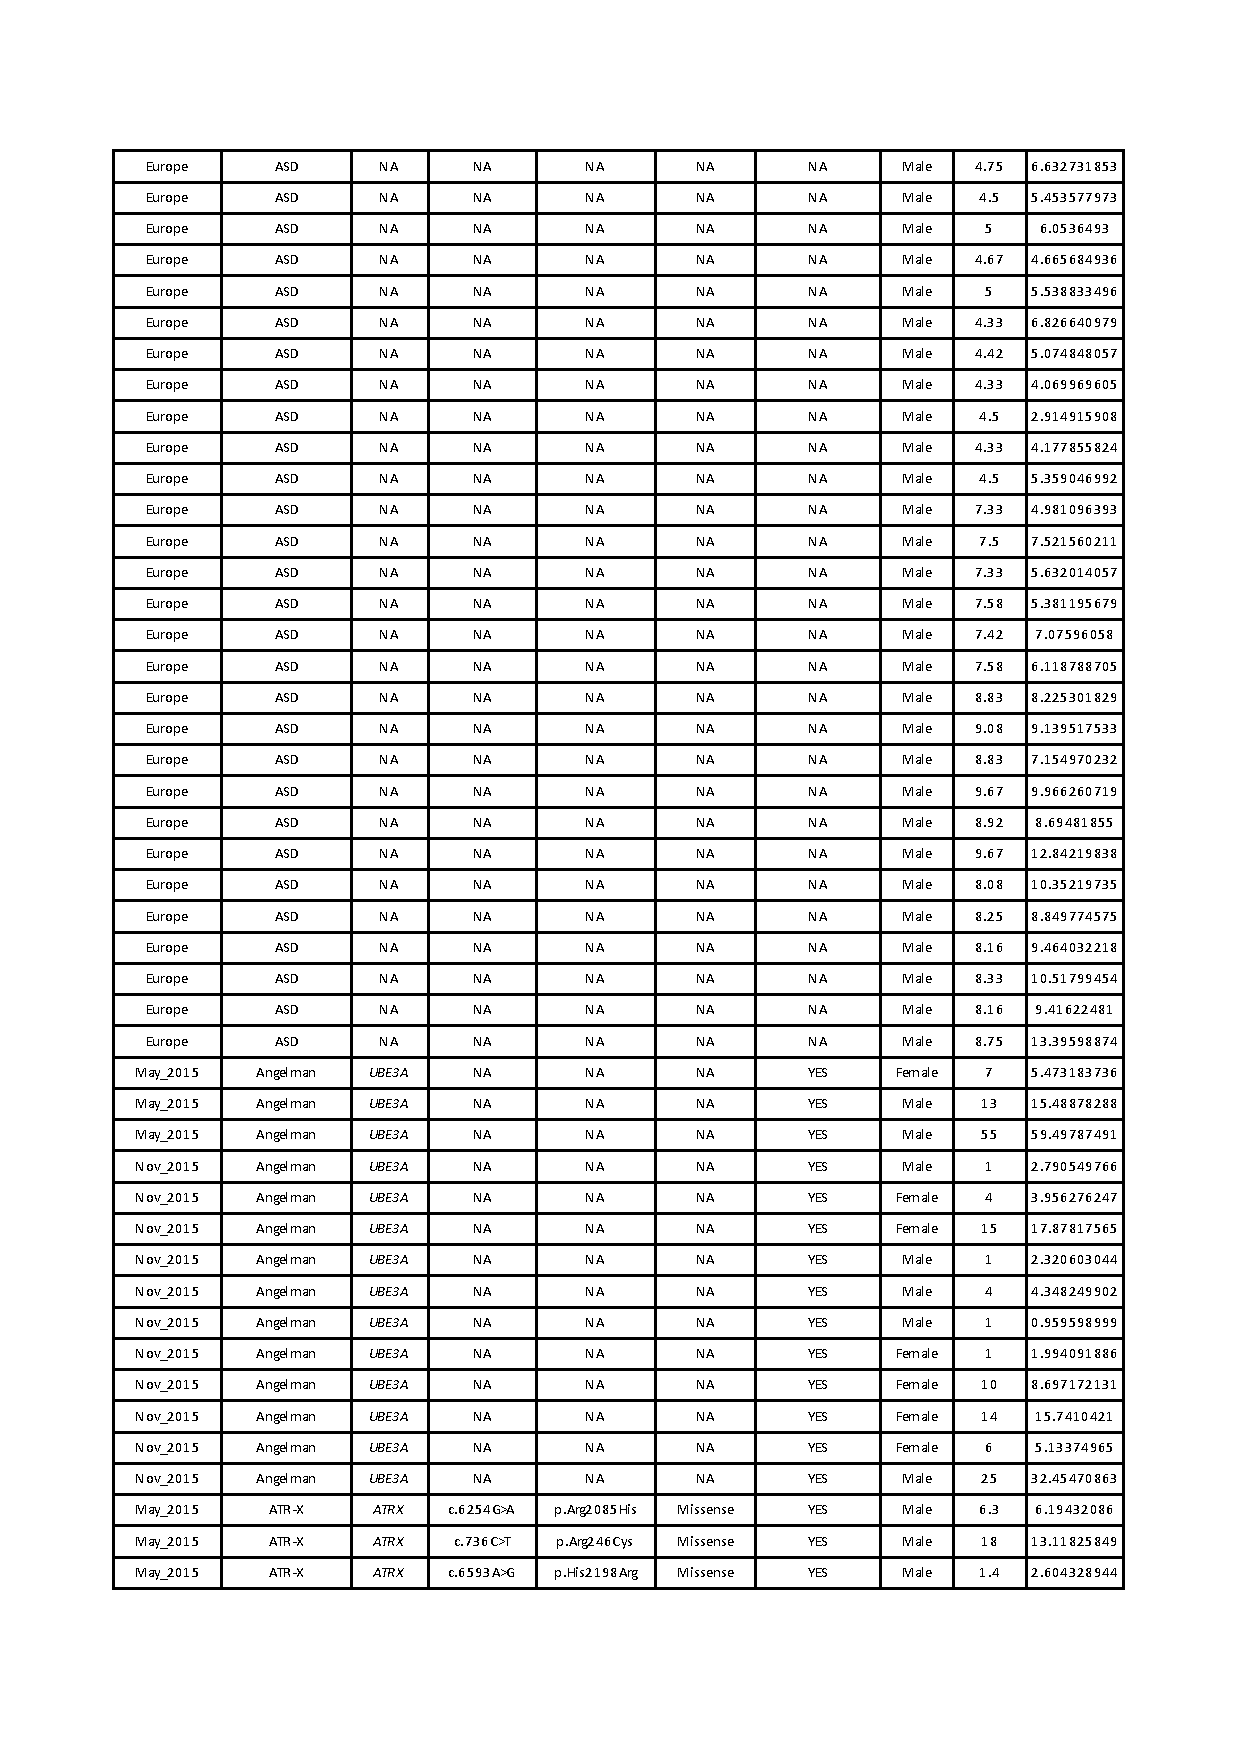
\includegraphics[width=1\textwidth]{SC3_Fig1_3}
\end{figure}
\begin{figure}[htbp!]
	\centering    
	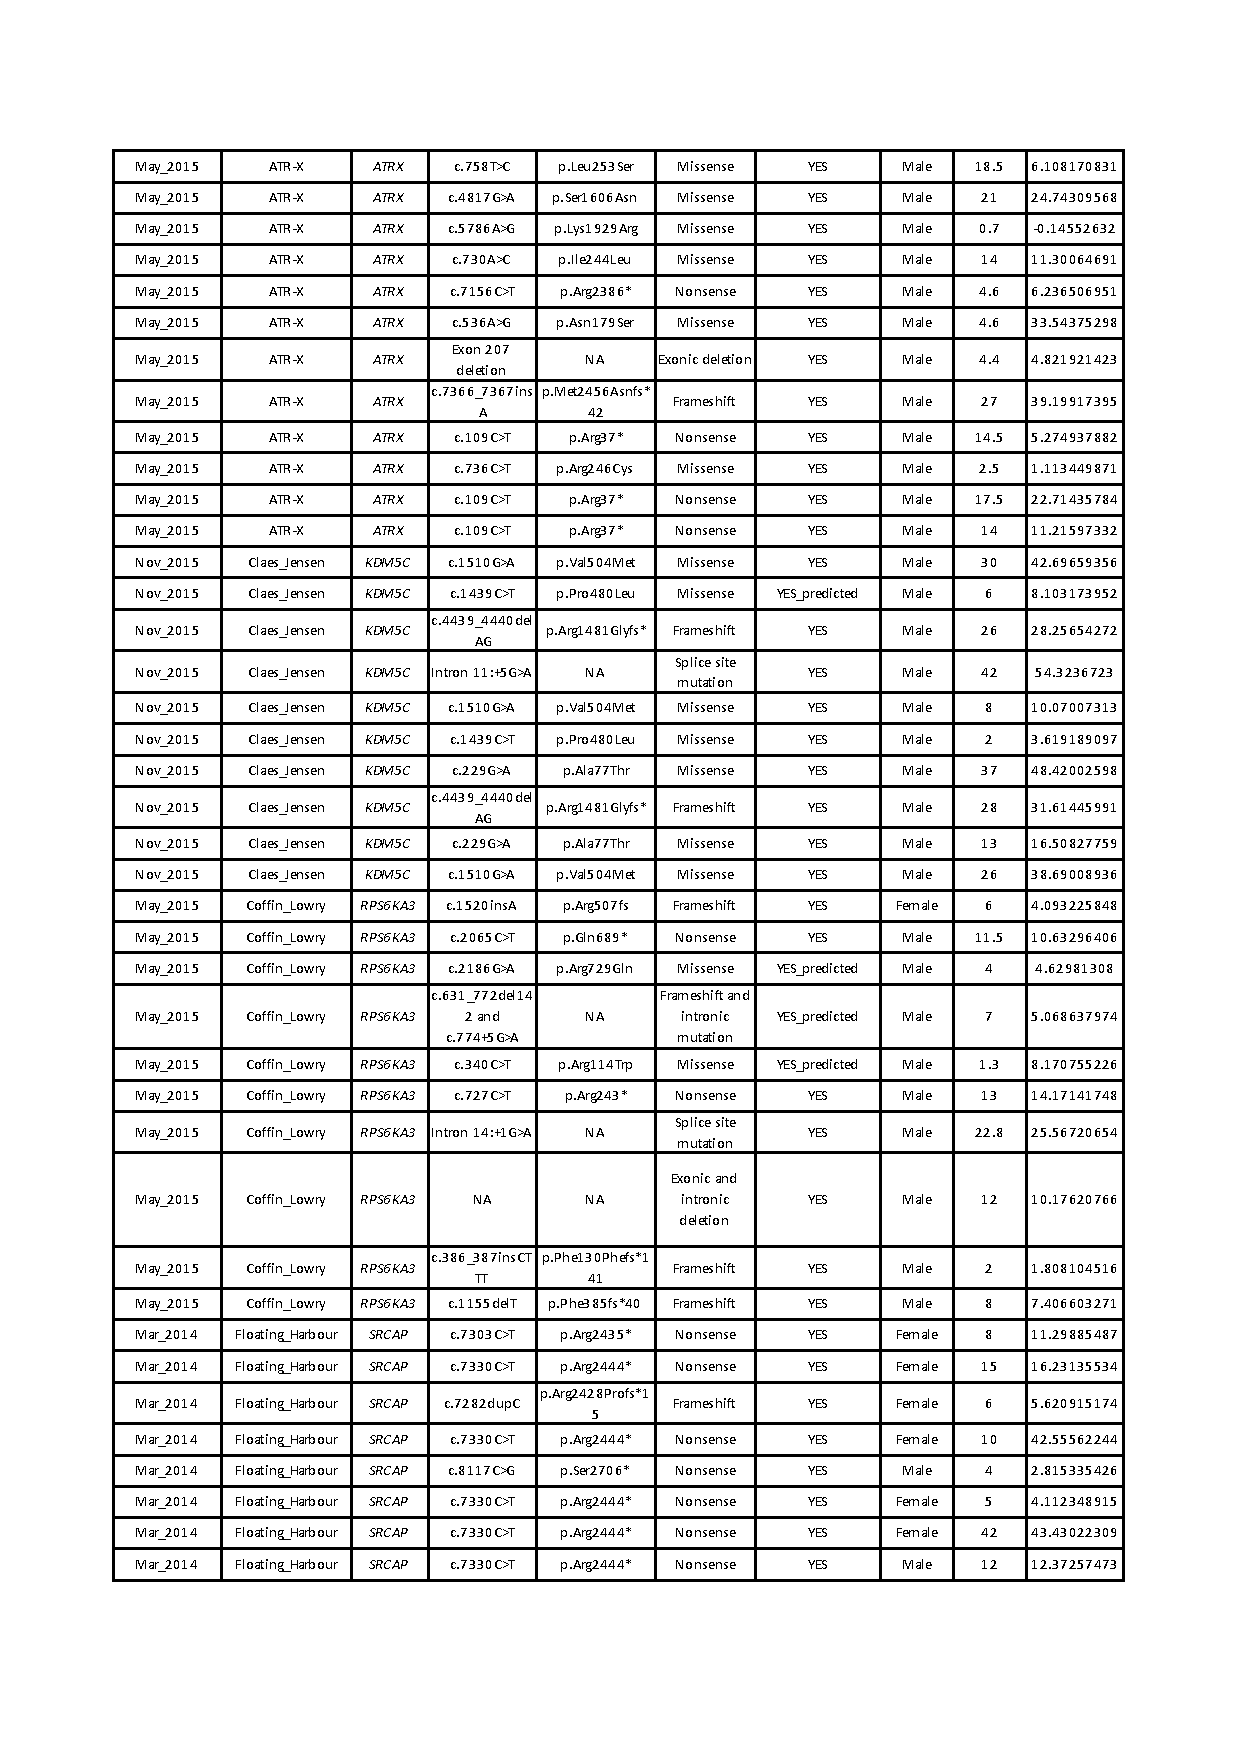
\includegraphics[width=1\textwidth]{SC3_Fig1_4}
\end{figure}
\begin{figure}[htbp!]
	\centering    
	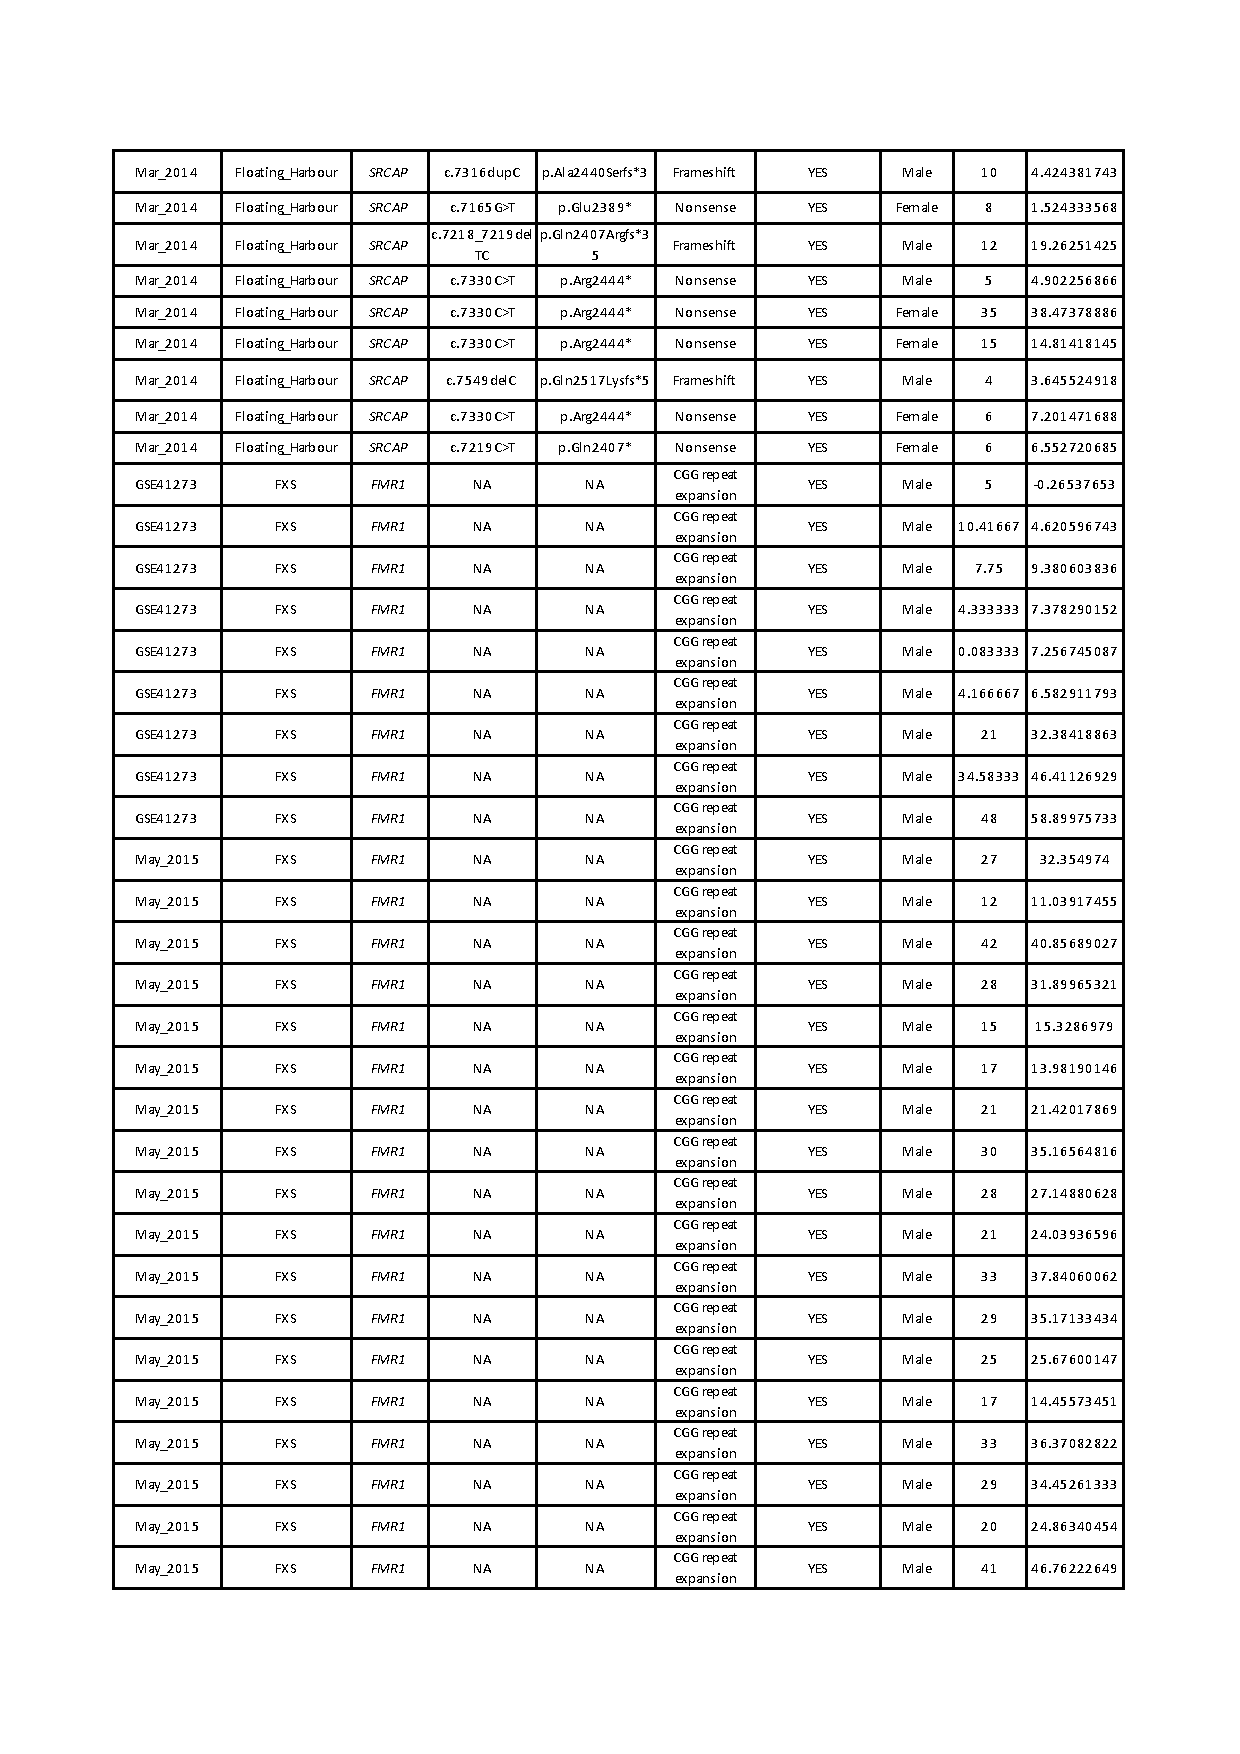
\includegraphics[width=1\textwidth]{SC3_Fig1_5}
\end{figure}
\begin{figure}[htbp!]
	\centering    
	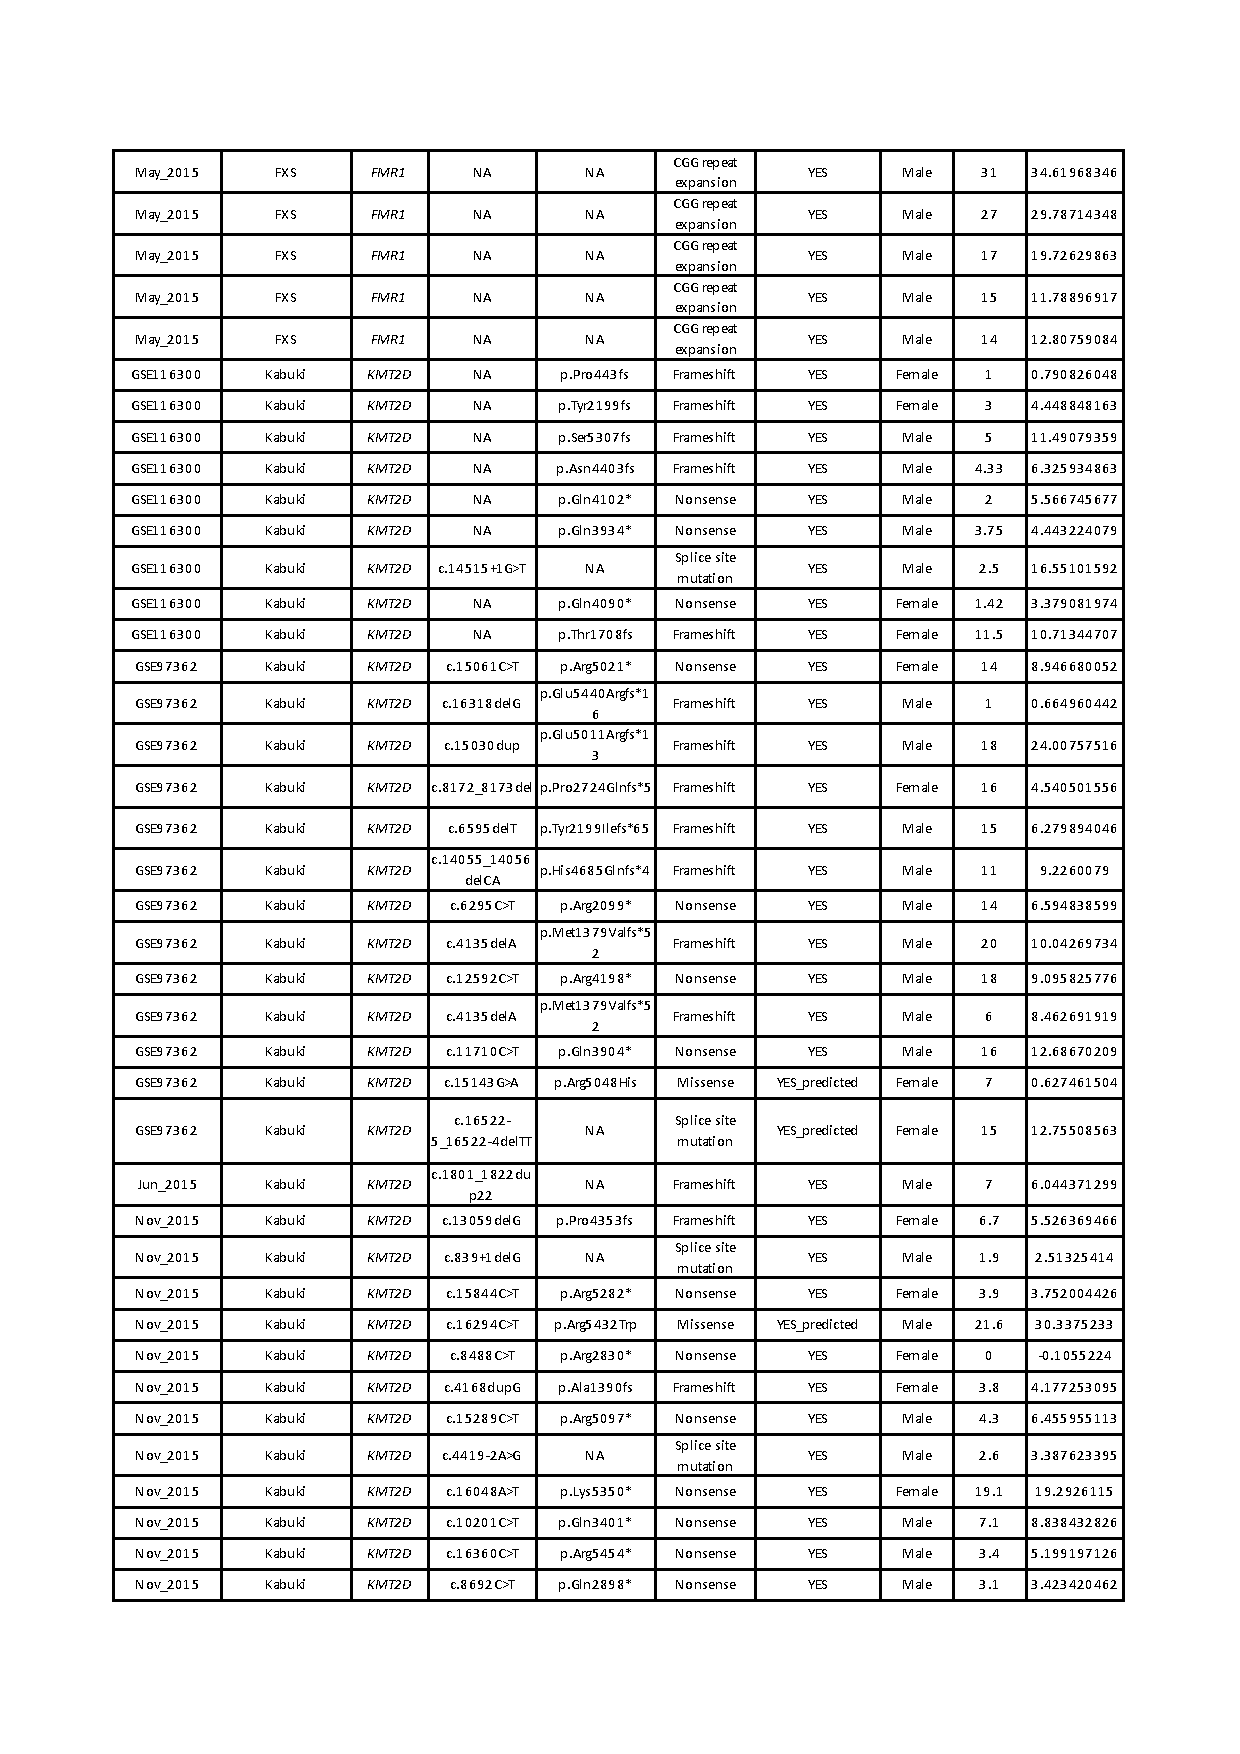
\includegraphics[width=1\textwidth]{SC3_Fig1_6}
\end{figure}
\begin{figure}[htbp!]
	\centering    
	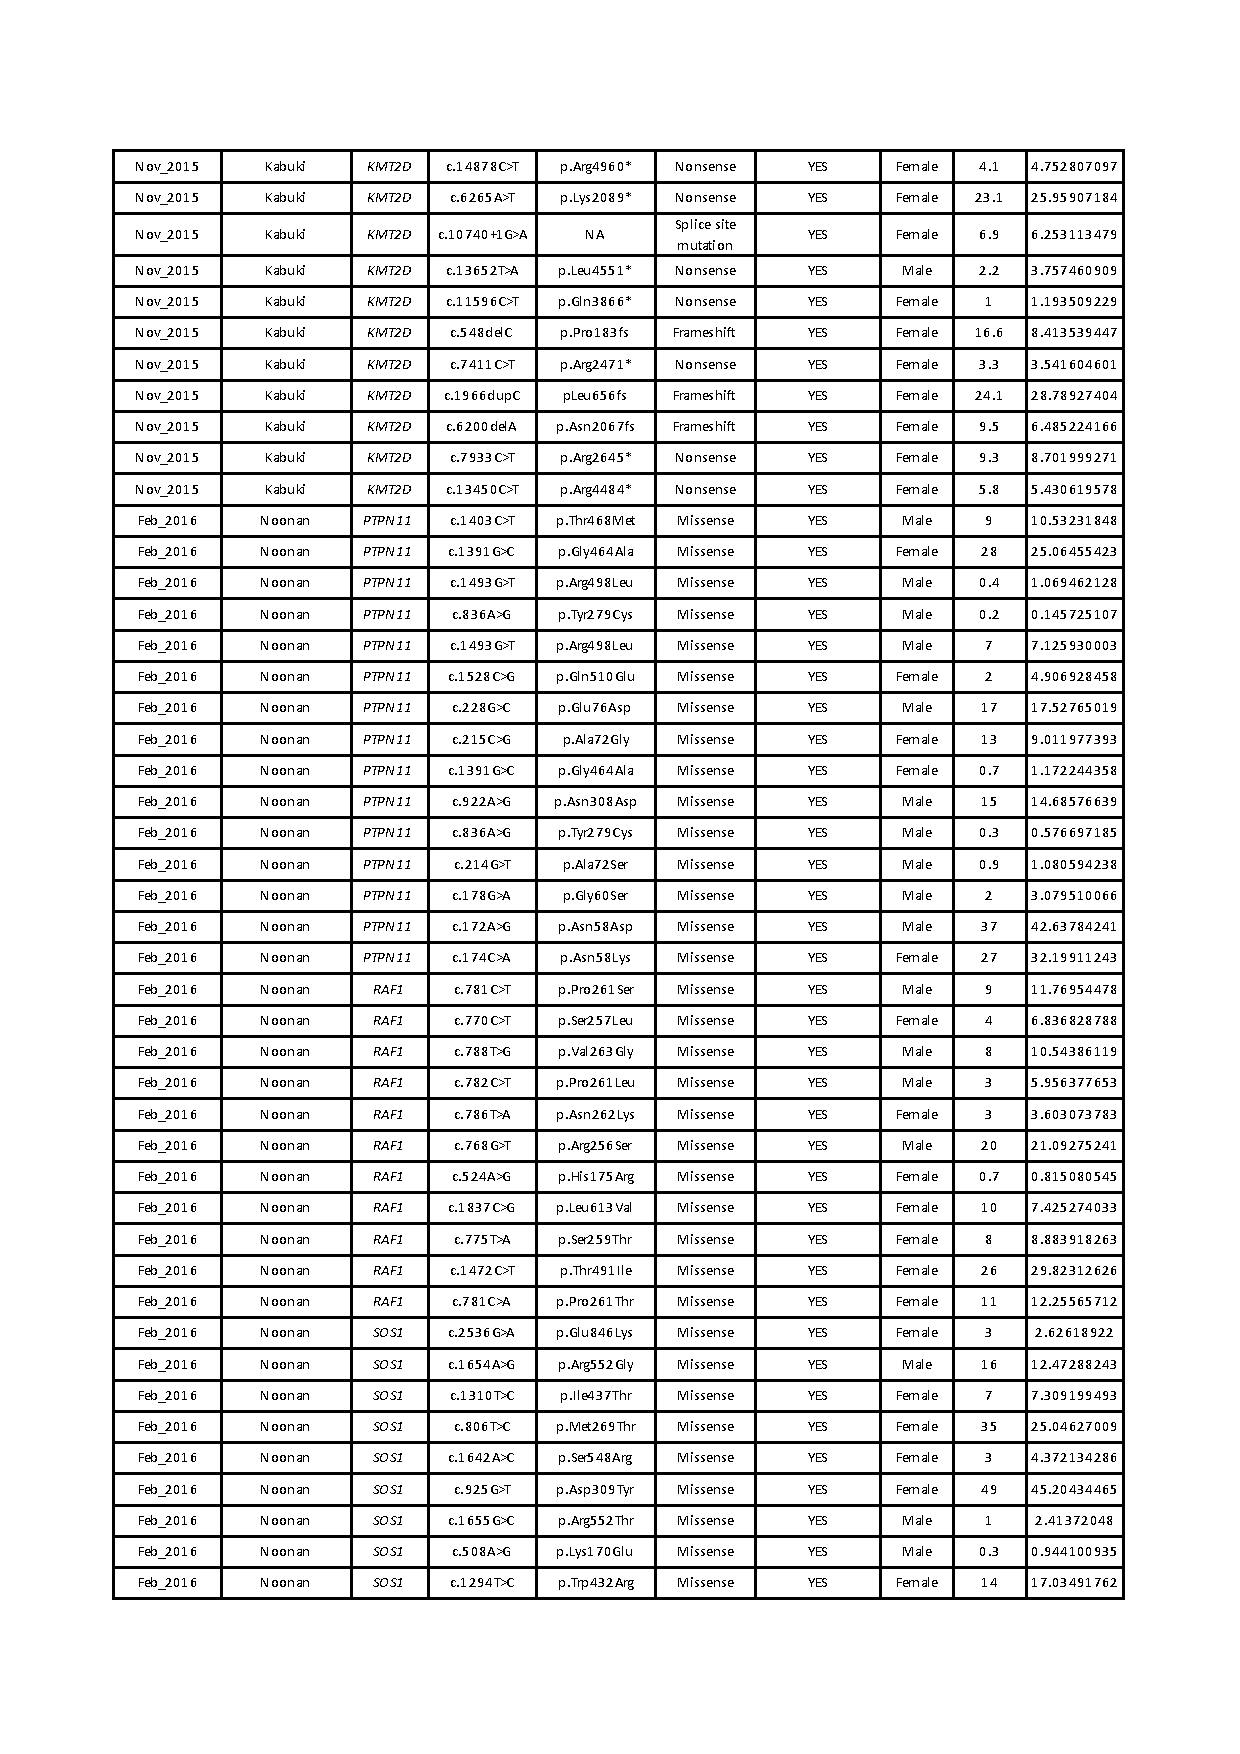
\includegraphics[width=1\textwidth]{SC3_Fig1_7}
\end{figure}
\begin{figure}[htbp!]
	\centering    
	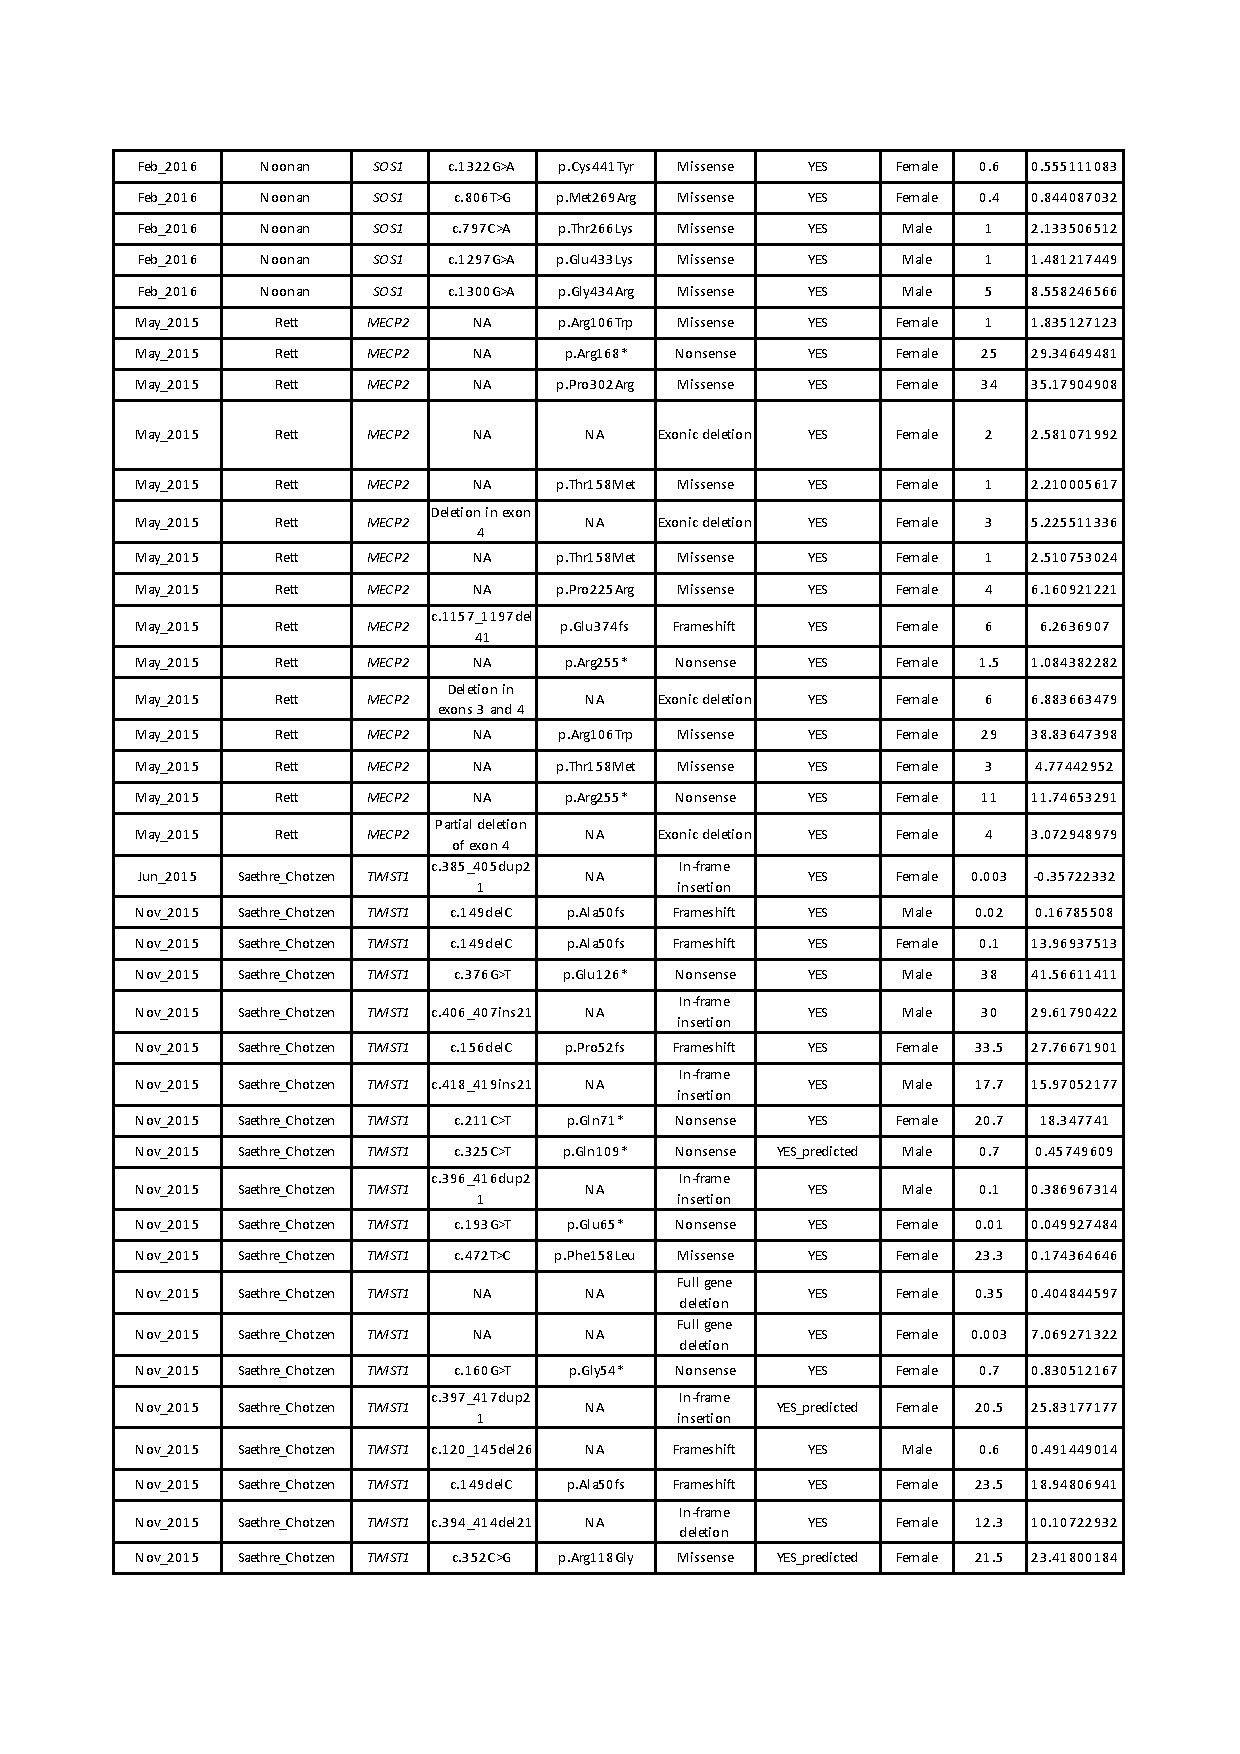
\includegraphics[width=1\textwidth]{SC3_Fig1_8}
\end{figure}
\begin{figure}[htbp!]
	\centering
	\vspace*{-40mm}    
	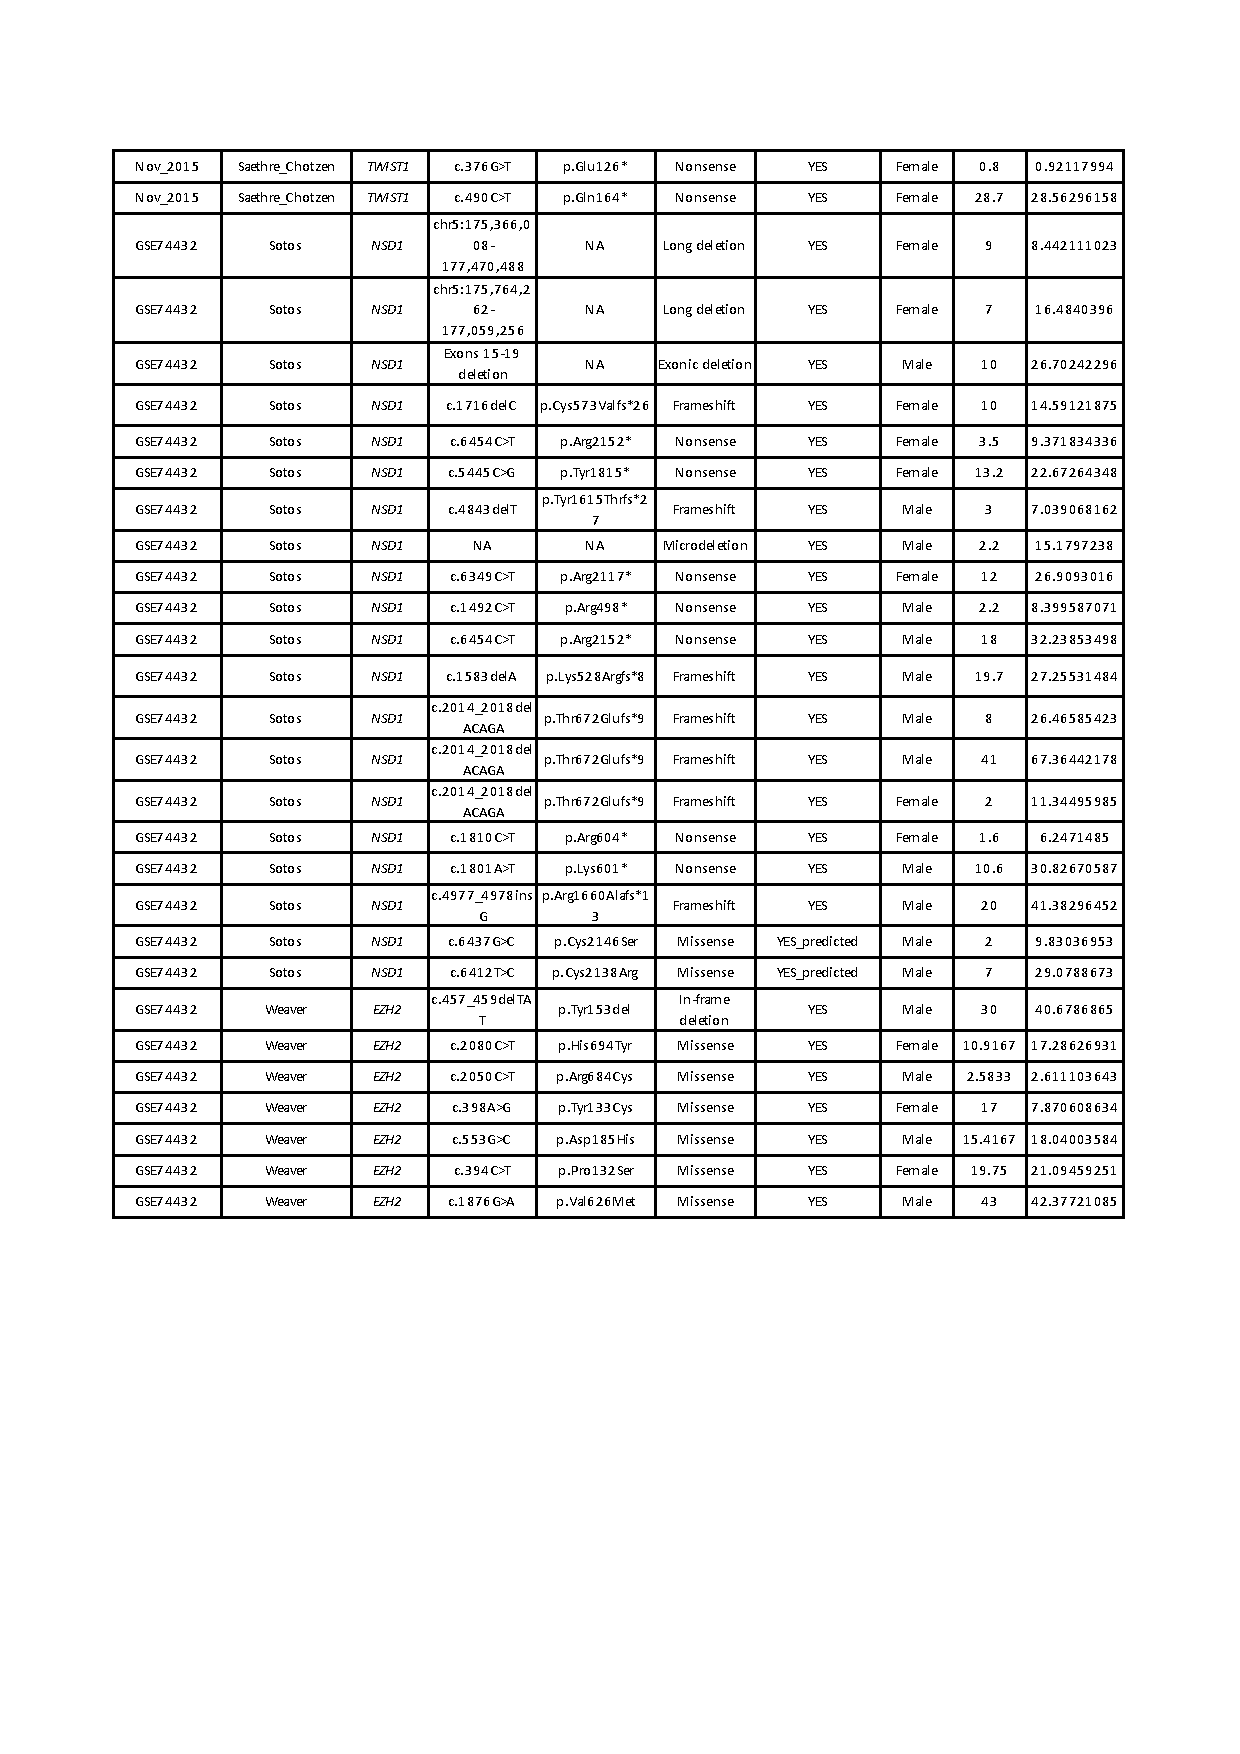
\includegraphics[width=1\textwidth]{SC3_Fig1_9}
	\caption[Table showing information for the individuals with developmental disorders]{Table showing information for the samples from individuals with developmental disorders (total $N=367$). Mutation information was annotated for the human genome assembly \textit{hg19}. \acrshort{ASD}: autism spectrum disorder; \acrshort{ATR-X}: alpha thalassemia/mental retardation X-linked syndrome; \acrshort{FXS}: fragile X syndrome.}
	\label{fig:sc3_fig1}
\end{figure}	

\begin{figure}[htbp!] 
	\centering    
	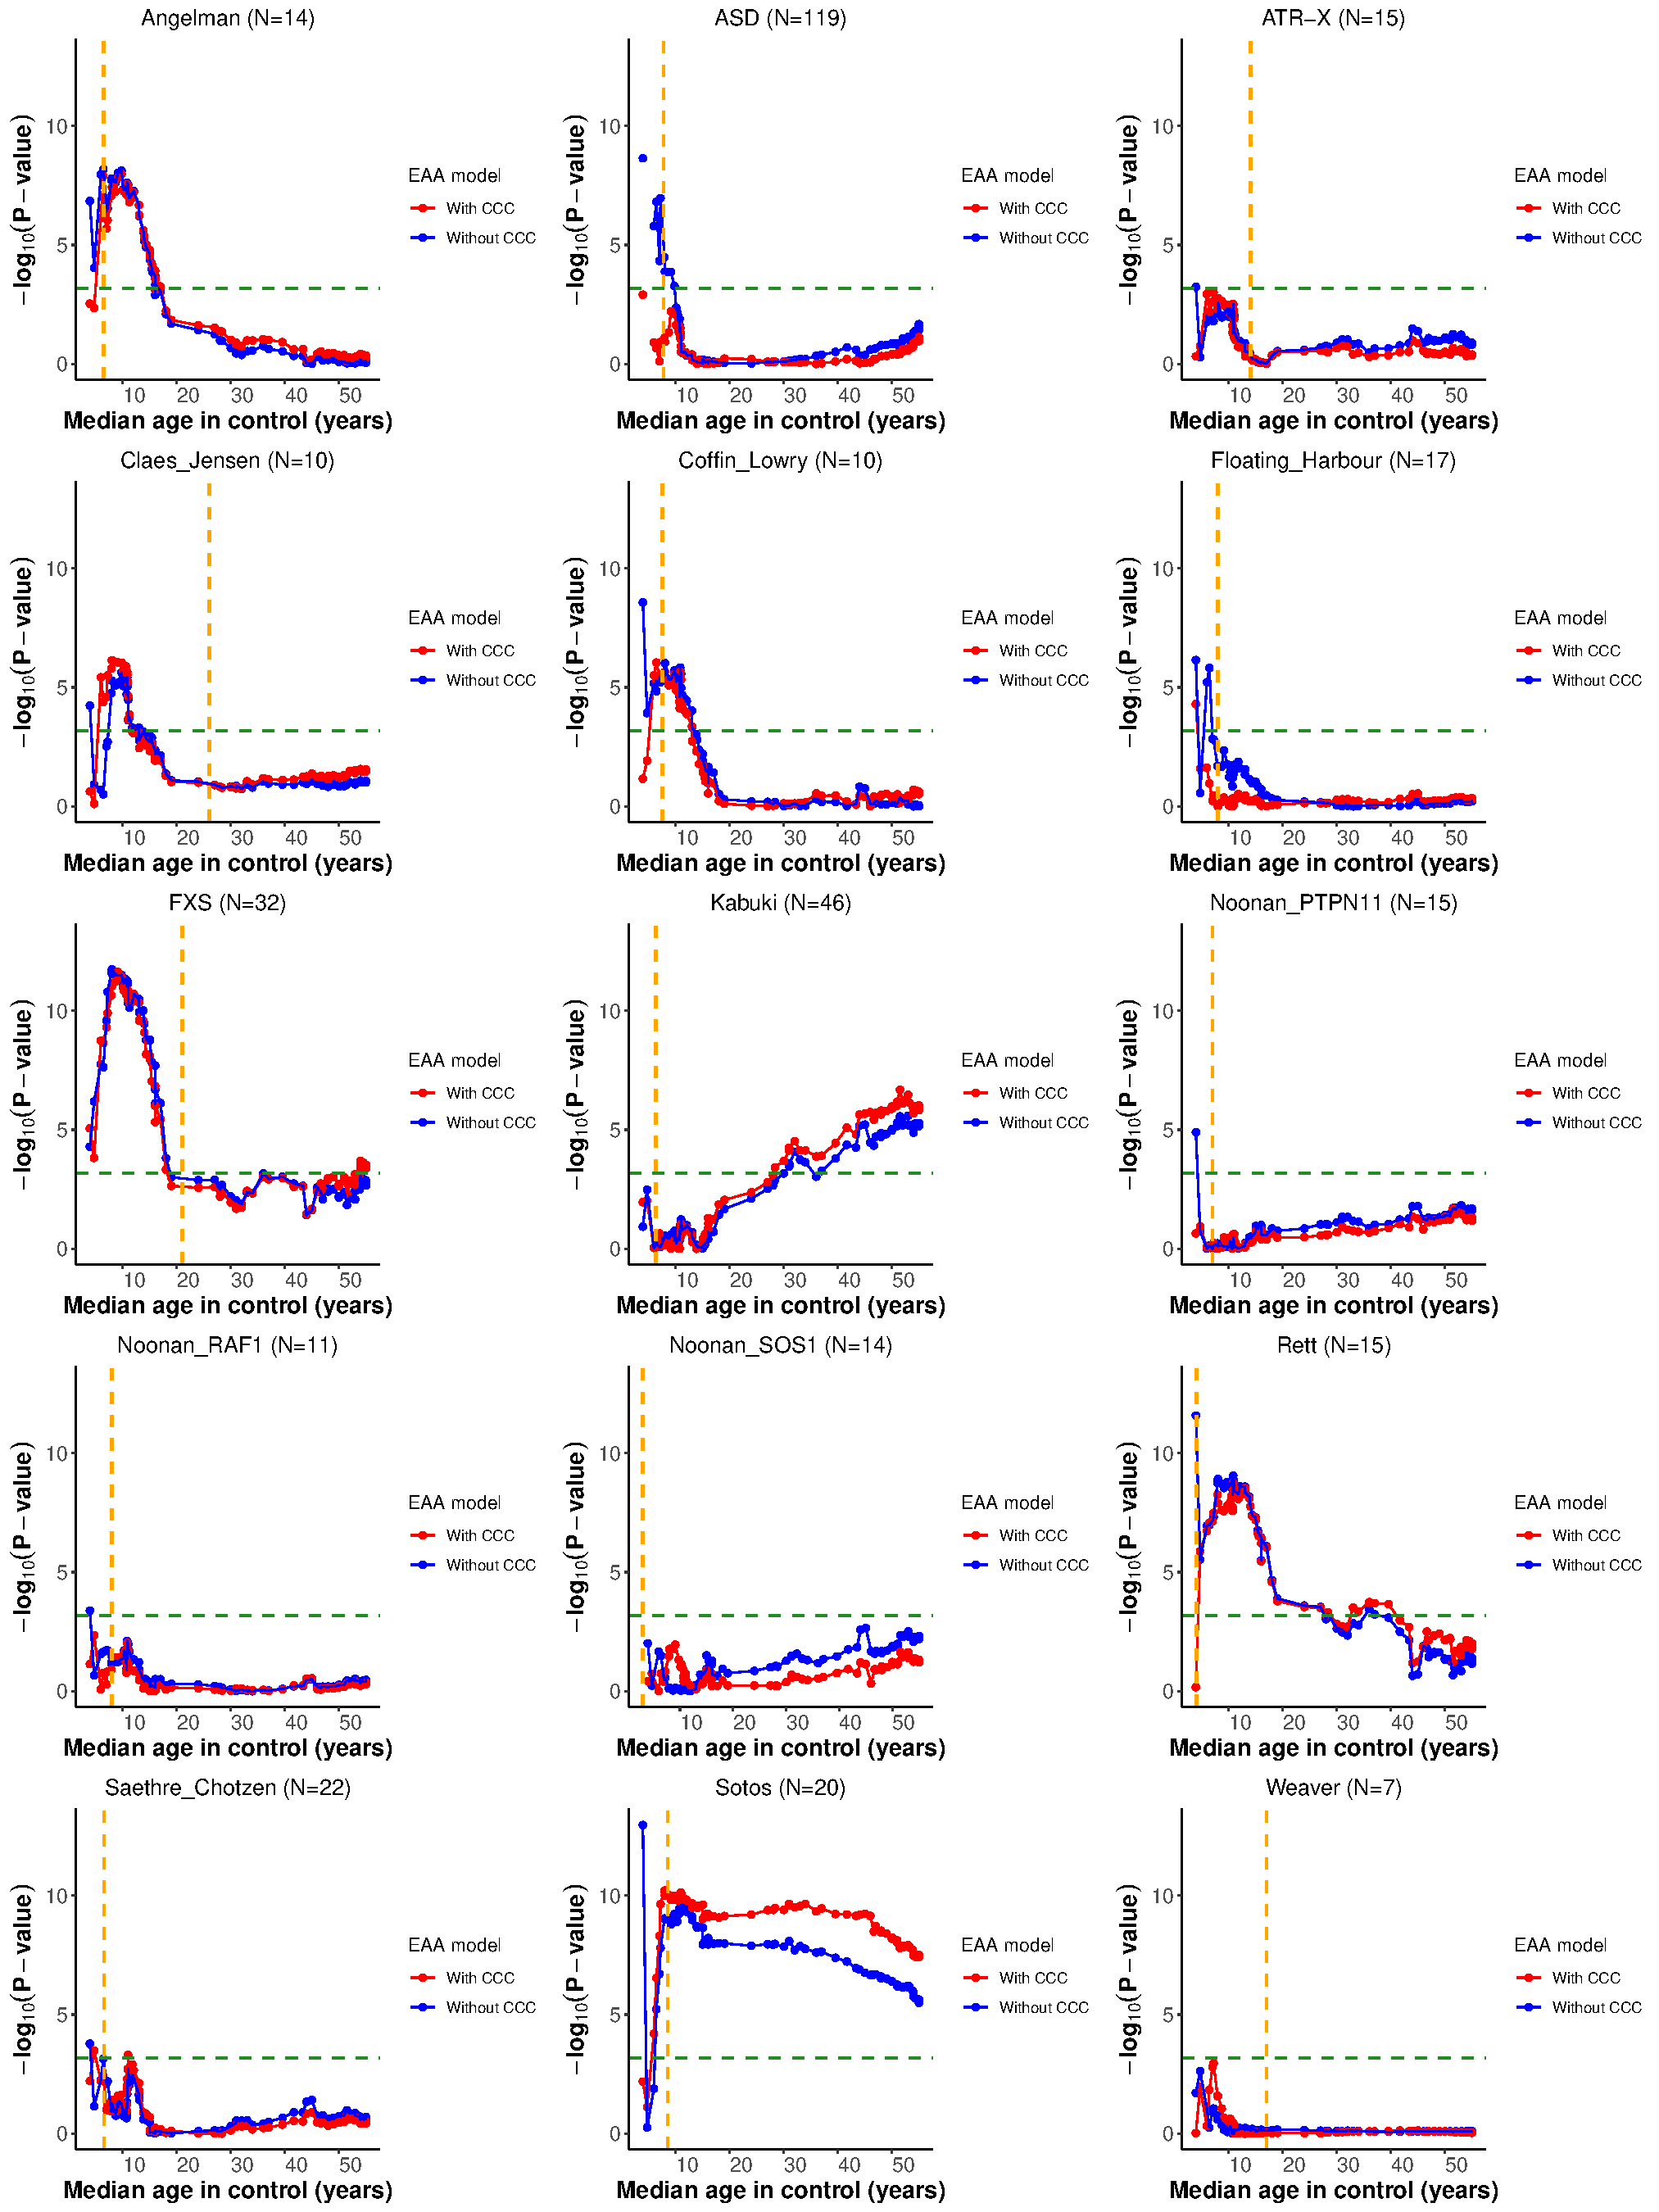
\includegraphics[width=1\textwidth]{SC3_Fig2}
	\caption[Effect of changing the median age of the controls when performing the screening]{Effect of changing the median age of the controls when performing the screening for epigenetic age acceleration (EAA) in the different developmental disorders. The dashed green line displays the significance level of $\alpha = 0.01$ after Bonferroni correction. The dashed orange line displays the median age for the samples in the developmental disorder considered. In blue: EAA model without cell composition correction (CCC). In red: EAA model with CCC. \acrshort{ASD}: autism spectrum disorder; \acrshort{ATR-X}: alpha thalassemia/mental retardation X-linked syndrome; \acrshort{FXS}: fragile X syndrome.}
	\label{fig:sc3_fig2}
\end{figure}

\begin{figure}[htbp!]
	\centering    
	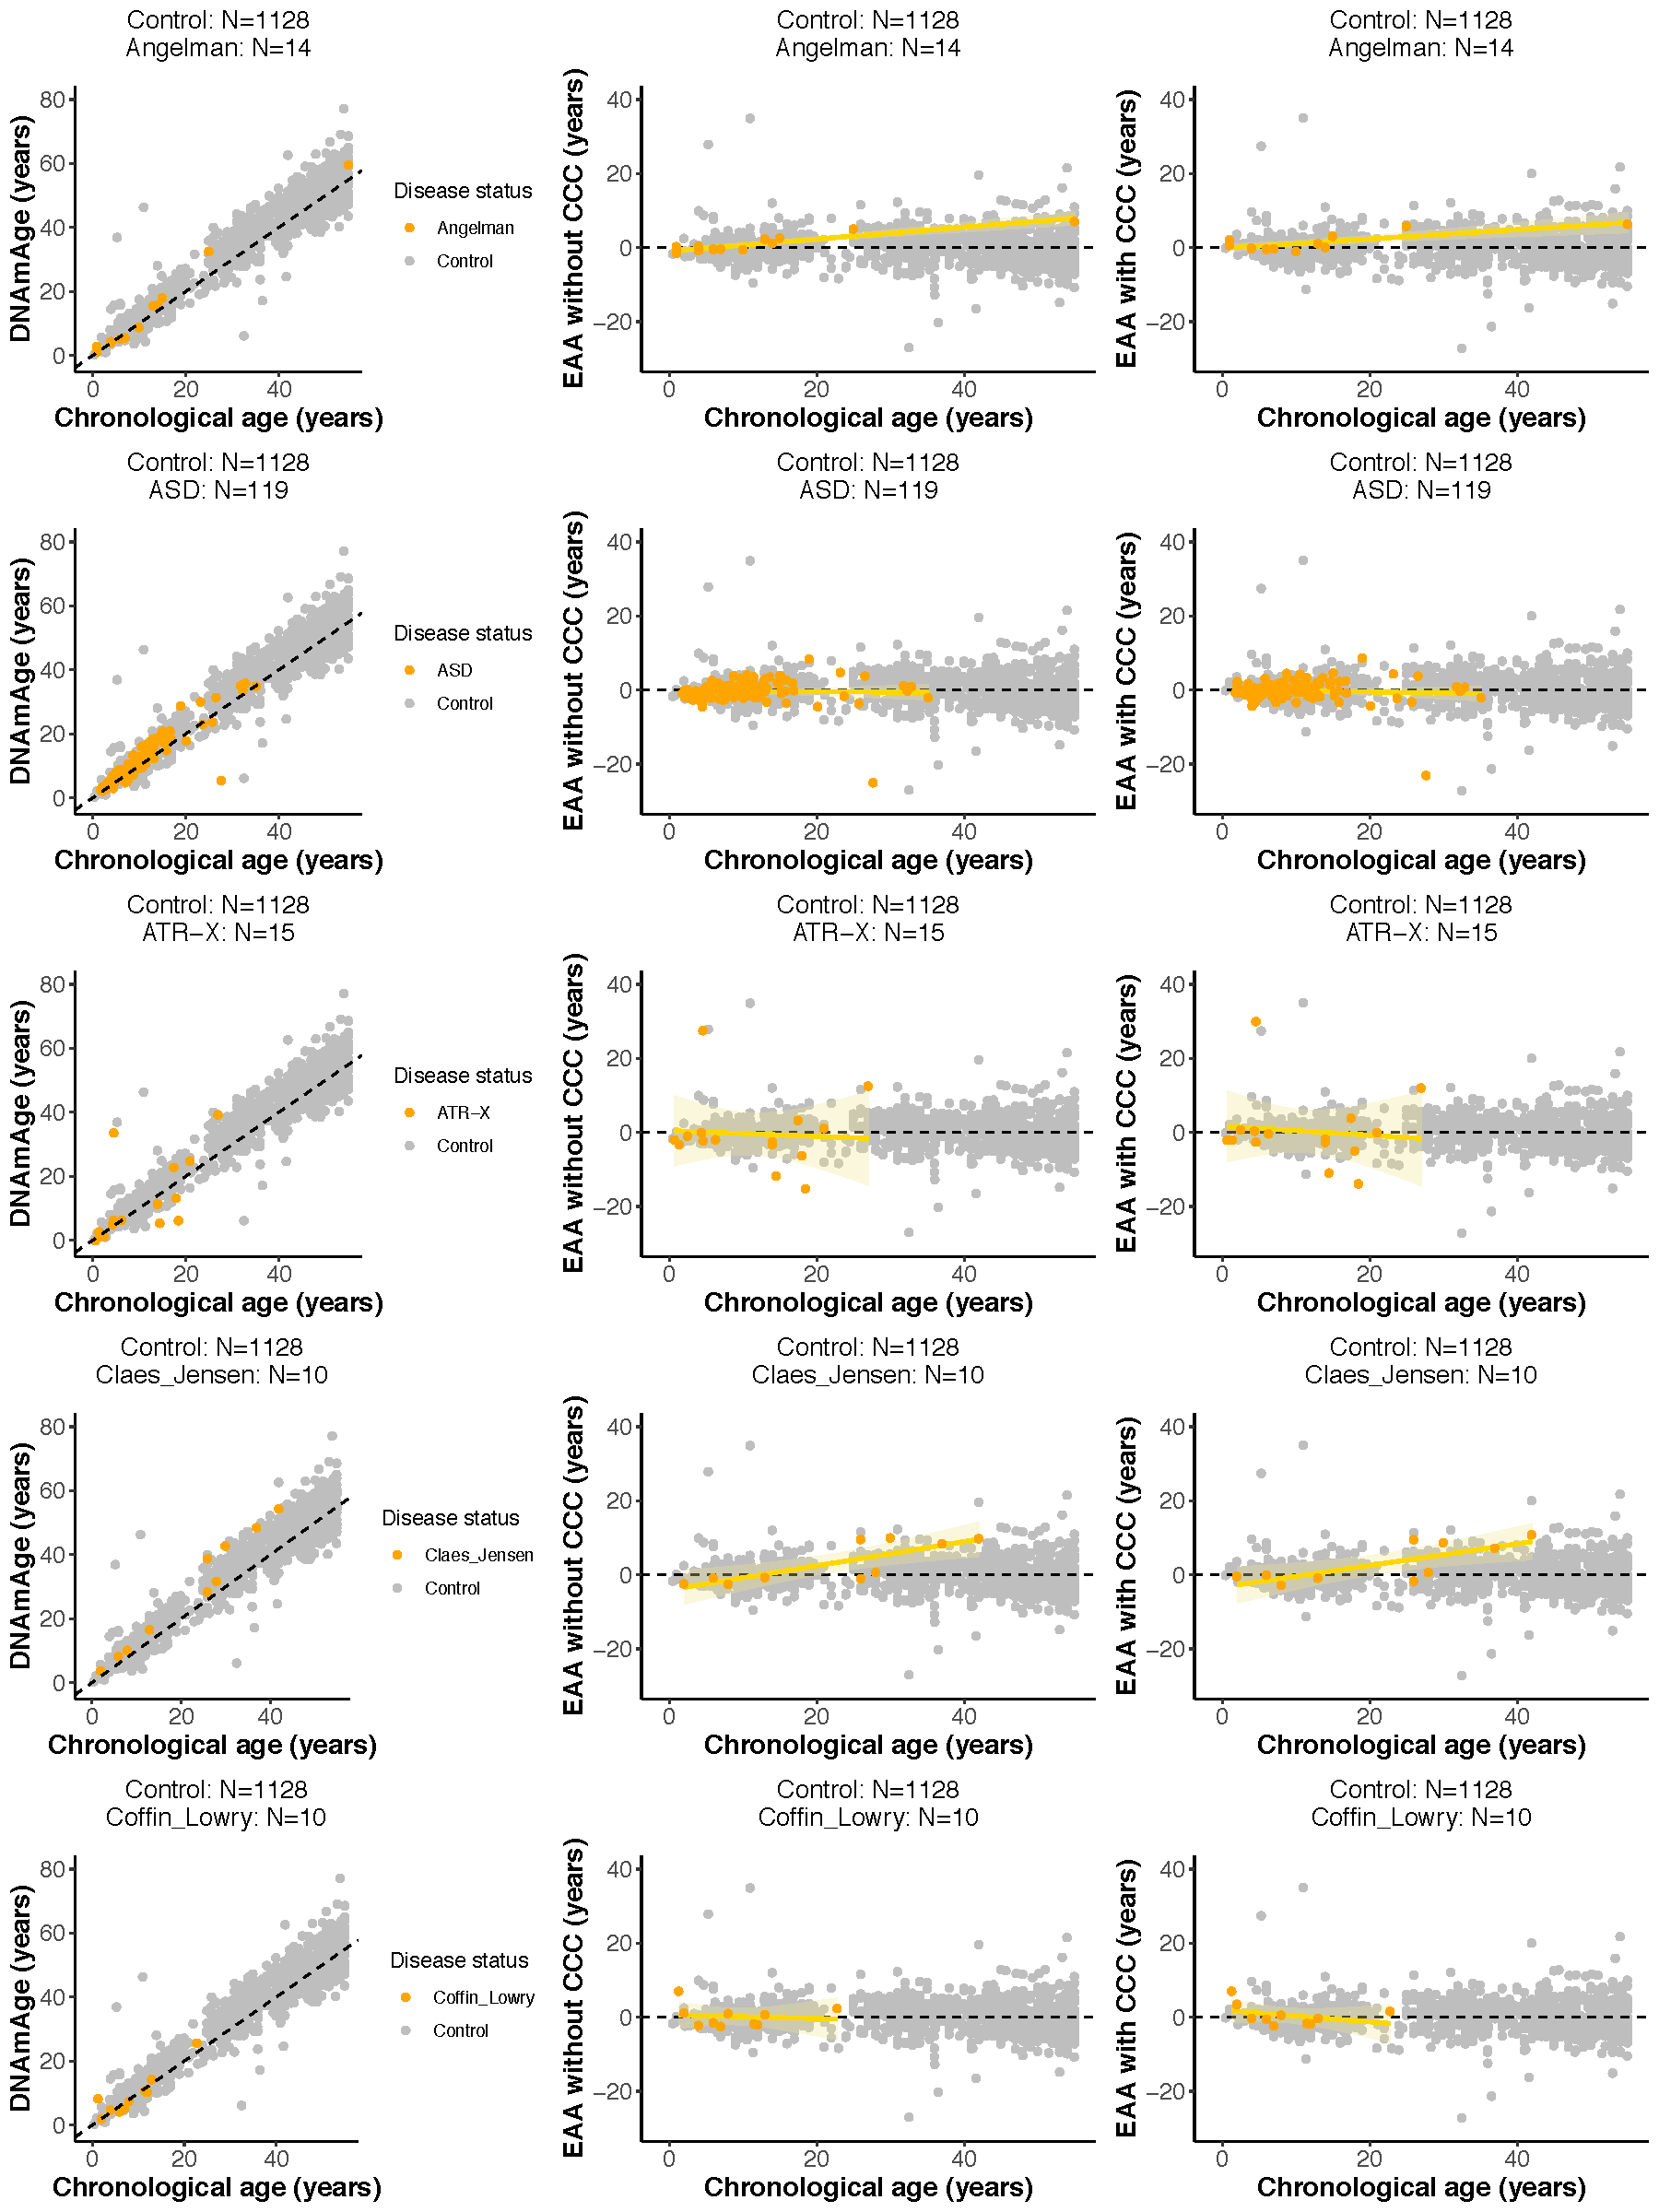
\includegraphics[width=1\textwidth]{SC3_Fig3_1}
\end{figure}
\begin{figure}[htbp!]
	\centering    
	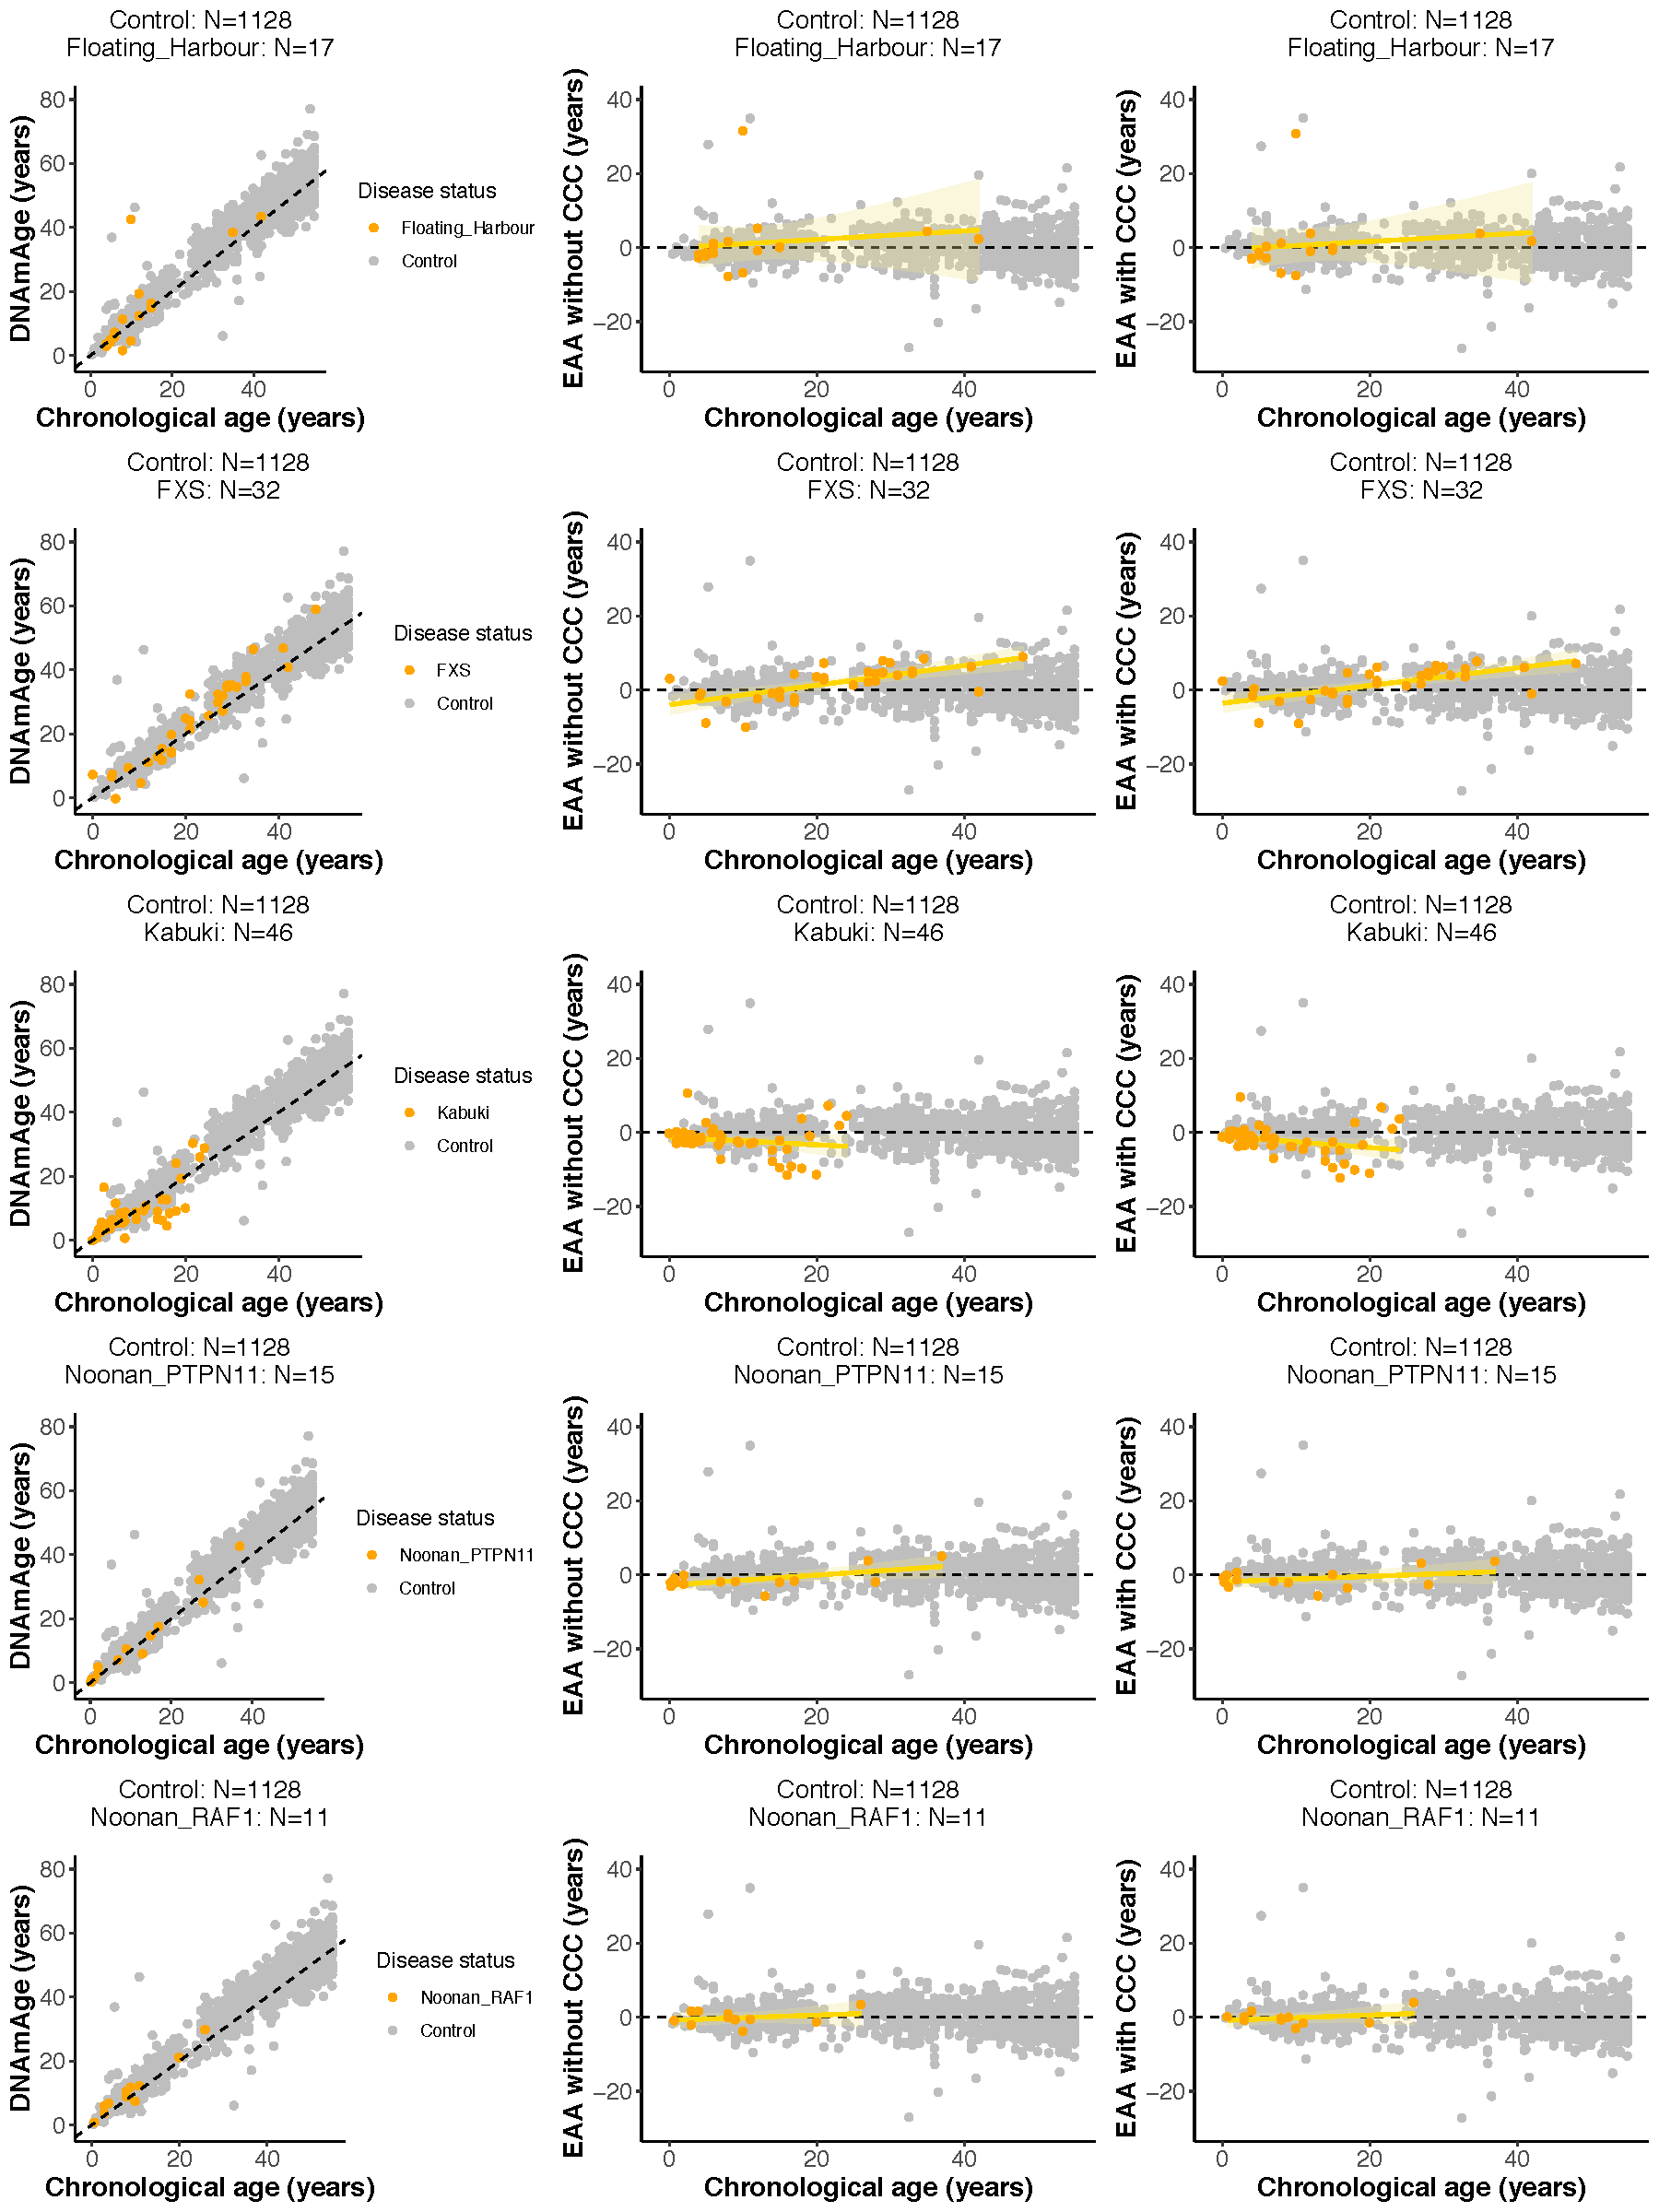
\includegraphics[width=1\textwidth]{SC3_Fig3_2}
\end{figure}
\begin{figure}[htbp!]
	\centering
	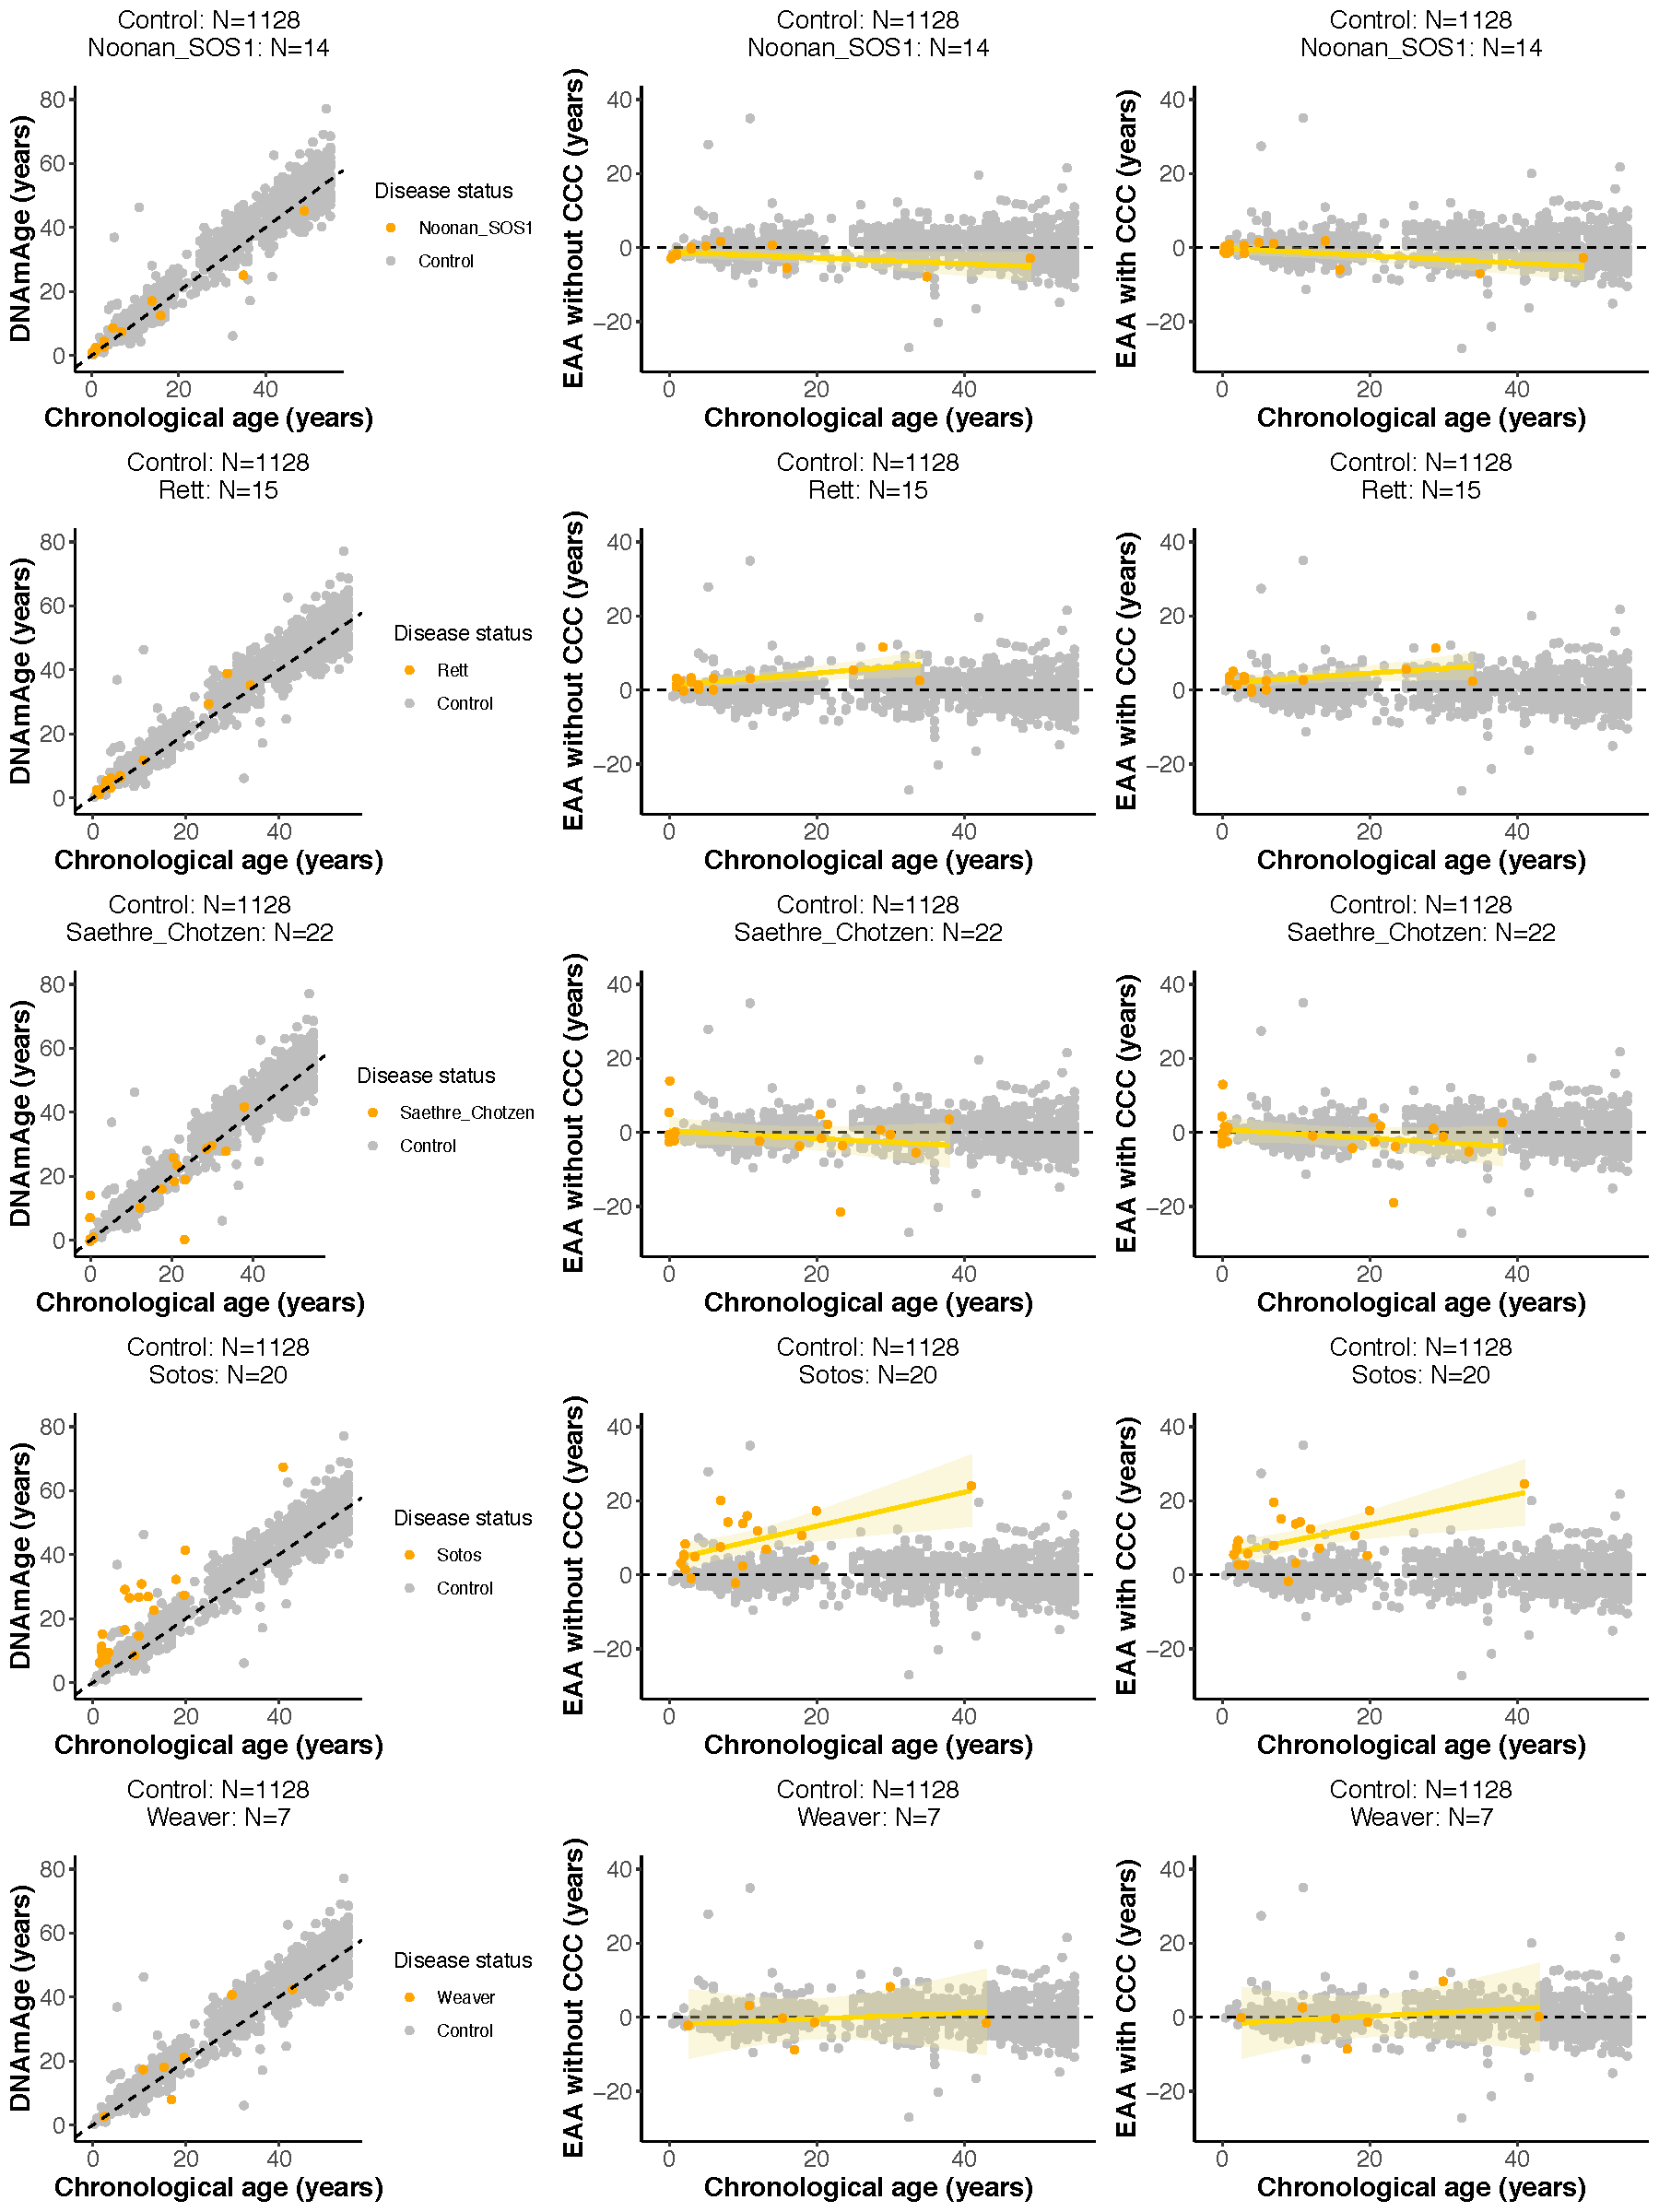
\includegraphics[width=1\textwidth]{SC3_Fig3_3}
	\caption[Screening for epigenetic age acceleration (EAA) in developmental disorders: additional scatterplots]{Screening for epigenetic age acceleration (EAA) in developmental disorders. Left panel: scatterplot showing the relation between epigenetic age ($DNAmAge$) according to Horvath’s model and chronological age of the samples for a given developmental disorder (orange) and control (grey). Each sample is represented by one point. The black dashed line represents the diagonal to aid visualisation. Middle and right panels: scatterplots showing the relation between the epigenetic age acceleration (EAA) (without and with CCC respectively) and chronological age of the samples for a given developmental disorder (orange) and control (grey). Each sample is represented by one point. The yellow line represents the linear model EAA $\sim$ Age, with the standard error shown in the light yellow shade.}
	\label{fig:sc3_fig3}
\end{figure}

\begin{figure}[htbp!] 
	\centering    
	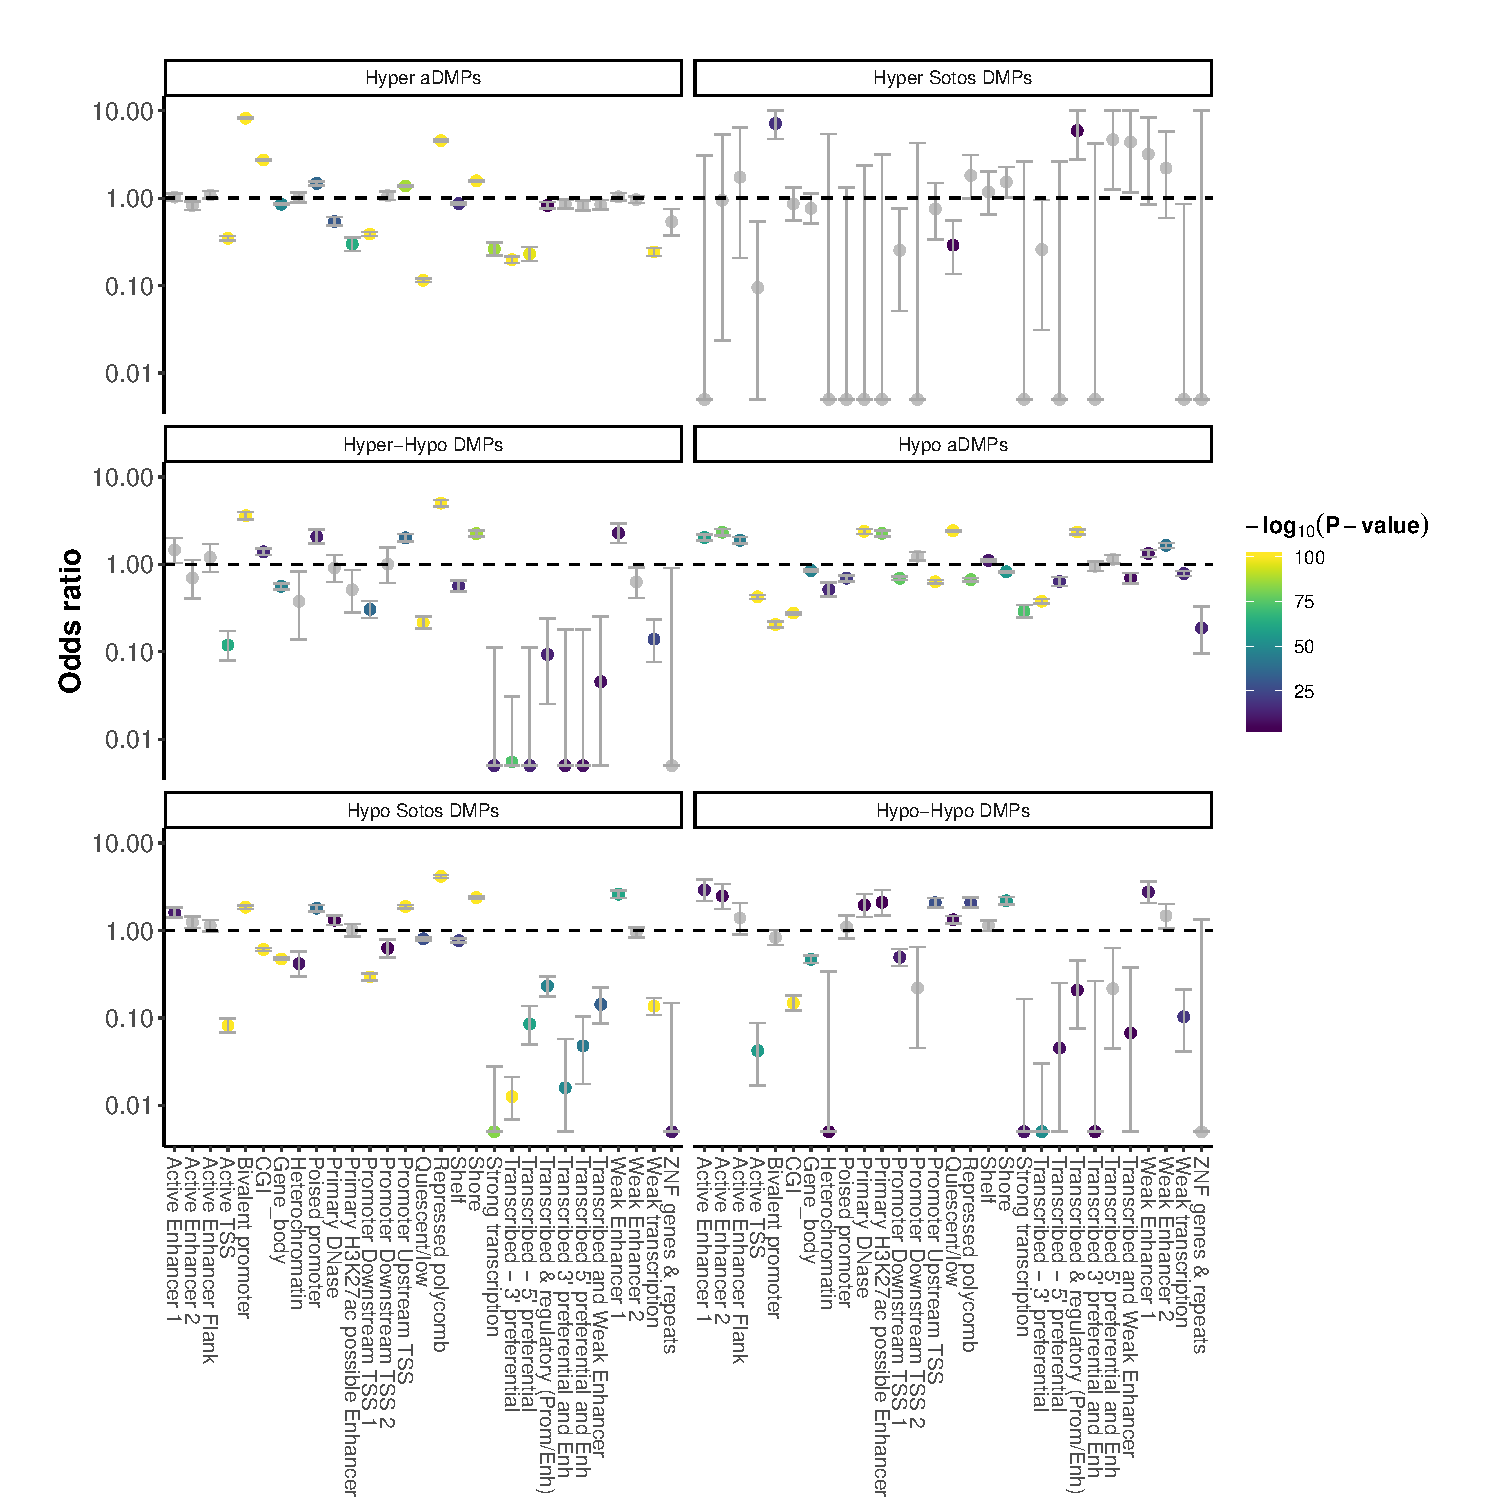
\includegraphics[width=1.1\textwidth]{SC3_Fig4}
	\vspace*{2 mm}
	\caption[Enrichment for the categorical (epi)genomic features in Sotos and ageing: genome-wide]{Enrichment for the categorical (epi)genomic features considered when comparing the different genome-wide subsets of differentially methylated positions (DMPs) in ageing and Sotos against a control (see section~\ref{s:3.7}). The y-axis represents the odds ratio (OR), the error bars show the 95\% confidence interval for the OR estimate and the colour of the points codes for $-\log_{10}(\text{p-value})$ obtained after testing for enrichment using Fisher's exact test. An OR > 1 shows that the given feature is enriched in the subset of DMPs considered, whilst an OR < 1 shows that it is found less than expected. The `Hyper-Hypo DMPs' subset results from the intersection between the hypermethylated DMPs in ageing and the hypomethylated DMPs in Sotos. The `Hypo-Hypo DMPs' subset results from the intersection between the hypomethylated DMPs in ageing and Sotos. In grey: features that did not reach significance using a significance level of $\alpha = 0.01$ after Bonferroni correction.}
	\label{fig:sc3_fig4}
\end{figure}

\begin{figure}[htbp!] 
	\centering    
	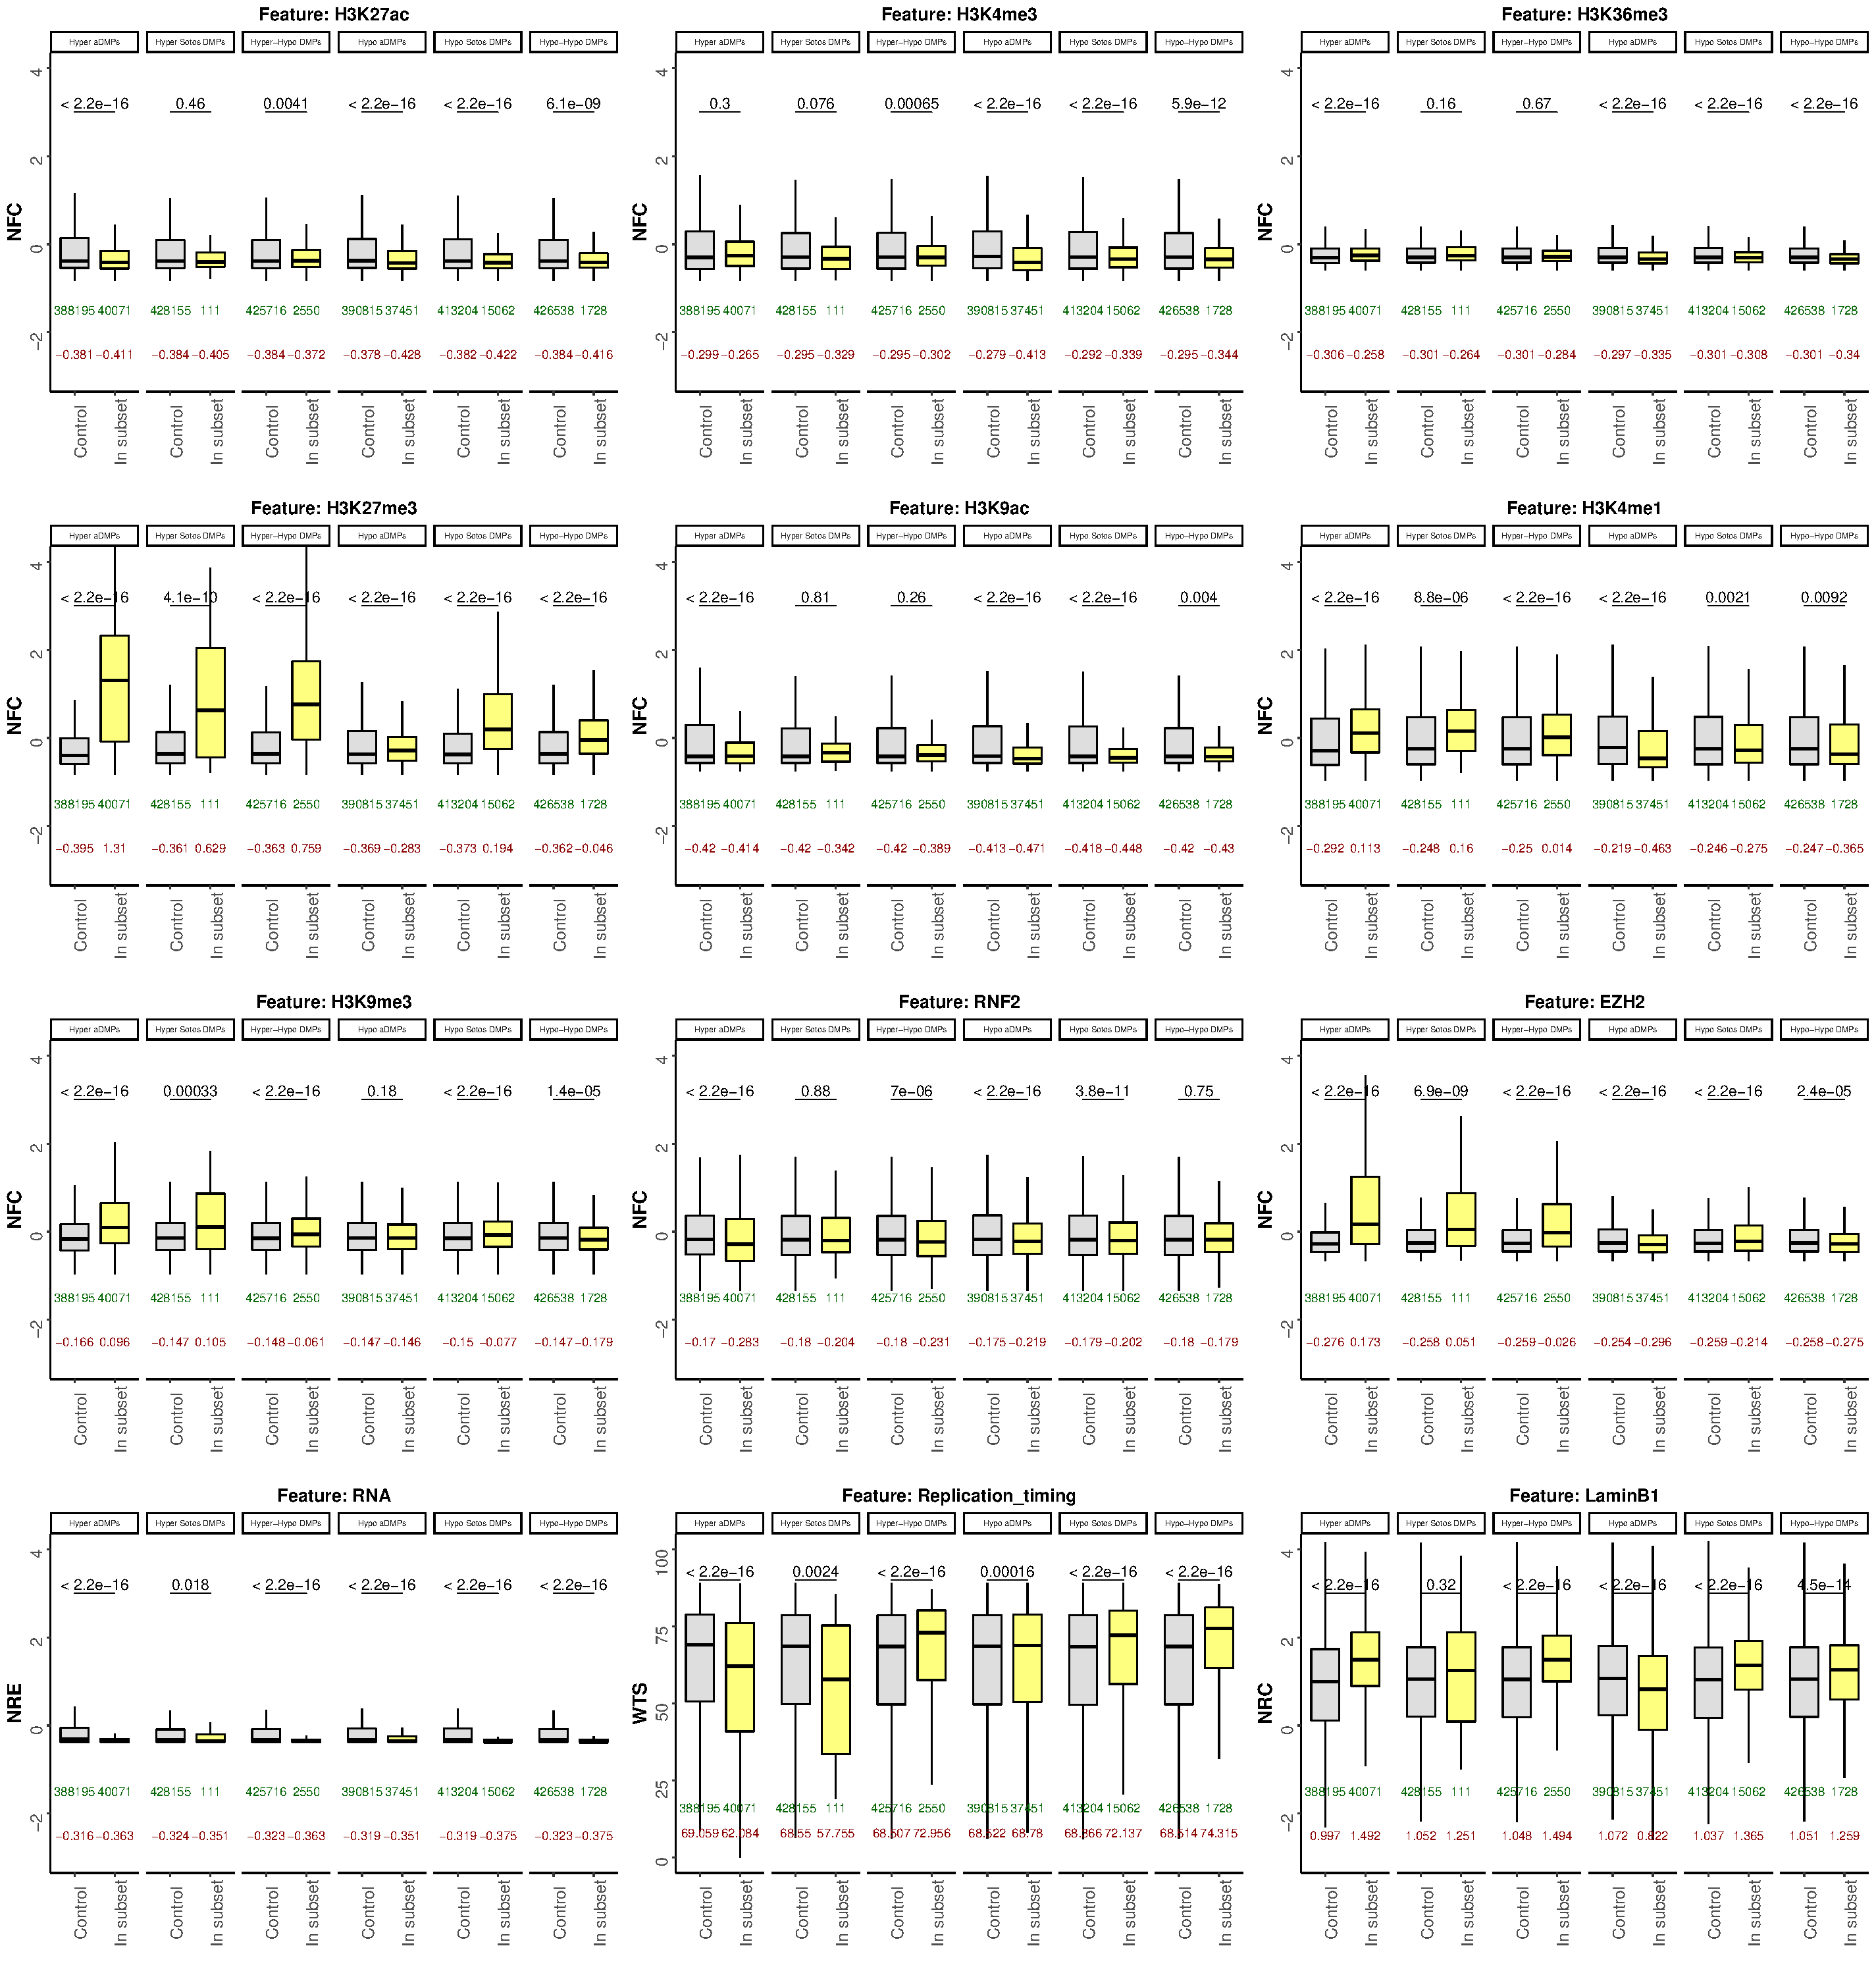
\includegraphics[width=1\textwidth]{SC3_Fig5}
	\caption[Distributions of scores for the continuous (epi)genomic features in Sotos and ageing: genome-wide]{Boxplots showing the distributions of scores for the continuous (epi)genomic features considered when comparing the different genome-wide subsets of differentially methylated positions (DMPs) in ageing and Sotos against a control (see section~\ref{s:3.7}). The p-values (two-sided Wilcoxon's test, before multiple testing correction) are shown above the boxplots. The number of DMPs belonging to each subset (in green) and the median value of the feature score (in dark red) are shown below the boxplots. \acrshort{NFC}: `normalised fold change'; \acrshort{NRE}: `normalised RNA expression'; \acrshort{WTS}: `wavelet-transformed signals'; \acrshort{NRC}: `normalised read counts'.}
	\label{fig:sc3_fig5}
\end{figure}

\begin{figure}[htbp!] 
	\centering    
	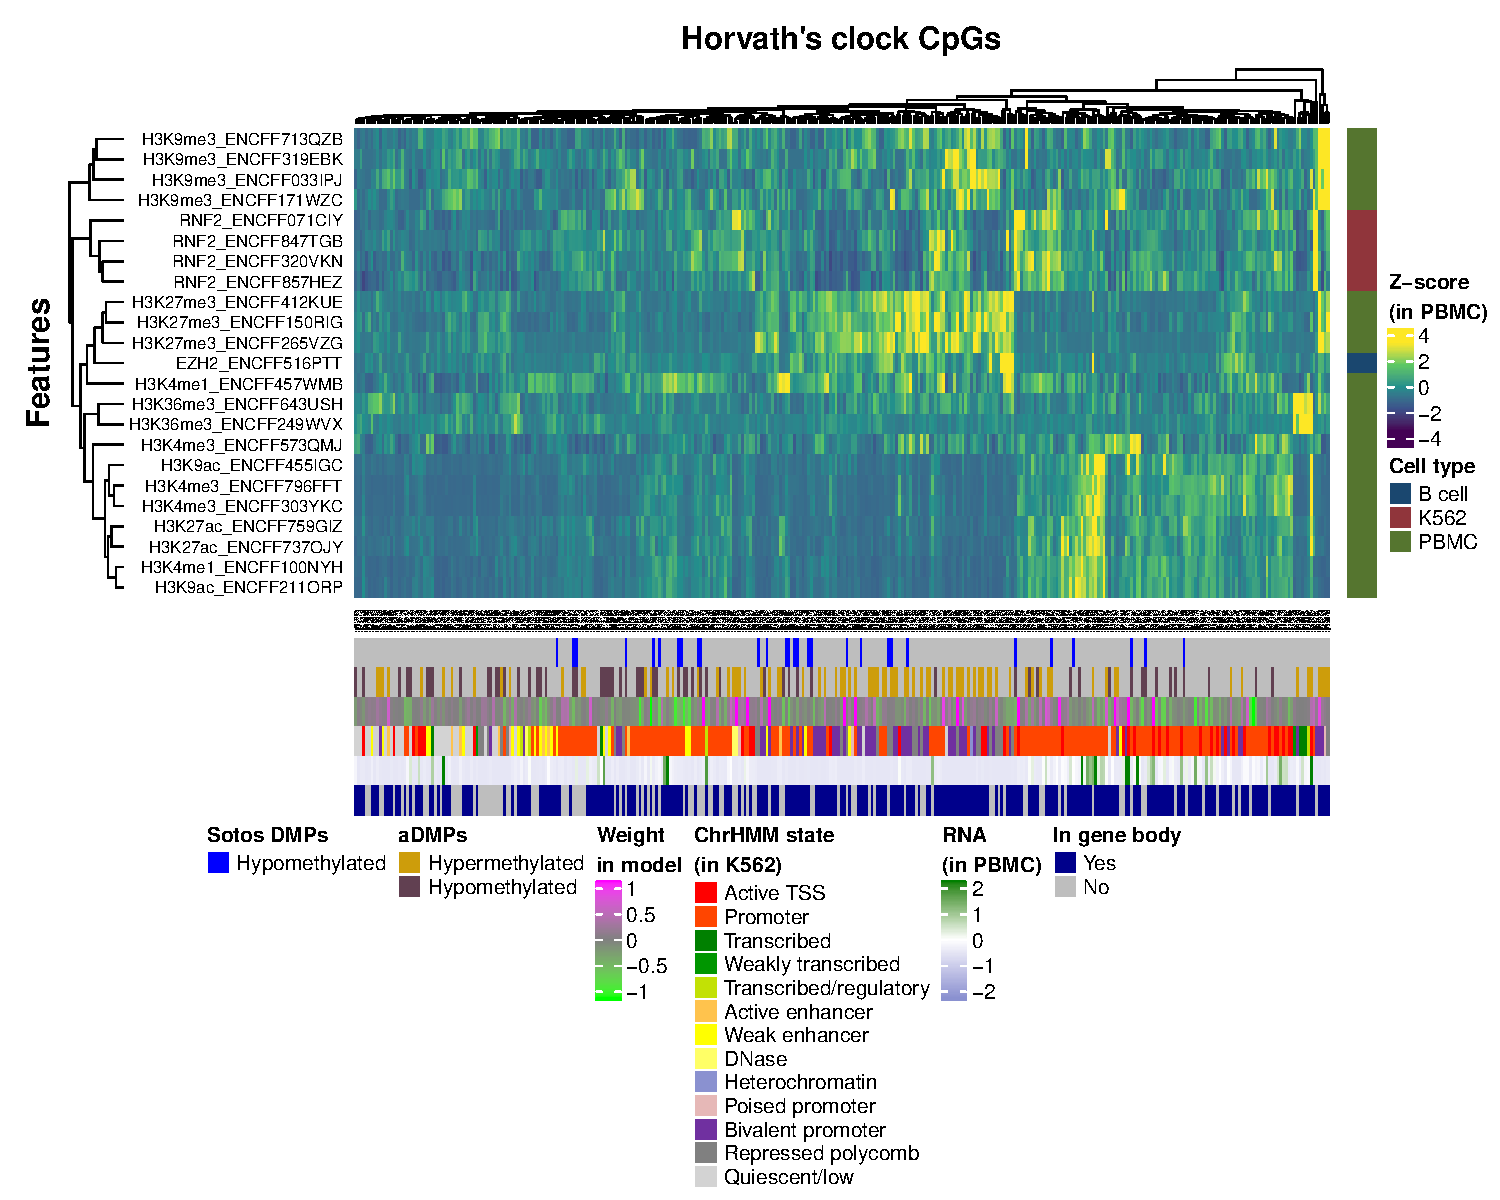
\includegraphics[width=1\textwidth]{SC3_Fig6}
	\vspace*{1 mm}
	\caption[Scores for the continuous (epi)genomic features in the Horvath's epigenetic clock CpGs]{Heatmap displaying the scores for the different continuous (epi)genomic features (rows) in each one of the 353 Horvath's epigenetic clock CpGs (columns). The names of the features include the ENCODE ID (see Fig.~\ref{fig:sc3_fig11}). Hierarchical clustering was performed in both rows and columns. RNA refers to the `normalised RNA expression' (NRE). aDMPs: differentially methylated positions during ageing. PBMC: peripheral blood mononuclear cells.}
	\label{fig:sc3_fig6}
\end{figure}

\begin{figure}[htbp!] 
	\centering    
	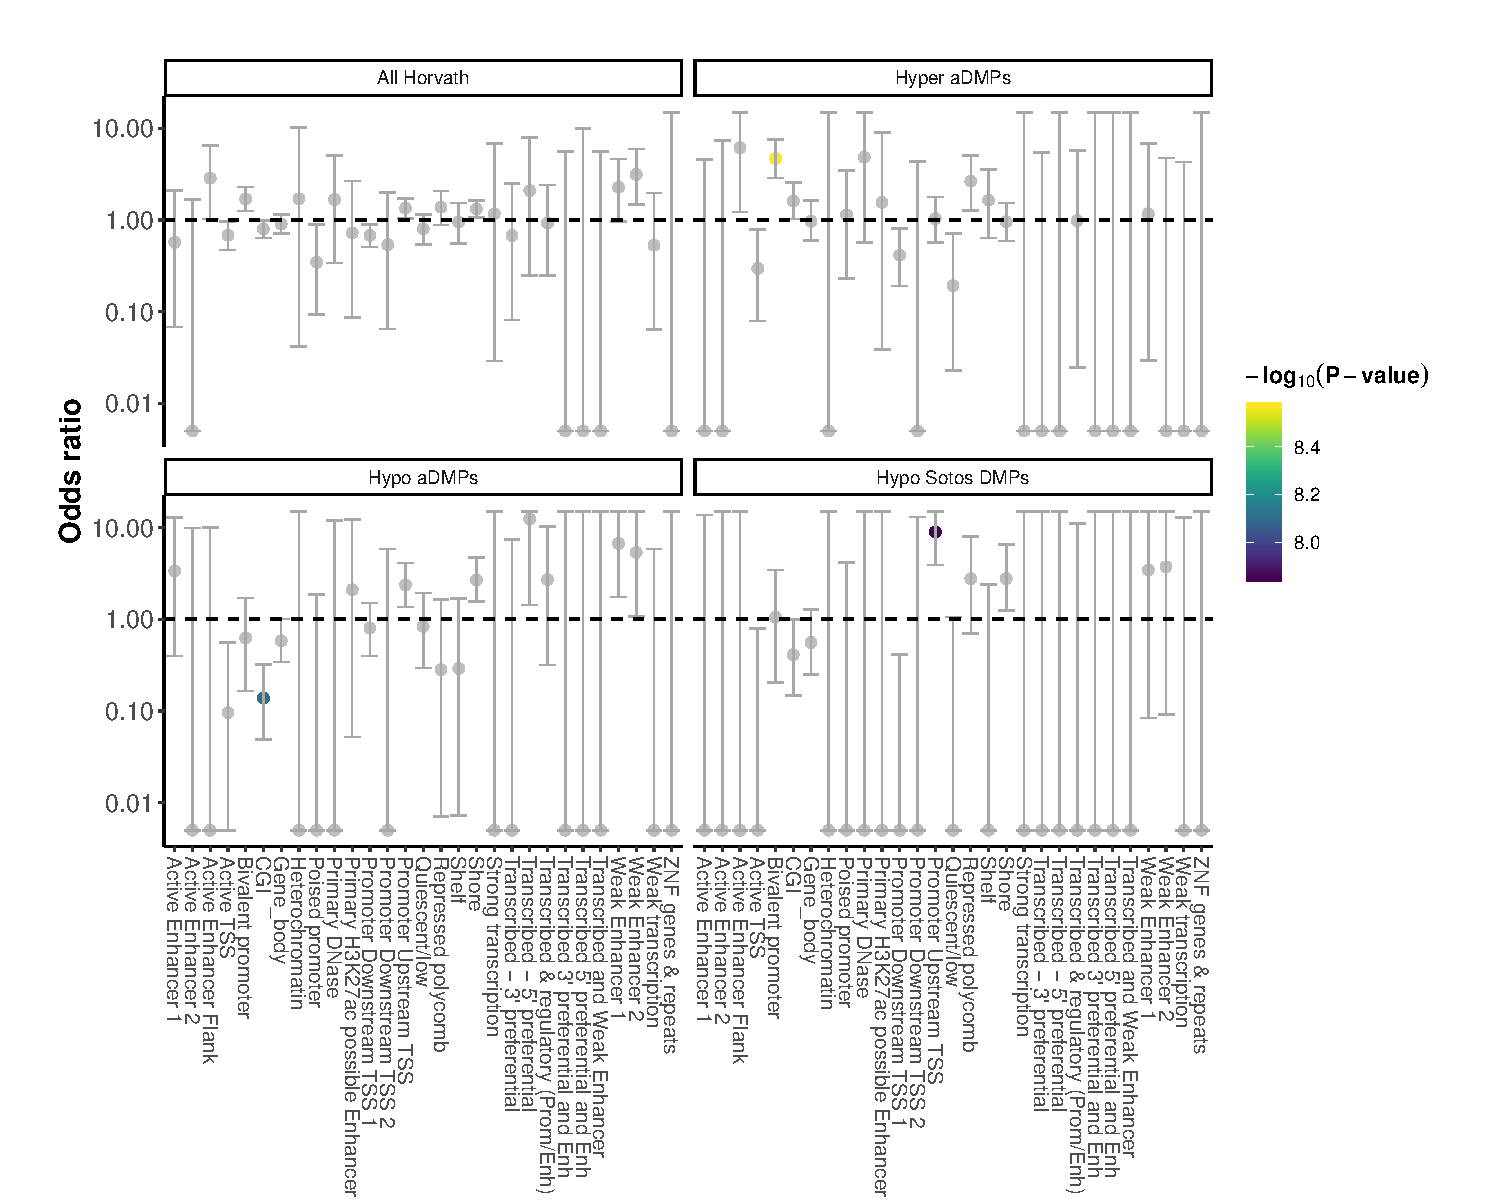
\includegraphics[width=1\textwidth]{SC3_Fig7}
	\caption[Enrichment for the categorical (epi)genomic features in Sotos and ageing: Horvath's epigenetic clock]{As in Fig.~\ref{fig:sc3_fig4}., but focused on the 353 Horvath's epigenetic clock CpG sites.}
	\label{fig:sc3_fig7}
\end{figure}

\begin{figure}[htbp!] 
	\centering    
	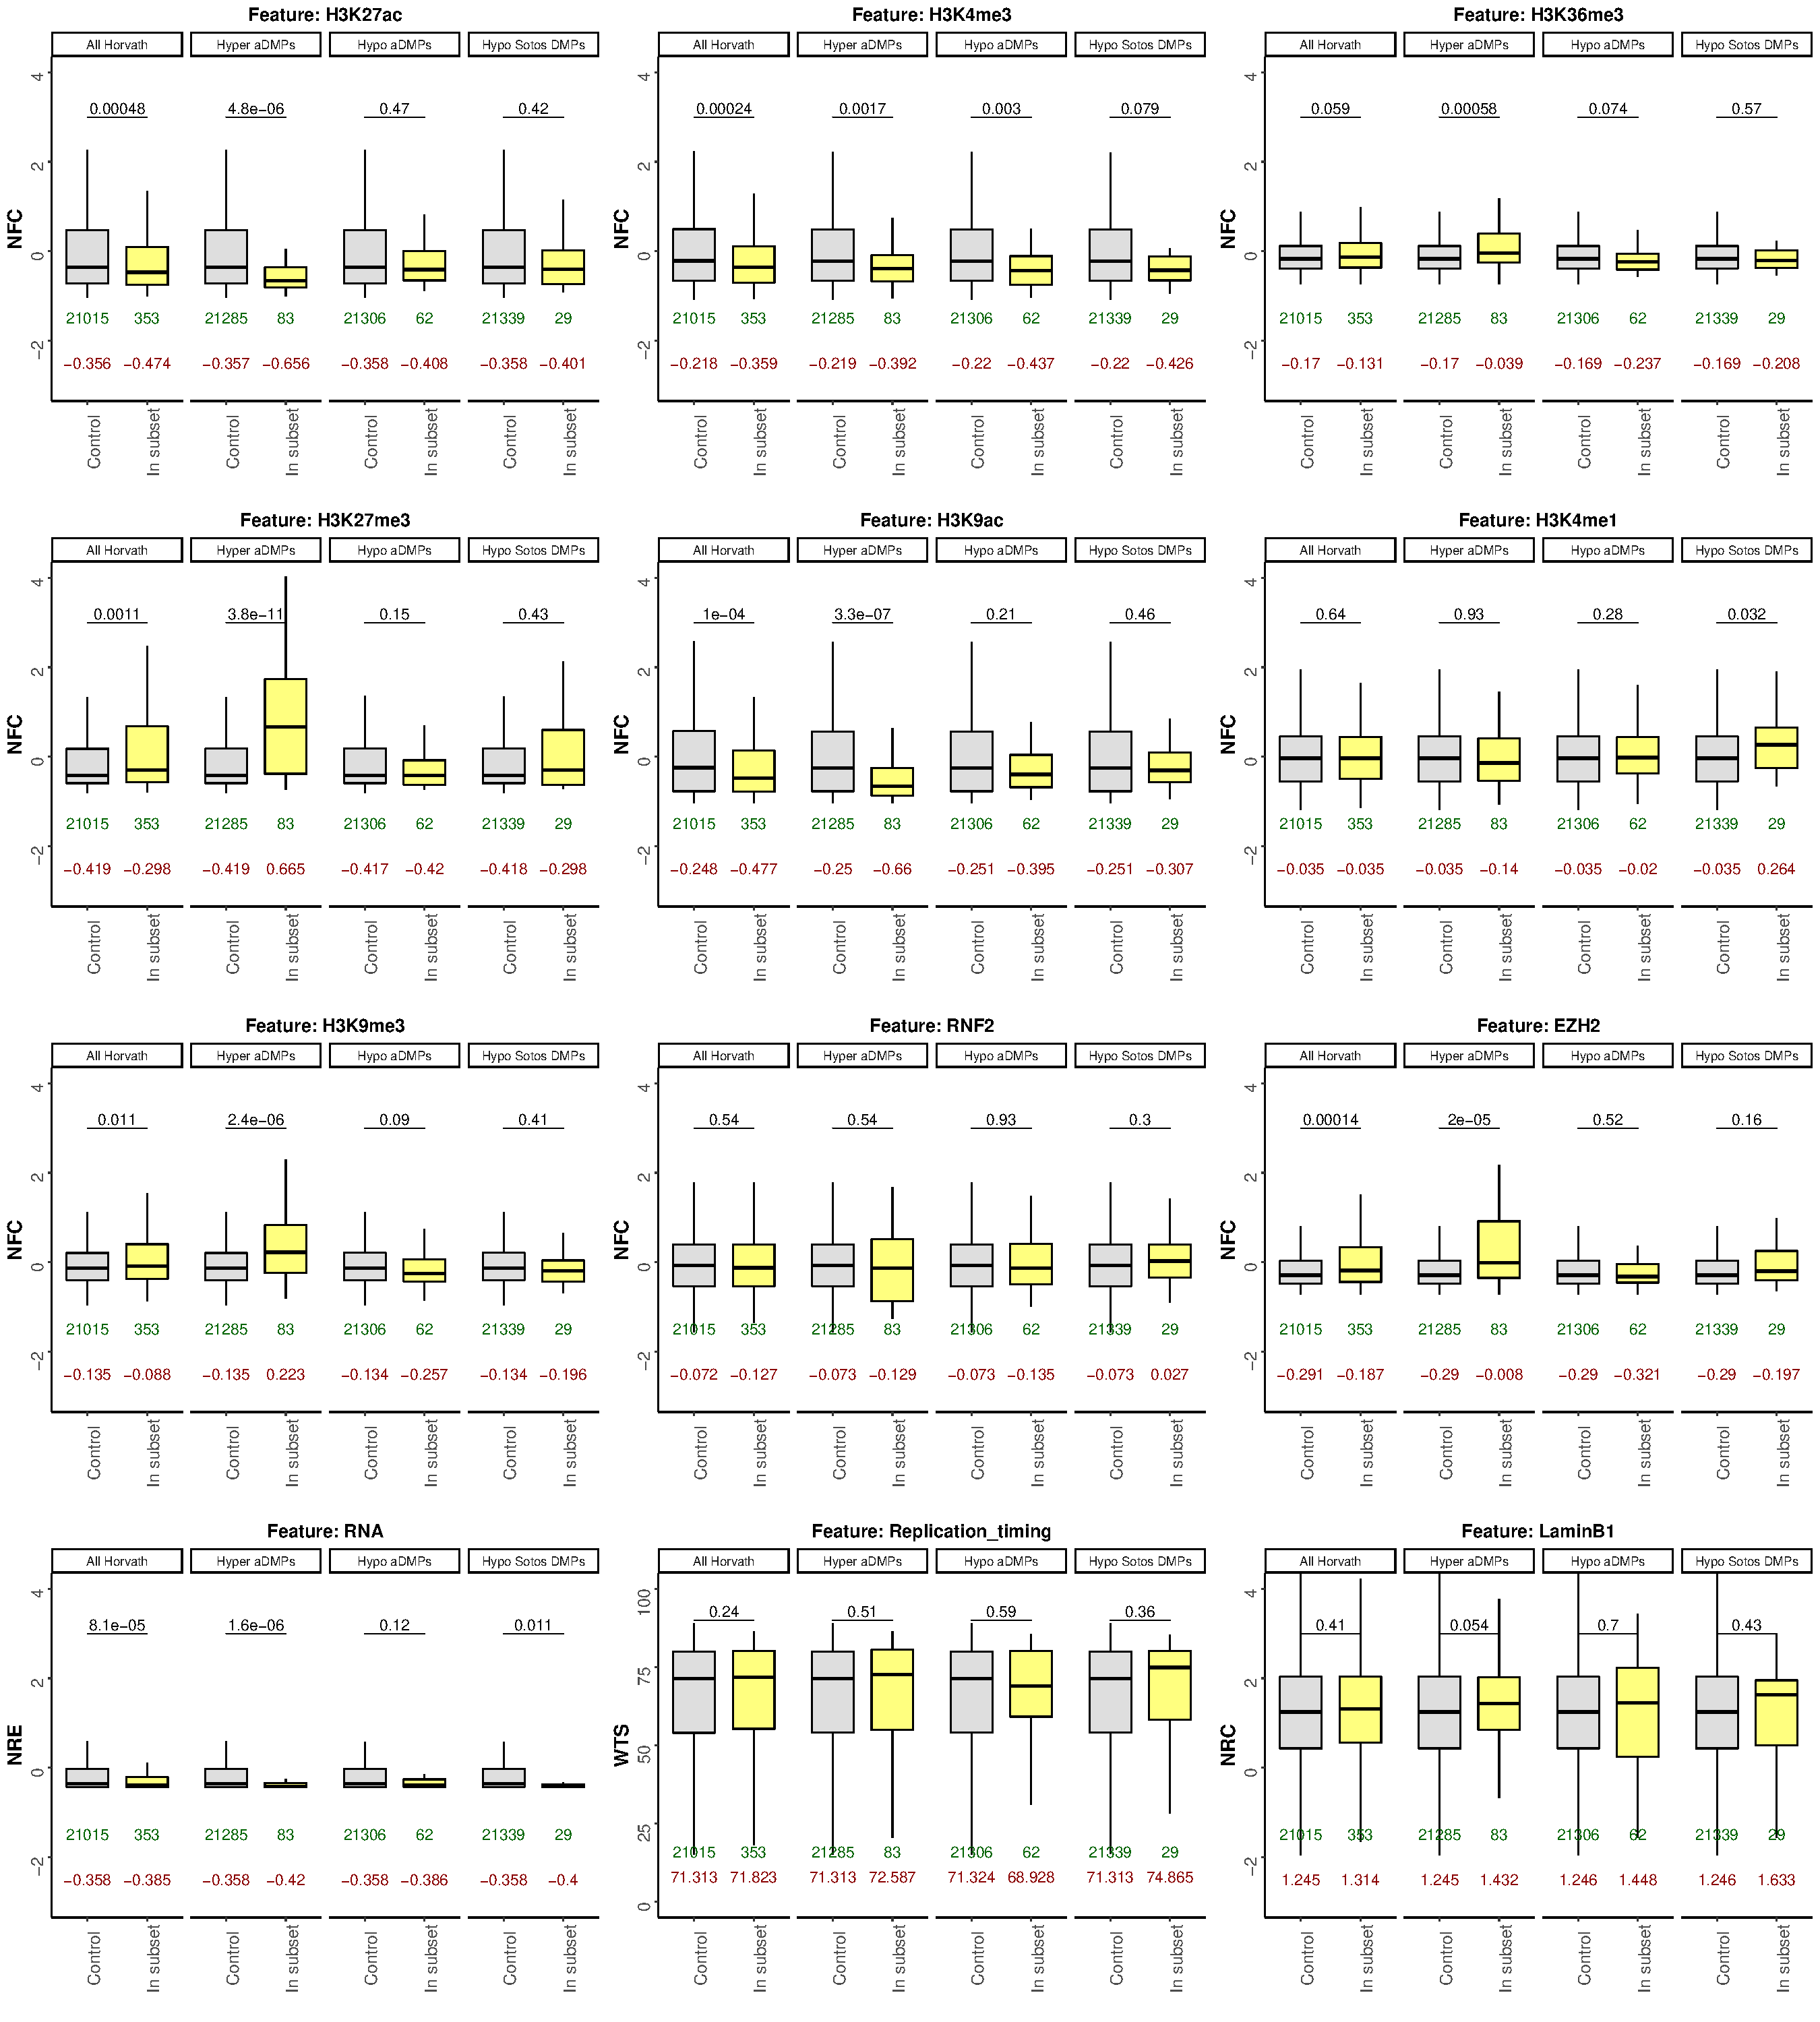
\includegraphics[width=1\textwidth]{SC3_Fig8}
	\caption[Distributions of scores for the continuous (epi)genomic features in Sotos and ageing: Horvath's epigenetic clock]{As in Fig.~\ref{fig:sc3_fig5}., but focused on the 353 Horvath's epigenetic clock CpG sites.}
	\label{fig:sc3_fig8}
\end{figure}

\begin{figure}[htbp!] 
	\centering    
	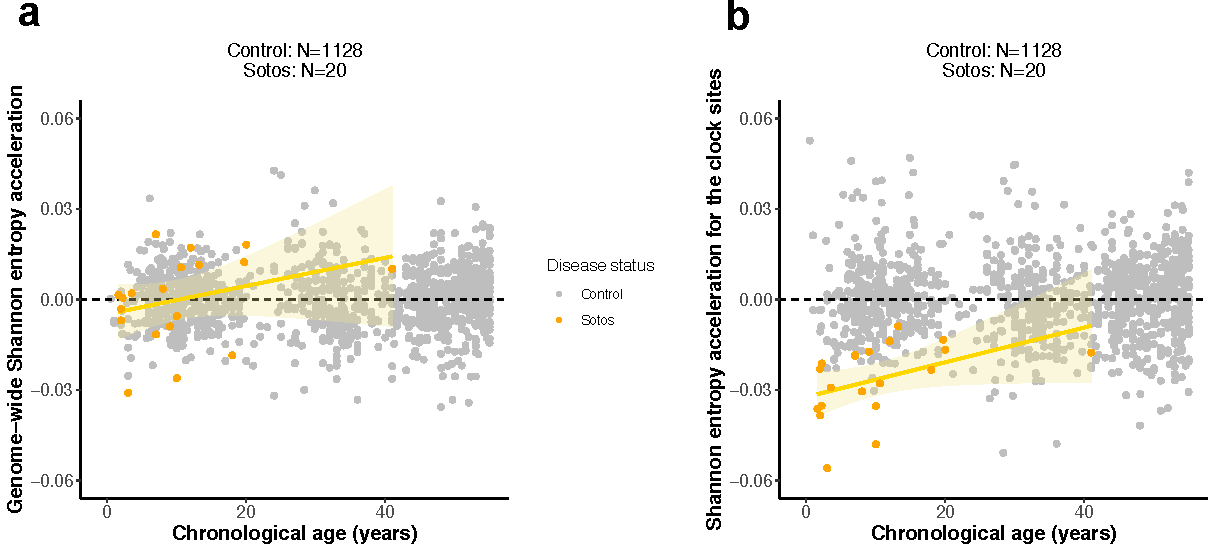
\includegraphics[width=1\textwidth]{SC3_Fig9}
	\caption[Methylation Shannon entropy acceleration]{Methylation Shannon entropy acceleration. \textbf{a.} Scatterplot showing the relationship between the genome-wide Shannon entropy acceleration (\acrshort{gSEA}) and chronological age of the samples for Sotos (orange) and healthy controls (grey). Each sample is represented by one point. The yellow line represents the linear model gSEA $\sim$ Age, with the standard error shown in the light yellow shade. \textbf{b.} As in a., but using the Shannon entropy acceleration calculated only for the 353 CpG sites in the Horvath's epigenetic clock (\acrshort{cSEA}).}
	\label{fig:sc3_fig9}
\end{figure}

\begin{figure}[htbp!] 
	\centering    
	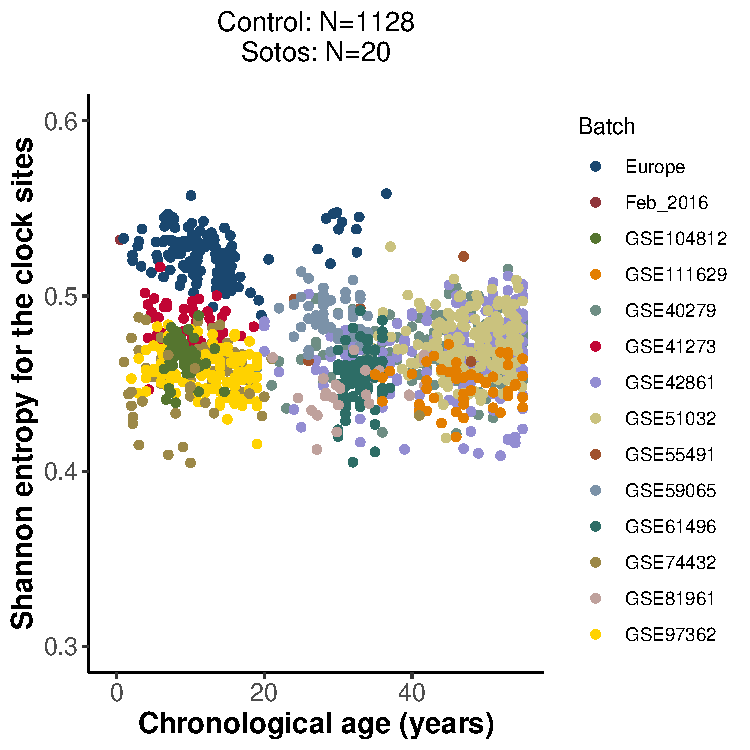
\includegraphics[width=0.5\textwidth]{SC3_Fig10}
	\caption[Batch effects in the methylation Shannon entropy for the epigenetic clock sites]{Scatterplot showing the effects of the different batches on the methylation Shannon entropy calculations for the 353 Horvath's epigenetic clock sites. Each sample is represented by one point and coloured according to the batch that they belong to. }
	\label{fig:sc3_fig10}
\end{figure}

		

\begin{figure}[htbp!] 
	\centering    
	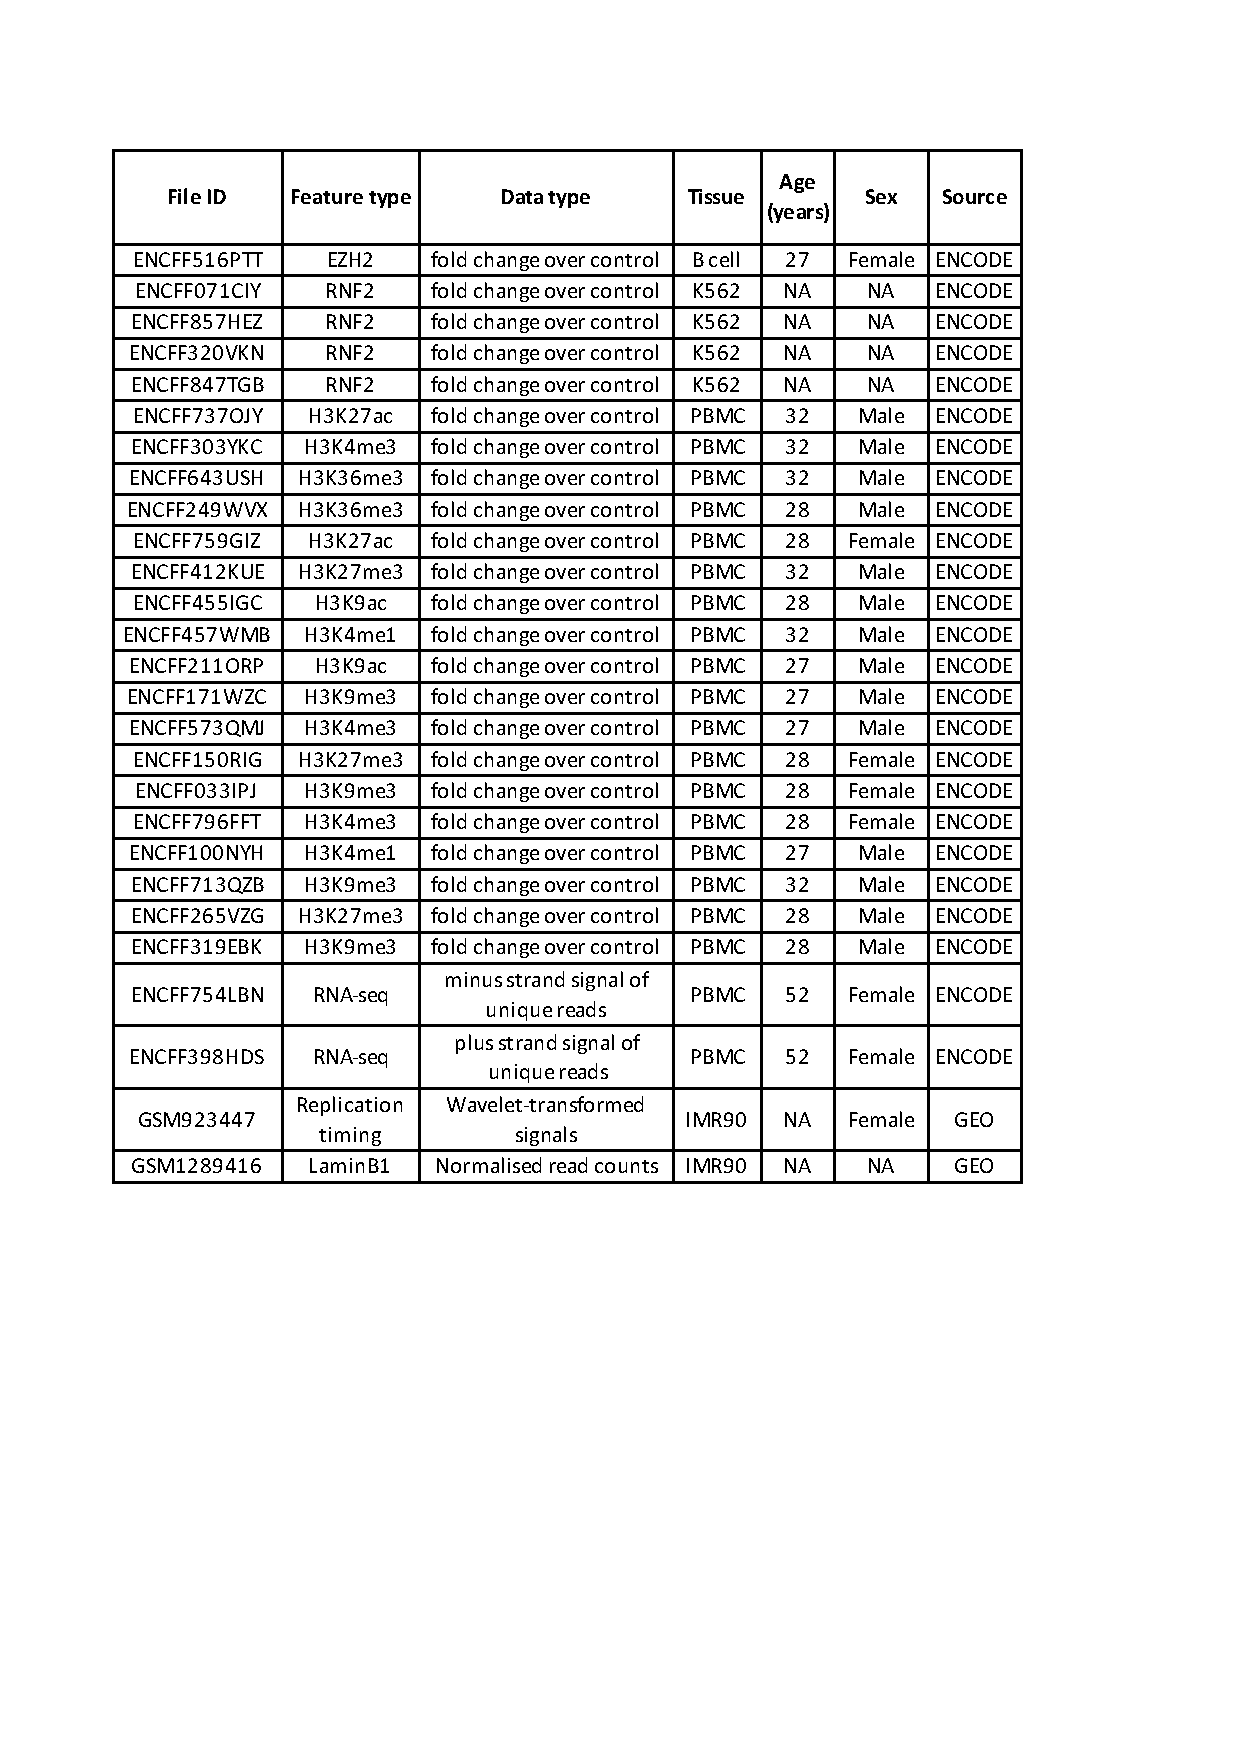
\includegraphics[width=1\textwidth]{SC3_Fig11}
	\caption[Information for the continuous (epi)genomic features]{Information (including the source) about the continuous (epi)genomic features (\acrshort{ChIP-seq} and \acrshort{RNA-seq} data) that were included in my analysis to annotate the different sets of CpG sites. All the data were mapped to the \textit{\acrshort{hg19}} assembly of the human genome. \acrshort{PBMC}: peripheral blood mononuclear cells.}
	\label{fig:sc3_fig11}
\end{figure}

\clearpage

\renewcommand{\thesection}{S.3}   
\section{Technological aspects of epigenetic clocks}

\renewcommand\thefigure{S3.\arabic{figure}}    
\bigskip

\begin{figure}[htbp!] 
	\centering    
	\setcounter{figure}{0}
	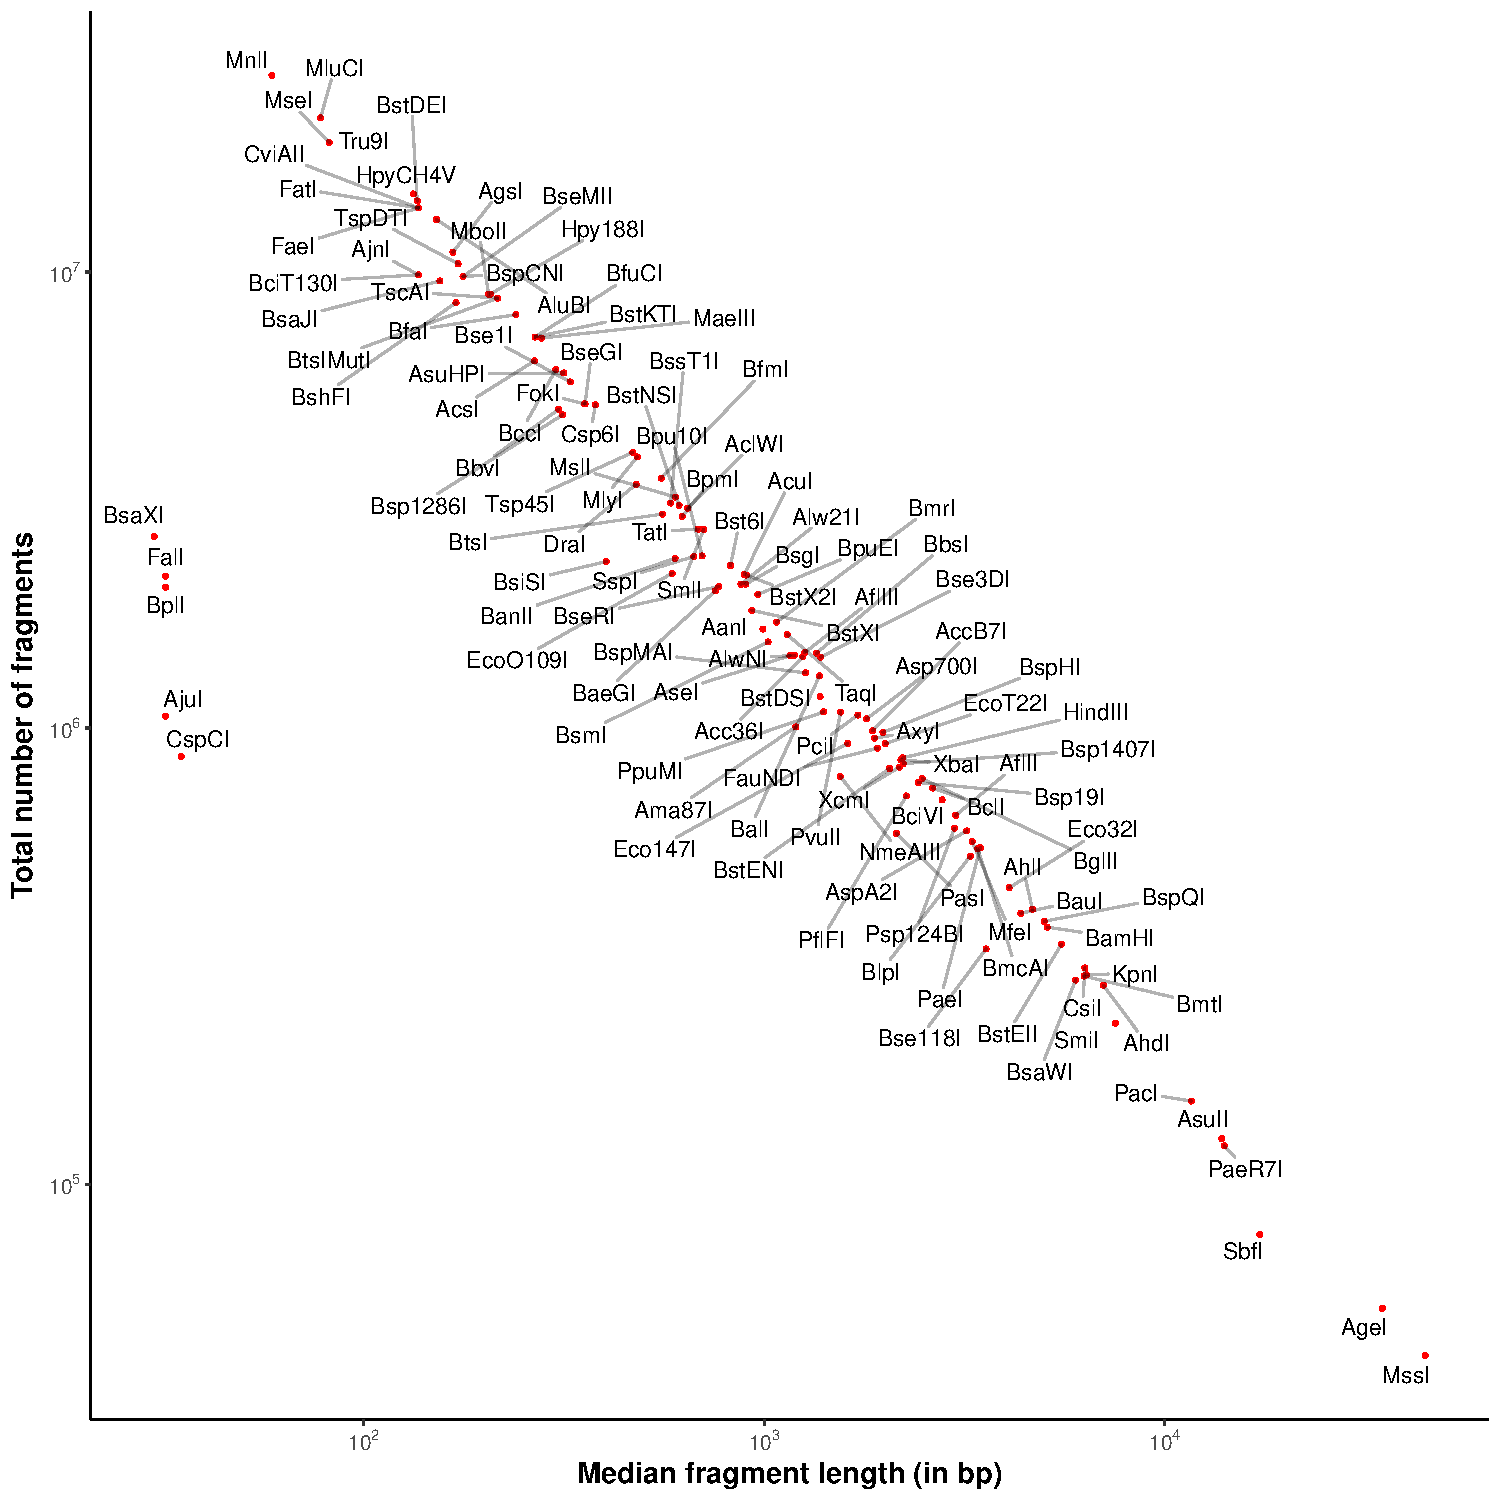
\includegraphics[width=0.7\textwidth]{SC4_Fig1}
	\caption[Scatterplot of fragment length distributions for the isoschizomer families]{Scatterplot which summarises the fragment length distributions for the same isoschizomer families portrayed in Fig~\ref{fig:c4_fig2}a. The red dots represent the actual values of median fragment length and total number of fragments for each family. The black lines assign each name label to the correspondent red point for visualization purposes.}
	\label{fig:sc4_fig1}
\end{figure}

\begin{figure}[htbp!] 
	\centering    
	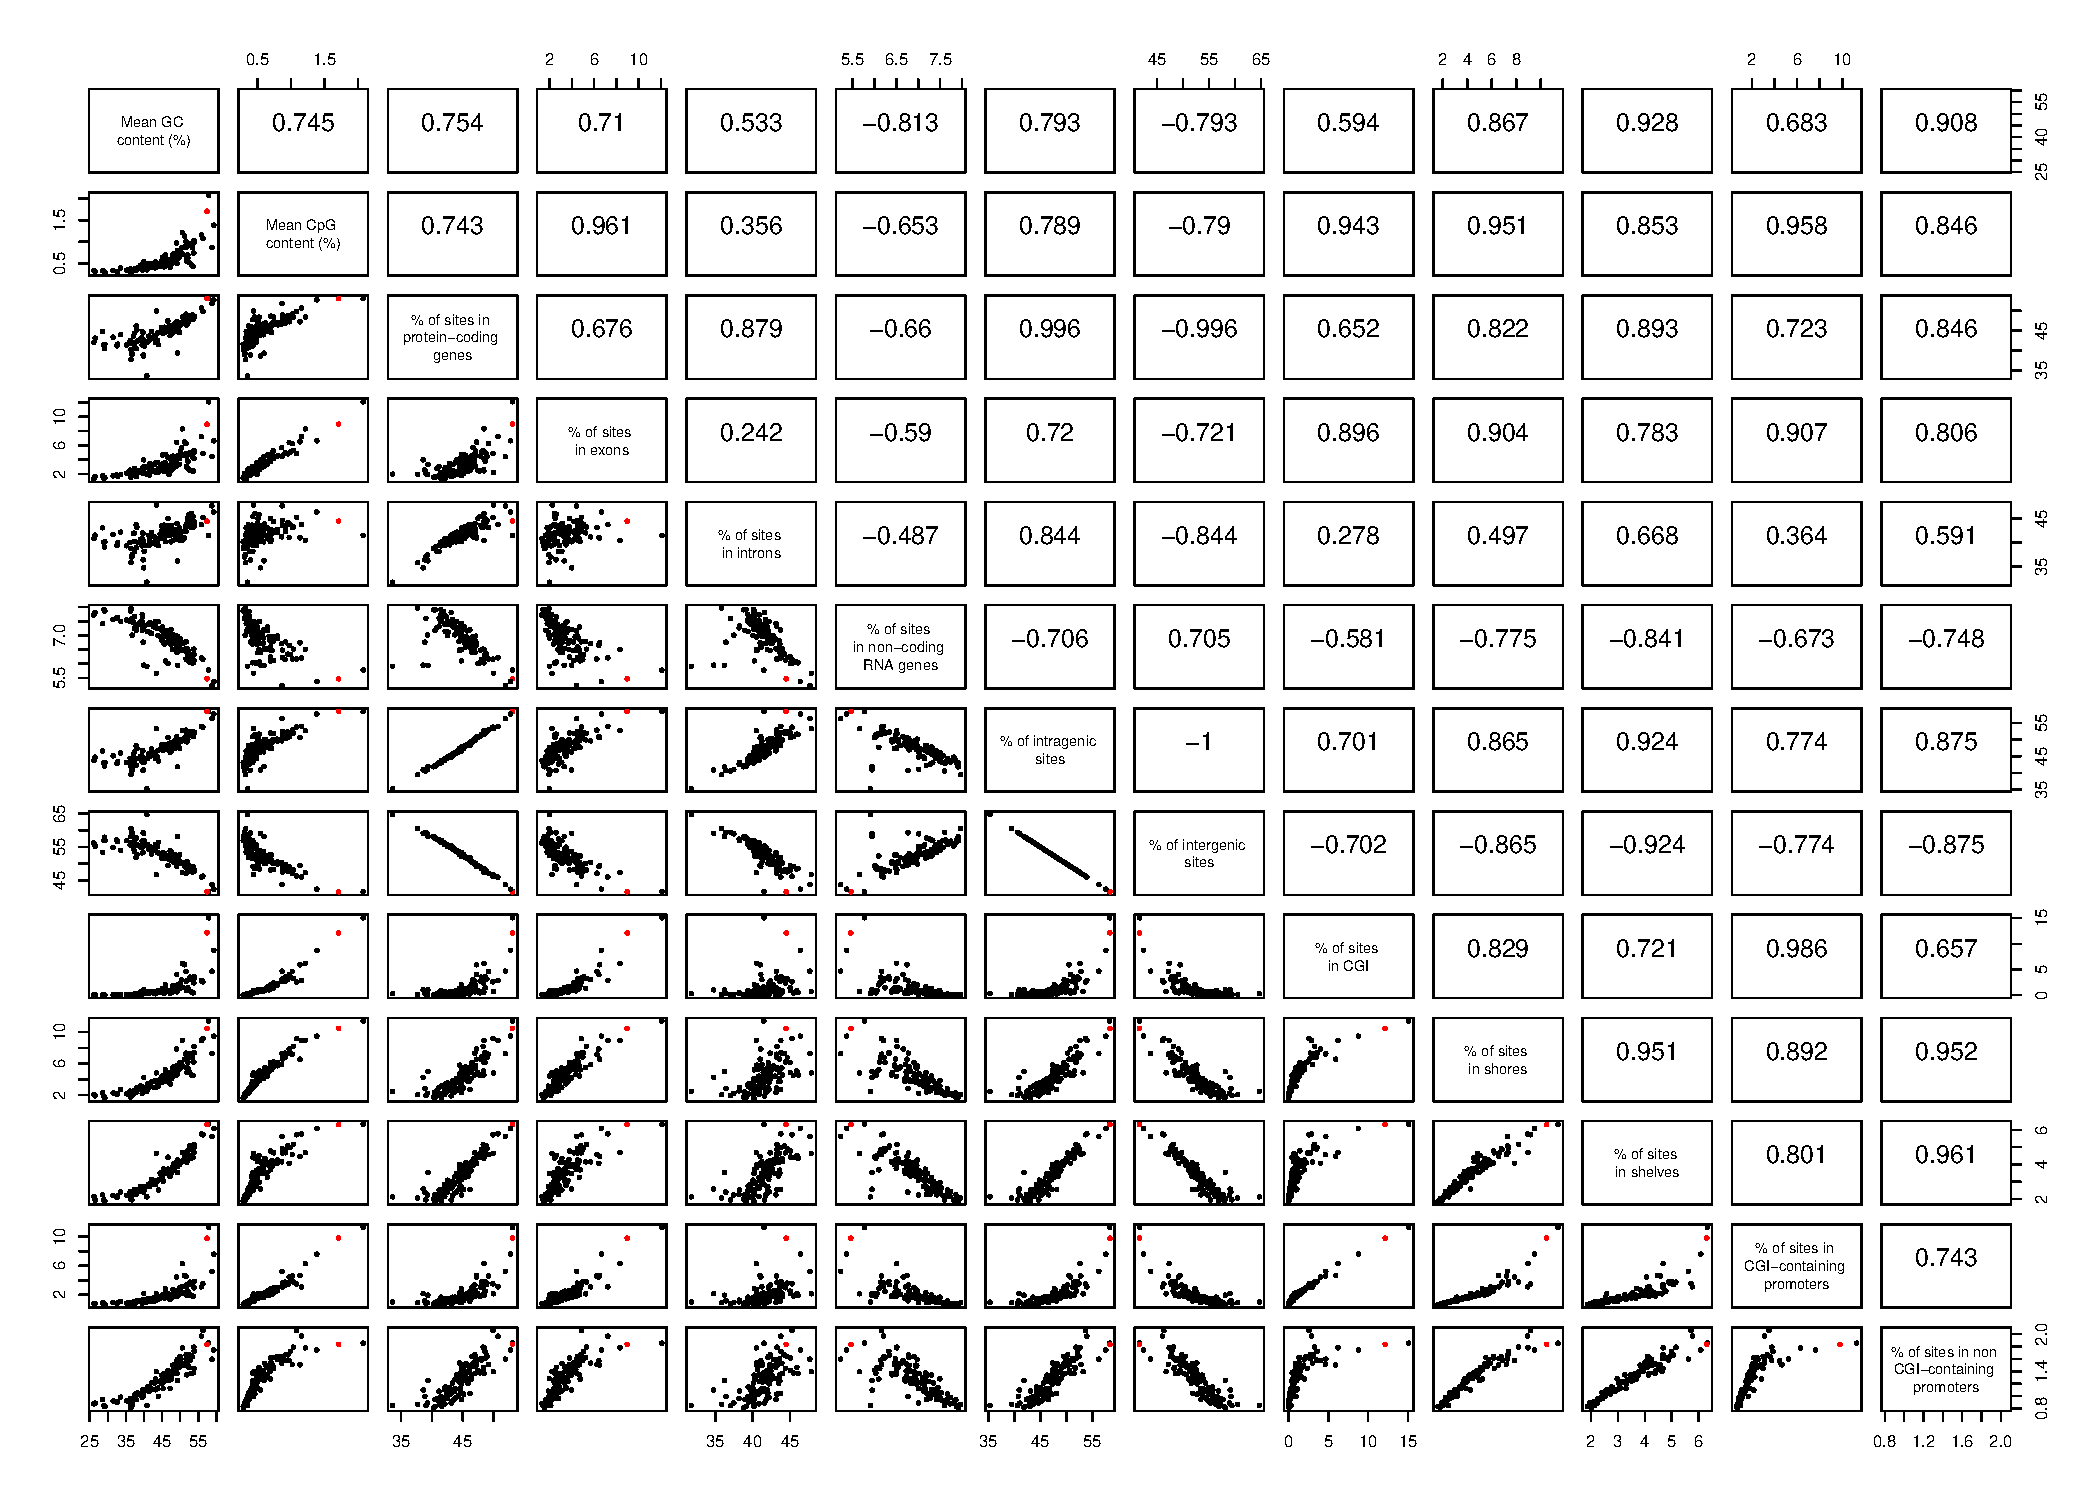
\includegraphics[width=1\textwidth]{SC4_Fig2}
	\caption[Genomic features that overlap with restriction enzyme cleavage sites]{Matrix of scatterplots showing the percentages of cleavage sites from different restriction enzymes that overlap with several genomic features (listed on the diagonal) in the human genome (hg38). The red dot in each scatterplot represents the values for MspI. The numbers above the diagonal are the Pearson correlation coefficients between all the possible pairs of genomic features.}
	\label{fig:sc4_fig2}
\end{figure}

\begin{figure}[htbp!] 
	\centering    
	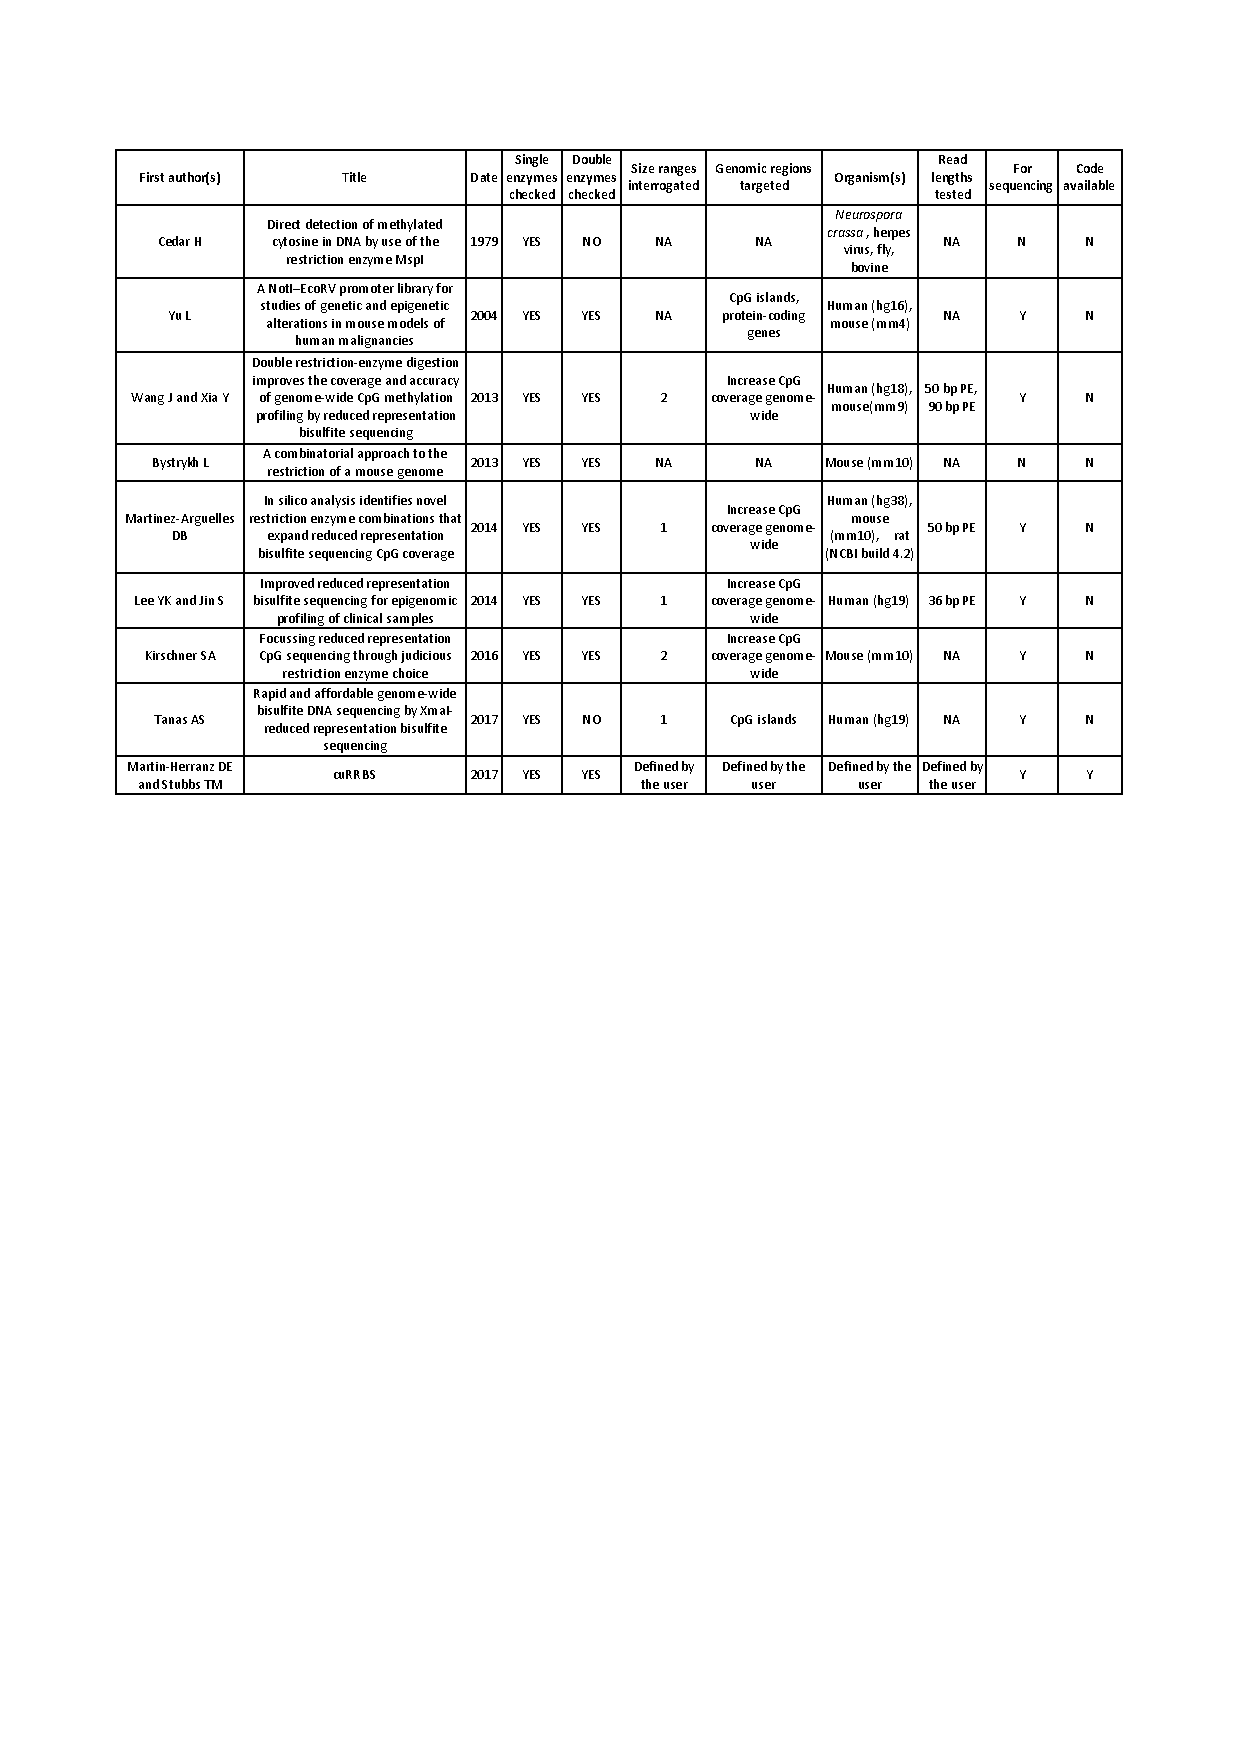
\includegraphics[width=1.0\textwidth]{SC4_Fig3}
	\caption[Comparison of studies using restriction enzymes for genomic enrichment]{Table showing the comparison of different studies that have attempted to use restriction enzymes to target different regions in the genome.}
	\label{fig:sc4_fig3}
\end{figure}

\begin{figure}[htbp!] 
	\centering    
	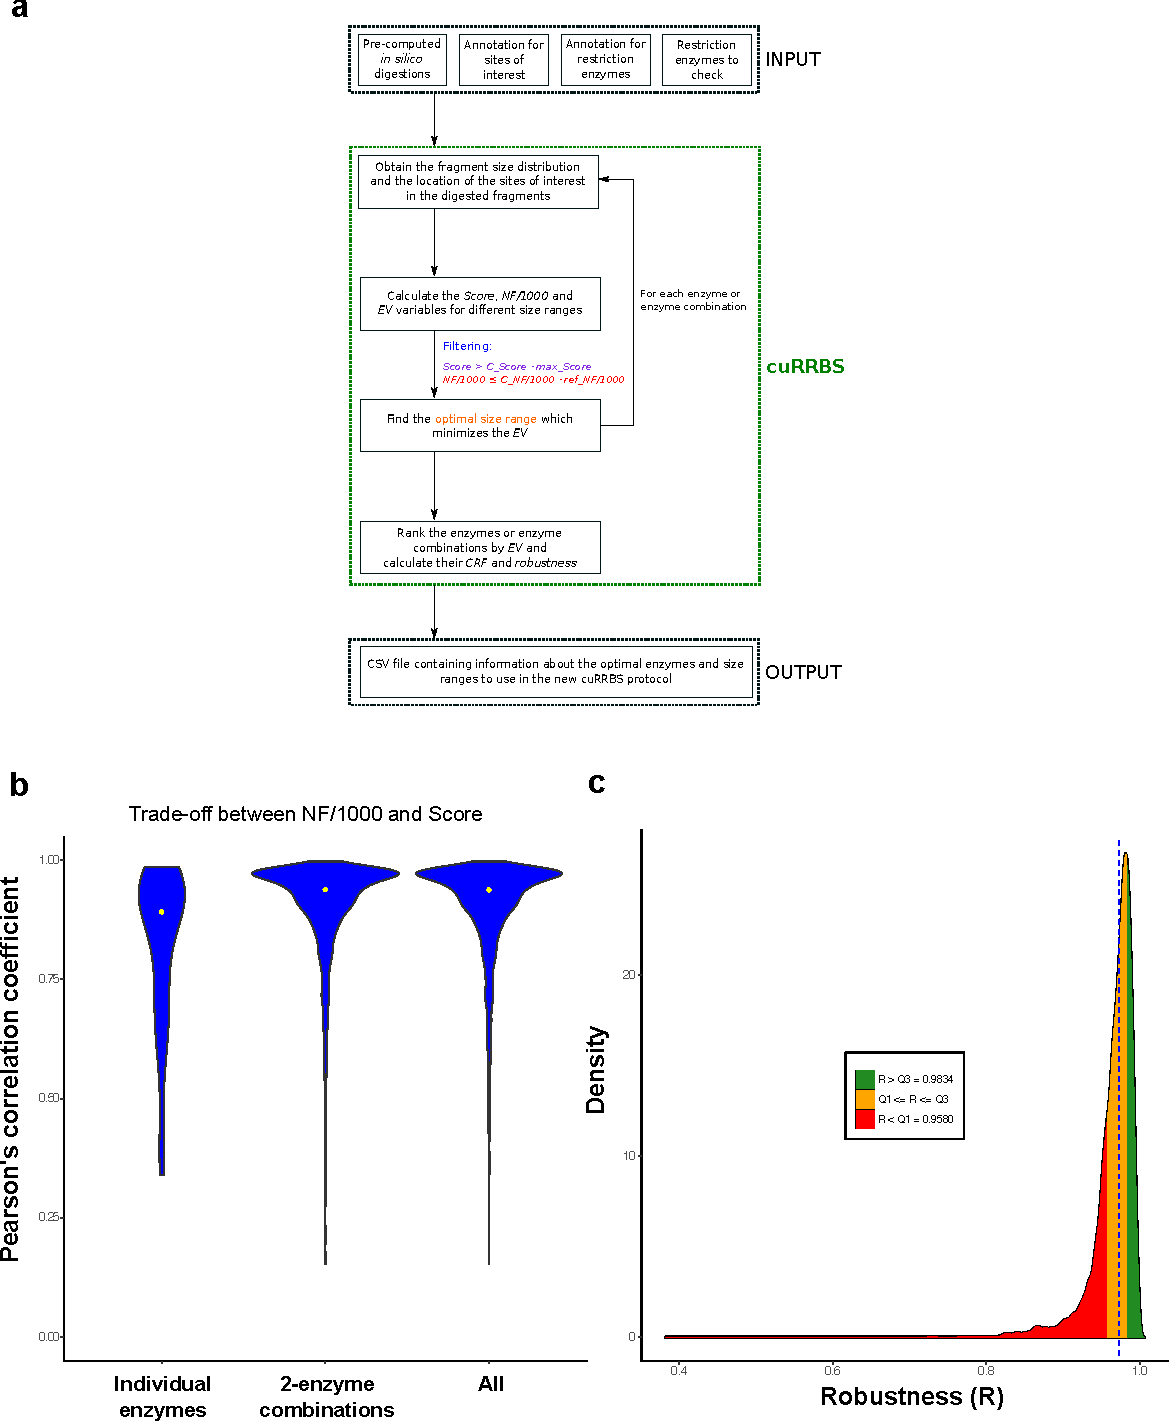
\includegraphics[width=1.0\textwidth]{SC4_Fig4}
	\vspace*{1mm}
	\caption[Additional insights into cuRRBS]{Additional insights into cuRRBS. \textbf{a.} Detailed flowchart showing the input, main steps in cuRRBS and the output of the software. \textbf{b.} Violin plots showing the distribution of Pearson's correlation coefficients between the number of fragments (\textit{NF}) and the \textit{Score} for all the different enzymes tested with cuRRBS (single-enzyme, double-enzyme, all). In this example we used the Horvath epigenetic clock system \cite{Horvath2013}, checking all the \textit{size ranges} between 20 and 1000 bp, with an \textit{experimental error} of 10 bp and a \textit{read length} of 75 bp. Each yellow point represents the median for the Pearson's correlation coefficients under consideration. \textbf{c.} Density plot showing the distribution of the \textit{robustness} (\textit{R}) values when assuming an \textit{experimental error} ($\delta$) of 20 bp. cuRRBS was run for all the biological systems under study (Fig.~\ref{fig:sc4_fig5}) \cite{Horvath2013,Hanna2016,Milagre2017,Kawakatsu2016,Maurano2015,LevMaor2015,Domcke2015} with the same parameters as described in `Running cuRRBS for different \textit{in silico} systems' in section~\ref{s:4.7} (all the hits that satisfied the \textit{thresholds} were reported in this case). The dashed blue line represents the median (0.9734). The different colours provide a way to judge the \textit{robustness} values: bad (in red, $R < Q_1 = 0.9580$), medium (in orange, $Q_1 \leq R \leq Q_3 = 0.9834$) and good (in green, $R > Q_3$); where $Q_1$ and $Q_3$ represent the first and the third quartiles respectively.}
	\label{fig:sc4_fig4}
\end{figure}

\begin{figure}[htbp!] 
	\centering    
	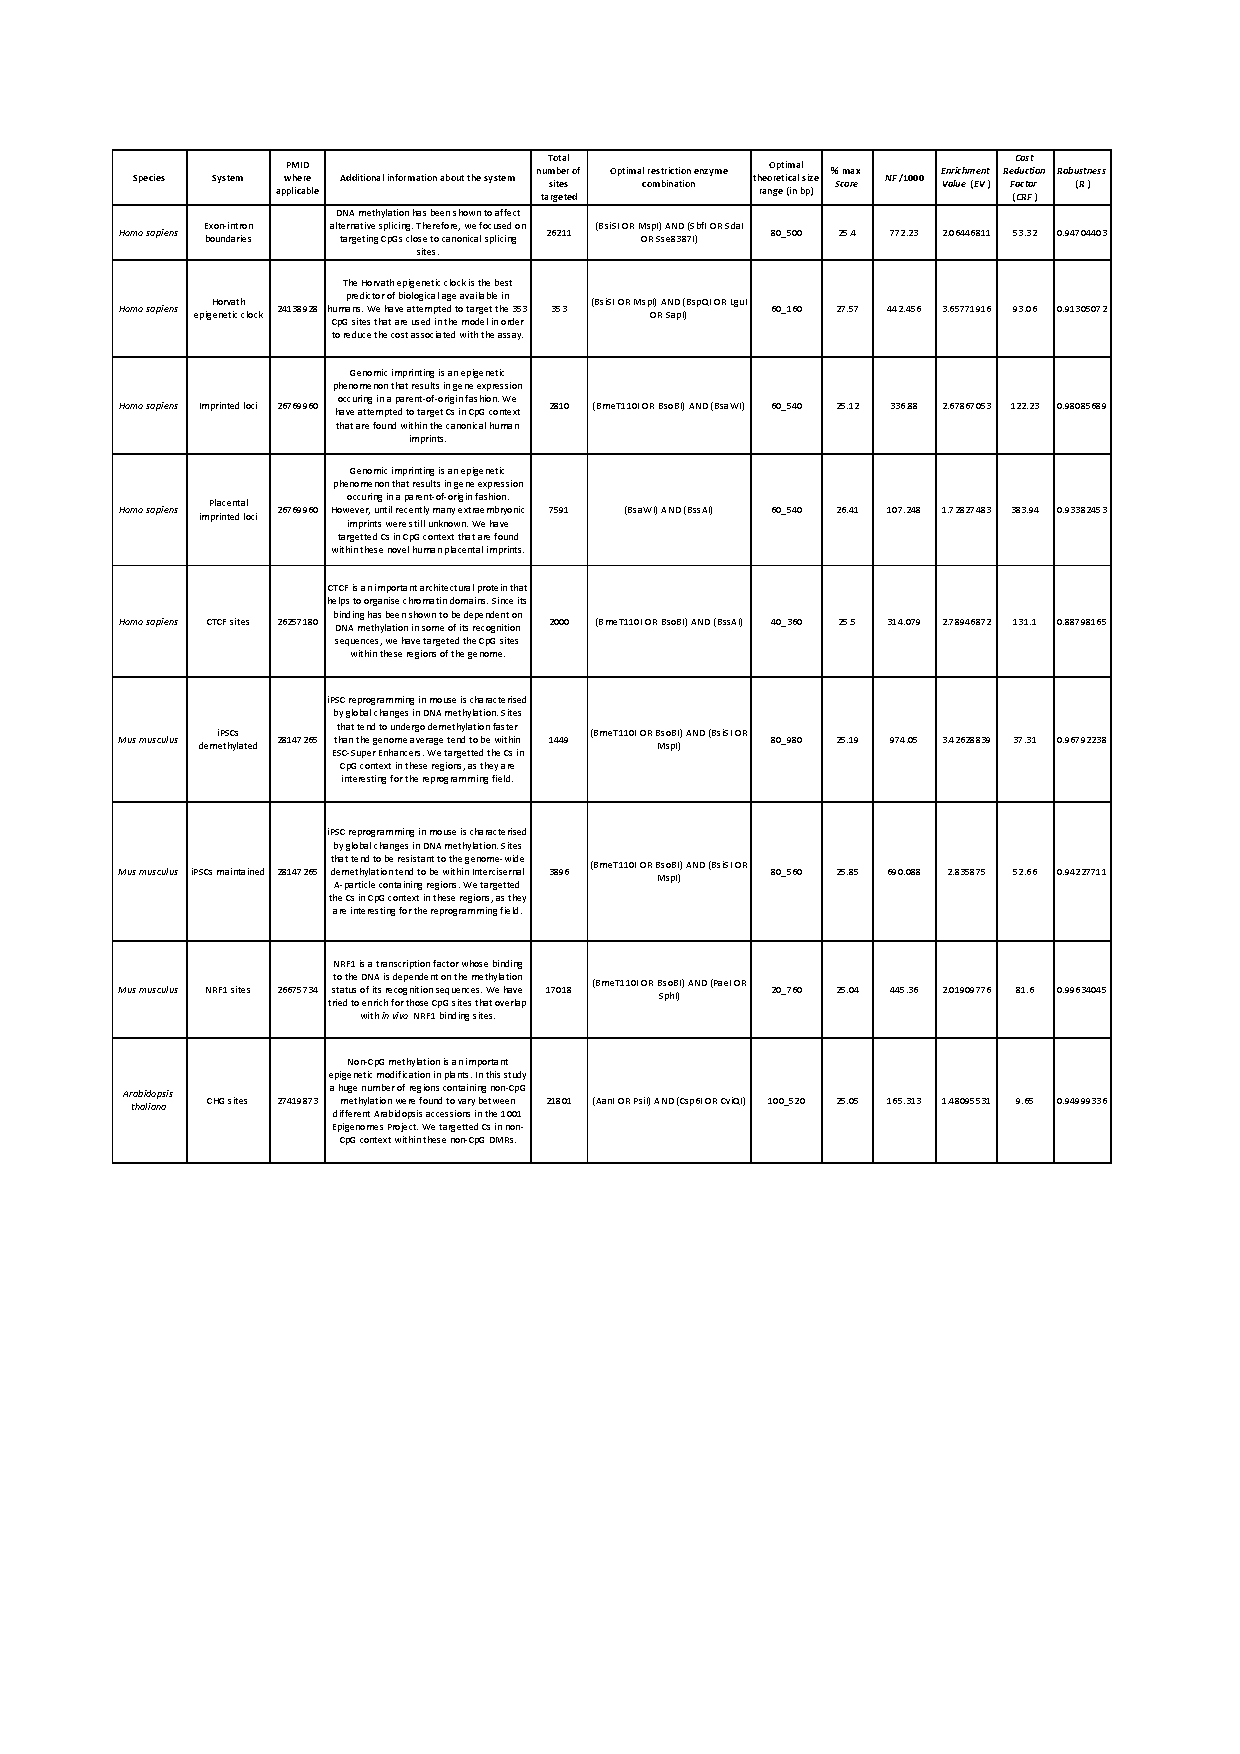
\includegraphics[width=1.0\textwidth]{SC4_Fig5}
	\caption[Additional results of running cuRRBS in different biological systems]{Table showing the information regarding the different biological systems \cite{Horvath2013,Hanna2016,Milagre2017,Kawakatsu2016,Maurano2015,LevMaor2015,Domcke2015} for which cuRRBS was run \textit{in silico}. Some variables from the top hits in cuRRBS output are also reported.}
	\label{fig:sc4_fig5}
\end{figure}

\begin{figure}[htbp!] 
	\centering    
	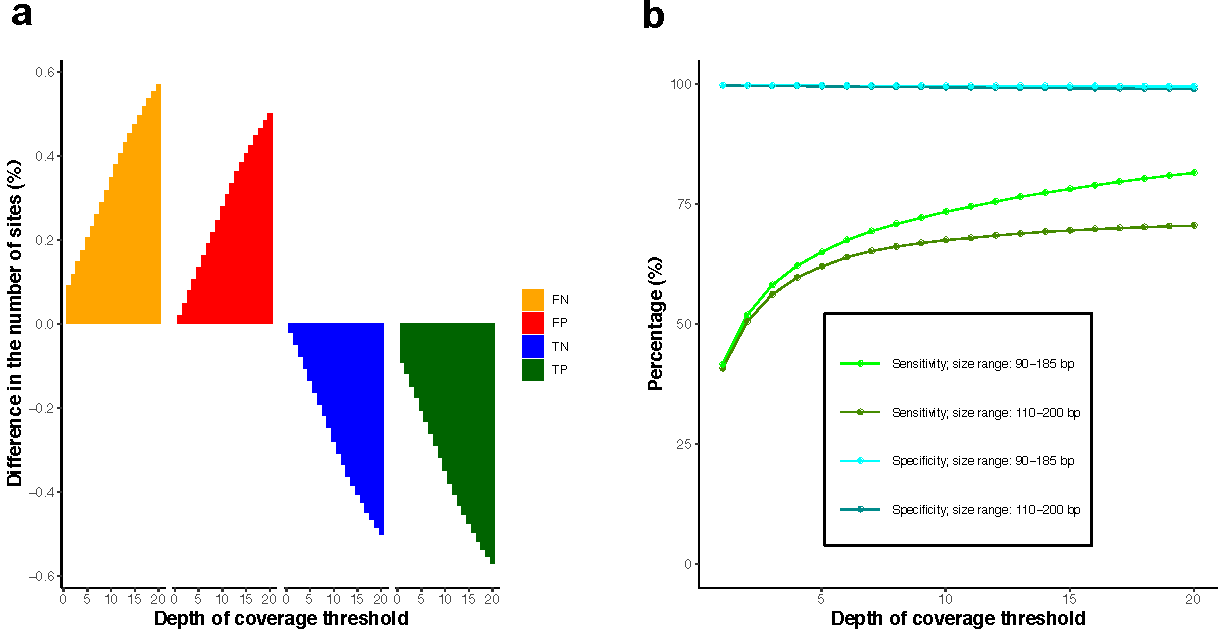
\includegraphics[width=1.0\textwidth]{SC4_Fig6}
	\vspace*{2mm}
	\caption[Effect of experimental errors during size selection in cuRRBS predictions]{Effect of experimental errors during size selection in cuRRBS predictions. \textbf{a.} Barplots showing the difference in the number of true positives (TP, in green), true negatives (TN, in blue), false positives (FP, in red) and false negatives (FN, in yellow) derived from cuRRBS theoretical predictions for the XmaI-RRBS data \cite{Tanas2017} using two different size ranges: 110-200 bp (aimed size range) and 90-185 bp (real size range). The difference observed between the two size ranges (aimed - real) is expressed as the percentage of the total number of sites considered (i.e. all CGI- CpGs). The number of sites in each category is calculated for different thresholds in the depth of coverage (number of reads covering a CpG site as reported by Bismark). cuRRBS was run for XmaI with all the default parameters (with a \textit{read length} of 200 bp). Legend is displayed on the right hand side. \textbf{b.} Plot showing values of cuRRBS sensitivity and specificity as a function of the depth of coverage threshold employed to filter the experimental data \cite{Tanas2017}. The two size ranges considered in a. (aimed: 110-200 bp; real: 90-185 bp) are used for the calculations. Legend is displayed below the plot curves.}
	\label{fig:sc4_fig6}
\end{figure}

\begin{figure}[htbp!] 
	\centering    
	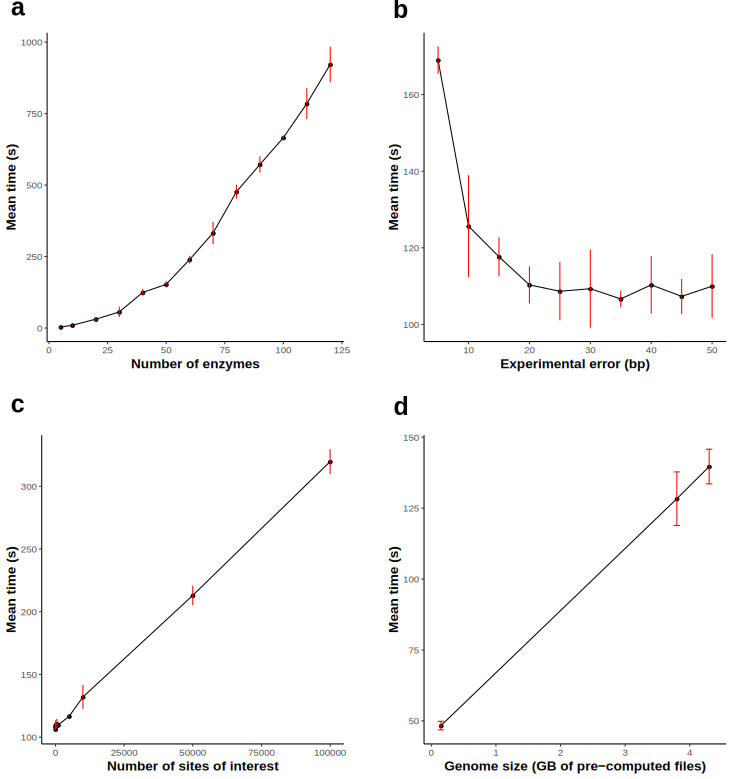
\includegraphics[width=0.8\textwidth]{SC4_Fig7}
	\vspace*{1mm}
	\caption[cuRRBS computational efficiency]{cuRRBS computational efficiency. \textbf{a.} Plot showing the dependency between the number of enzymes checked and the computational (real) time required by the software (mean between 3 independent runs). cuRRBS was run for the Horvath epigenetic clock system \cite{Horvath2013} with a \textit{read length} of 75 bp, a \textit{Score threshold} of $25\%$ and an \textit{experimental error} of 10 bp. A laptop with an Intel® Core$^{TM}$ i7-6600U CPU was used, which allowed cuRRBS to employ 4 parallel threads. The red error bars display the mean ± \acrshort{SD} for the 3 independent runs. \textbf{b.} Plot showing the dependency between the \textit{experimental error} (which determines how many size ranges are sampled) and the computational (real) time required by the software (mean between 3 independent runs). cuRRBS was run for the Horvath epigenetic clock system \cite{Horvath2013} with a \textit{read length} of 75 bp, a \textit{Score threshold} of $25\%$ and a list with 40 enzymes. A laptop with an Intel® Core$^{TM}$ i7-6600U CPU was used, which allowed cuRRBS to employ 4 parallel threads. The red error bars display the mean ± SD for the 3 independent runs. \textbf{c.} Plot showing the dependency between the number of sites of interest and the computational (real) time required by the software (mean between 3 independent runs). cuRRBS was run with a \textit{read length} of 75 bp, a \textit{Score threshold} of $25\%$, an \textit{experimental error} of 10 bp and a list with 40 enzymes. A laptop with an Intel® Core$^{TM}$ i7-6600U CPU was used, which allowed cuRRBS to employ 4 parallel threads. The red error bars display the mean ± SD for the 3 independent runs. \textbf{d.} Plot showing the dependency between genome size (measured as the size in GB of all the pre-computed files) and the computational (real) time required by the software (mean between 3 independent runs). cuRRBS was run with a \textit{read length} of 75 bp, a \textit{Score threshold} of $25\%$, an experimental error of 10 bp and a list with 40 enzymes. A laptop with an Intel® Core$^{TM}$ i7-6600U CPU was used, which allowed cuRRBS to employ 4 parallel threads. The red error bars display the mean ± SD for the 3 independent runs.}
	\label{fig:sc4_fig7}
\end{figure}


